\documentclass[twoside]{book}

% Packages required by doxygen
\usepackage{fixltx2e}
\usepackage{calc}
\usepackage{doxygen}
\usepackage[export]{adjustbox} % also loads graphicx
\usepackage{graphicx}
\usepackage[utf8]{inputenc}
\usepackage{makeidx}
\usepackage{multicol}
\usepackage{multirow}
\PassOptionsToPackage{warn}{textcomp}
\usepackage{textcomp}
\usepackage[nointegrals]{wasysym}
\usepackage[table]{xcolor}

% Font selection
\usepackage[T1]{fontenc}
\usepackage[scaled=.90]{helvet}
\usepackage{courier}
\usepackage{amssymb}
\usepackage{sectsty}
\renewcommand{\familydefault}{\sfdefault}
\allsectionsfont{%
  \fontseries{bc}\selectfont%
  \color{darkgray}%
}
\renewcommand{\DoxyLabelFont}{%
  \fontseries{bc}\selectfont%
  \color{darkgray}%
}
\newcommand{\+}{\discretionary{\mbox{\scriptsize$\hookleftarrow$}}{}{}}

% Page & text layout
\usepackage{geometry}
\geometry{%
  a4paper,%
  top=2.5cm,%
  bottom=2.5cm,%
  left=2.5cm,%
  right=2.5cm%
}
\tolerance=750
\hfuzz=15pt
\hbadness=750
\setlength{\emergencystretch}{15pt}
\setlength{\parindent}{0cm}
\setlength{\parskip}{0.2cm}
\makeatletter
\renewcommand{\paragraph}{%
  \@startsection{paragraph}{4}{0ex}{-1.0ex}{1.0ex}{%
    \normalfont\normalsize\bfseries\SS@parafont%
  }%
}
\renewcommand{\subparagraph}{%
  \@startsection{subparagraph}{5}{0ex}{-1.0ex}{1.0ex}{%
    \normalfont\normalsize\bfseries\SS@subparafont%
  }%
}
\makeatother

% Headers & footers
\usepackage{fancyhdr}
\pagestyle{fancyplain}
\fancyhead[LE]{\fancyplain{}{\bfseries\thepage}}
\fancyhead[CE]{\fancyplain{}{}}
\fancyhead[RE]{\fancyplain{}{\bfseries\leftmark}}
\fancyhead[LO]{\fancyplain{}{\bfseries\rightmark}}
\fancyhead[CO]{\fancyplain{}{}}
\fancyhead[RO]{\fancyplain{}{\bfseries\thepage}}
\fancyfoot[LE]{\fancyplain{}{}}
\fancyfoot[CE]{\fancyplain{}{}}
\fancyfoot[RE]{\fancyplain{}{\bfseries\scriptsize Generated on Wed Sep 30 2015 12\+:00\+:21 for My Project by Doxygen }}
\fancyfoot[LO]{\fancyplain{}{\bfseries\scriptsize Generated on Wed Sep 30 2015 12\+:00\+:21 for My Project by Doxygen }}
\fancyfoot[CO]{\fancyplain{}{}}
\fancyfoot[RO]{\fancyplain{}{}}
\renewcommand{\footrulewidth}{0.4pt}
\renewcommand{\chaptermark}[1]{%
  \markboth{#1}{}%
}
\renewcommand{\sectionmark}[1]{%
  \markright{\thesection\ #1}%
}

% Indices & bibliography
\usepackage{natbib}
\usepackage[titles]{tocloft}
\setcounter{tocdepth}{3}
\setcounter{secnumdepth}{5}
\makeindex

% Hyperlinks (required, but should be loaded last)
\usepackage{ifpdf}
\ifpdf
  \usepackage[pdftex,pagebackref=true]{hyperref}
\else
  \usepackage[ps2pdf,pagebackref=true]{hyperref}
\fi
\hypersetup{%
  colorlinks=true,%
  linkcolor=blue,%
  citecolor=blue,%
  unicode%
}

% Custom commands
\newcommand{\clearemptydoublepage}{%
  \newpage{\pagestyle{empty}\cleardoublepage}%
}


%===== C O N T E N T S =====

\begin{document}

% Titlepage & ToC
\hypersetup{pageanchor=false,
             bookmarks=true,
             bookmarksnumbered=true,
             pdfencoding=unicode
            }
\pagenumbering{roman}
\begin{titlepage}
\vspace*{7cm}
\begin{center}%
{\Large My Project }\\
\vspace*{1cm}
{\large Generated by Doxygen 1.8.9.1}\\
\vspace*{0.5cm}
{\small Wed Sep 30 2015 12:00:21}\\
\end{center}
\end{titlepage}
\clearemptydoublepage
\tableofcontents
\clearemptydoublepage
\pagenumbering{arabic}
\hypersetup{pageanchor=true}

%--- Begin generated contents ---
\chapter{Namespace Index}
\section{Packages}
Here are the packages with brief descriptions (if available)\+:\begin{DoxyCompactList}
\item\contentsline{section}{\hyperlink{namespace_contour___e_t}{Contour\+\_\+\+E\+T} }{\pageref{namespace_contour___e_t}}{}
\item\contentsline{section}{\hyperlink{namespacedocutil__text}{docutil\+\_\+text} }{\pageref{namespacedocutil__text}}{}
\item\contentsline{section}{\hyperlink{namespace_d_r___e_c}{D\+R\+\_\+\+E\+C} }{\pageref{namespace_d_r___e_c}}{}
\item\contentsline{section}{\hyperlink{namespaceet__util}{et\+\_\+util} }{\pageref{namespaceet__util}}{}
\item\contentsline{section}{\hyperlink{namespace_flag_analysis}{Flag\+Analysis} }{\pageref{namespace_flag_analysis}}{}
\item\contentsline{section}{\hyperlink{namespacegap_tests}{gap\+Tests} }{\pageref{namespacegap_tests}}{}
\item\contentsline{section}{\hyperlink{namespaceheatmap__slopes}{heatmap\+\_\+slopes} }{\pageref{namespaceheatmap__slopes}}{}
\item\contentsline{section}{\hyperlink{namespaceheatmap__subplots}{heatmap\+\_\+subplots} }{\pageref{namespaceheatmap__subplots}}{}
\item\contentsline{section}{\hyperlink{namespaceoptimum__growing__season}{optimum\+\_\+growing\+\_\+season} }{\pageref{namespaceoptimum__growing__season}}{}
\item\contentsline{section}{\hyperlink{namespace_preprocess}{Preprocess} \\*E\+T }{\pageref{namespace_preprocess}}{}
\item\contentsline{section}{\hyperlink{namespace_preprocess_01_d_r}{Preprocess D\+R} }{\pageref{namespace_preprocess_01_d_r}}{}
\item\contentsline{section}{\hyperlink{namespace_preprocess_01_e_t}{Preprocess E\+T} }{\pageref{namespace_preprocess_01_e_t}}{}
\item\contentsline{section}{\hyperlink{namespaces__post__process}{s\+\_\+post\+\_\+process} }{\pageref{namespaces__post__process}}{}
\end{DoxyCompactList}

\chapter{File Index}
\section{File List}
Here is a list of all files with brief descriptions\+:\begin{DoxyCompactList}
\item\contentsline{section}{\hyperlink{_contour___e_t_8py}{Contour\+\_\+\+E\+T.\+py} }{\pageref{_contour___e_t_8py}}{}
\item\contentsline{section}{\hyperlink{docutil__text_8py}{docutil\+\_\+text.\+py} }{\pageref{docutil__text_8py}}{}
\item\contentsline{section}{\hyperlink{_d_r___e_c_8py}{D\+R\+\_\+\+E\+C.\+py} }{\pageref{_d_r___e_c_8py}}{}
\item\contentsline{section}{\hyperlink{et__util_8py}{et\+\_\+util.\+py} }{\pageref{et__util_8py}}{}
\item\contentsline{section}{\hyperlink{_flag_analysis_8py}{Flag\+Analysis.\+py} }{\pageref{_flag_analysis_8py}}{}
\item\contentsline{section}{\hyperlink{gap_tests_8py}{gap\+Tests.\+py} }{\pageref{gap_tests_8py}}{}
\item\contentsline{section}{\hyperlink{heatmap__slopes_8py}{heatmap\+\_\+slopes.\+py} }{\pageref{heatmap__slopes_8py}}{}
\item\contentsline{section}{\hyperlink{heatmap__subplots_8py}{heatmap\+\_\+subplots.\+py} }{\pageref{heatmap__subplots_8py}}{}
\item\contentsline{section}{\hyperlink{optimum__growing__season_8py}{optimum\+\_\+growing\+\_\+season.\+py} }{\pageref{optimum__growing__season_8py}}{}
\item\contentsline{section}{\hyperlink{_preprocess_01_d_r_8py}{Preprocess D\+R.\+py} }{\pageref{_preprocess_01_d_r_8py}}{}
\item\contentsline{section}{\hyperlink{_preprocess_01_e_t_8py}{Preprocess E\+T.\+py} }{\pageref{_preprocess_01_e_t_8py}}{}
\item\contentsline{section}{\hyperlink{s__post__process_8py}{s\+\_\+post\+\_\+process.\+py} }{\pageref{s__post__process_8py}}{}
\end{DoxyCompactList}

\chapter{Namespace Documentation}
\hypertarget{namespace_contour___e_t}{}\section{Contour\+\_\+\+E\+T Namespace Reference}
\label{namespace_contour___e_t}\index{Contour\+\_\+\+E\+T@{Contour\+\_\+\+E\+T}}
\subsection*{Functions}
\begin{DoxyCompactItemize}
\item 
def \hyperlink{namespace_contour___e_t_a4fecac488658fd1b99977ef8e39d5b5b}{get\+\_\+colors} (num\+\_\+colors)
\item 
def \hyperlink{namespace_contour___e_t_aedcf6d62d60dabb84683309eaa07b36c}{get\+\_\+df\+\_\+from\+\_\+file} (path\+\_\+name)
\item 
def \hyperlink{namespace_contour___e_t_aa24aa07cccaaf85a6757f39c28f31f8c}{refactor\+\_\+time} (\hyperlink{namespace_contour___e_t_ada636549e35711b9f1d5830a945e5472}{df})
\item 
def \hyperlink{namespace_contour___e_t_ae9bd39a079647783c05dbe6639ef91a5}{save\+\_\+to\+\_\+csv} (\hyperlink{namespace_contour___e_t_ada636549e35711b9f1d5830a945e5472}{df}, path\+\_\+name)
\item 
def \hyperlink{namespace_contour___e_t_a4c29753b8fe8e656b9b45e445b43f691}{relabel\+\_\+axis} (axis, plt)
\item 
def \hyperlink{namespace_contour___e_t_a90148b8c5b469f8ba98e2d231b2fb45b}{make\+\_\+contour} (\hyperlink{namespace_contour___e_t_ada636549e35711b9f1d5830a945e5472}{df}, \hyperlink{namespace_contour___e_t_afe10e2d562af1d0f4be9cc7b17a68e49}{df\+\_\+piv})
\end{DoxyCompactItemize}
\subsection*{Variables}
\begin{DoxyCompactItemize}
\item 
string \hyperlink{namespace_contour___e_t_a7af933d5513c2211e9381ded4aa968f8}{\+\_\+\+\_\+author\+\_\+\+\_\+} = \textquotesingle{}mturtora\textquotesingle{}
\item 
string \hyperlink{namespace_contour___e_t_af326a717be24fa633d2faf0eac687552}{path} = \textquotesingle{}..\textbackslash{}\textbackslash{}..\textbackslash{}\textbackslash{}Starkey\textbackslash{}\textbackslash{}process\textbackslash{}\textbackslash{}201505\textbackslash{}\textbackslash{}\textquotesingle{}
\item 
string \hyperlink{namespace_contour___e_t_a1d101debf10ad92d73509b40746b119c}{pivot\+\_\+column\+\_\+name} = \textquotesingle{}E\+T\textquotesingle{}
\item 
tuple \hyperlink{namespace_contour___e_t_ada636549e35711b9f1d5830a945e5472}{df} = \hyperlink{namespace_contour___e_t_aedcf6d62d60dabb84683309eaa07b36c}{get\+\_\+df\+\_\+from\+\_\+file}(\hyperlink{namespace_contour___e_t_af326a717be24fa633d2faf0eac687552}{path} + \textquotesingle{}Flag\+Analysis.\+csv\textquotesingle{})
\item 
tuple \hyperlink{namespace_contour___e_t_afe10e2d562af1d0f4be9cc7b17a68e49}{df\+\_\+piv} = df.\+pivot(index=\textquotesingle{}dates\textquotesingle{}, columns=\textquotesingle{}times\textquotesingle{}, values=\hyperlink{namespace_contour___e_t_a1d101debf10ad92d73509b40746b119c}{pivot\+\_\+column\+\_\+name})
\end{DoxyCompactItemize}


\subsection{Function Documentation}
\hypertarget{namespace_contour___e_t_a4fecac488658fd1b99977ef8e39d5b5b}{}\index{Contour\+\_\+\+E\+T@{Contour\+\_\+\+E\+T}!get\+\_\+colors@{get\+\_\+colors}}
\index{get\+\_\+colors@{get\+\_\+colors}!Contour\+\_\+\+E\+T@{Contour\+\_\+\+E\+T}}
\subsubsection[{get\+\_\+colors}]{\setlength{\rightskip}{0pt plus 5cm}def Contour\+\_\+\+E\+T.\+get\+\_\+colors (
\begin{DoxyParamCaption}
\item[{}]{num\+\_\+colors}
\end{DoxyParamCaption}
)}\label{namespace_contour___e_t_a4fecac488658fd1b99977ef8e39d5b5b}


Definition at line 3 of file Contour\+\_\+\+E\+T.\+py.

\hypertarget{namespace_contour___e_t_aedcf6d62d60dabb84683309eaa07b36c}{}\index{Contour\+\_\+\+E\+T@{Contour\+\_\+\+E\+T}!get\+\_\+df\+\_\+from\+\_\+file@{get\+\_\+df\+\_\+from\+\_\+file}}
\index{get\+\_\+df\+\_\+from\+\_\+file@{get\+\_\+df\+\_\+from\+\_\+file}!Contour\+\_\+\+E\+T@{Contour\+\_\+\+E\+T}}
\subsubsection[{get\+\_\+df\+\_\+from\+\_\+file}]{\setlength{\rightskip}{0pt plus 5cm}def Contour\+\_\+\+E\+T.\+get\+\_\+df\+\_\+from\+\_\+file (
\begin{DoxyParamCaption}
\item[{}]{path\+\_\+name}
\end{DoxyParamCaption}
)}\label{namespace_contour___e_t_aedcf6d62d60dabb84683309eaa07b36c}


Definition at line 15 of file Contour\+\_\+\+E\+T.\+py.

\hypertarget{namespace_contour___e_t_a90148b8c5b469f8ba98e2d231b2fb45b}{}\index{Contour\+\_\+\+E\+T@{Contour\+\_\+\+E\+T}!make\+\_\+contour@{make\+\_\+contour}}
\index{make\+\_\+contour@{make\+\_\+contour}!Contour\+\_\+\+E\+T@{Contour\+\_\+\+E\+T}}
\subsubsection[{make\+\_\+contour}]{\setlength{\rightskip}{0pt plus 5cm}def Contour\+\_\+\+E\+T.\+make\+\_\+contour (
\begin{DoxyParamCaption}
\item[{}]{df, }
\item[{}]{df\+\_\+piv}
\end{DoxyParamCaption}
)}\label{namespace_contour___e_t_a90148b8c5b469f8ba98e2d231b2fb45b}
\begin{DoxyVerb}Contour plot of date and time data.  Could improve by combining df and df_piv

:param df: dataframe with date and time vectors
:param df_piv: dataframe with array data
:return: nothing, plots to screen
\end{DoxyVerb}
 

Definition at line 59 of file Contour\+\_\+\+E\+T.\+py.



Here is the call graph for this function\+:\nopagebreak
\begin{figure}[H]
\begin{center}
\leavevmode
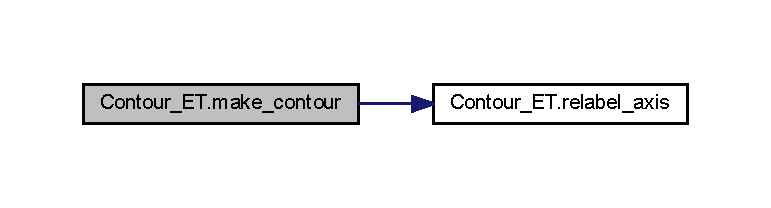
\includegraphics[width=350pt]{namespace_contour___e_t_a90148b8c5b469f8ba98e2d231b2fb45b_cgraph}
\end{center}
\end{figure}


\hypertarget{namespace_contour___e_t_aa24aa07cccaaf85a6757f39c28f31f8c}{}\index{Contour\+\_\+\+E\+T@{Contour\+\_\+\+E\+T}!refactor\+\_\+time@{refactor\+\_\+time}}
\index{refactor\+\_\+time@{refactor\+\_\+time}!Contour\+\_\+\+E\+T@{Contour\+\_\+\+E\+T}}
\subsubsection[{refactor\+\_\+time}]{\setlength{\rightskip}{0pt plus 5cm}def Contour\+\_\+\+E\+T.\+refactor\+\_\+time (
\begin{DoxyParamCaption}
\item[{}]{df}
\end{DoxyParamCaption}
)}\label{namespace_contour___e_t_aa24aa07cccaaf85a6757f39c28f31f8c}
\begin{DoxyVerb}Extracts day fraction and year

:param df:
:return:
\end{DoxyVerb}
 

Definition at line 19 of file Contour\+\_\+\+E\+T.\+py.

\hypertarget{namespace_contour___e_t_a4c29753b8fe8e656b9b45e445b43f691}{}\index{Contour\+\_\+\+E\+T@{Contour\+\_\+\+E\+T}!relabel\+\_\+axis@{relabel\+\_\+axis}}
\index{relabel\+\_\+axis@{relabel\+\_\+axis}!Contour\+\_\+\+E\+T@{Contour\+\_\+\+E\+T}}
\subsubsection[{relabel\+\_\+axis}]{\setlength{\rightskip}{0pt plus 5cm}def Contour\+\_\+\+E\+T.\+relabel\+\_\+axis (
\begin{DoxyParamCaption}
\item[{}]{axis, }
\item[{}]{plt}
\end{DoxyParamCaption}
)}\label{namespace_contour___e_t_a4c29753b8fe8e656b9b45e445b43f691}
\begin{DoxyVerb}Don't like axis format for (hours, years) so redo

:param axis: string, 'x' or 'y'
:param plt: imshow plot object
:return: x or y ticks vectors of locs and labels
\end{DoxyVerb}
 

Definition at line 37 of file Contour\+\_\+\+E\+T.\+py.



Here is the caller graph for this function\+:\nopagebreak
\begin{figure}[H]
\begin{center}
\leavevmode
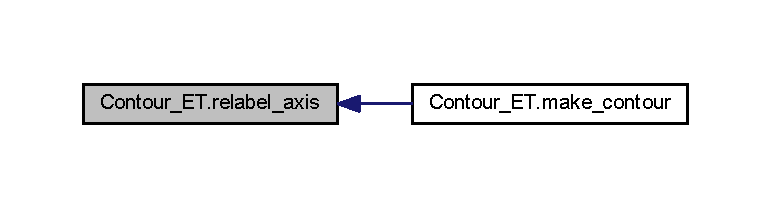
\includegraphics[width=350pt]{namespace_contour___e_t_a4c29753b8fe8e656b9b45e445b43f691_icgraph}
\end{center}
\end{figure}


\hypertarget{namespace_contour___e_t_ae9bd39a079647783c05dbe6639ef91a5}{}\index{Contour\+\_\+\+E\+T@{Contour\+\_\+\+E\+T}!save\+\_\+to\+\_\+csv@{save\+\_\+to\+\_\+csv}}
\index{save\+\_\+to\+\_\+csv@{save\+\_\+to\+\_\+csv}!Contour\+\_\+\+E\+T@{Contour\+\_\+\+E\+T}}
\subsubsection[{save\+\_\+to\+\_\+csv}]{\setlength{\rightskip}{0pt plus 5cm}def Contour\+\_\+\+E\+T.\+save\+\_\+to\+\_\+csv (
\begin{DoxyParamCaption}
\item[{}]{df, }
\item[{}]{path\+\_\+name}
\end{DoxyParamCaption}
)}\label{namespace_contour___e_t_ae9bd39a079647783c05dbe6639ef91a5}


Definition at line 33 of file Contour\+\_\+\+E\+T.\+py.



\subsection{Variable Documentation}
\hypertarget{namespace_contour___e_t_a7af933d5513c2211e9381ded4aa968f8}{}\index{Contour\+\_\+\+E\+T@{Contour\+\_\+\+E\+T}!\+\_\+\+\_\+author\+\_\+\+\_\+@{\+\_\+\+\_\+author\+\_\+\+\_\+}}
\index{\+\_\+\+\_\+author\+\_\+\+\_\+@{\+\_\+\+\_\+author\+\_\+\+\_\+}!Contour\+\_\+\+E\+T@{Contour\+\_\+\+E\+T}}
\subsubsection[{\+\_\+\+\_\+author\+\_\+\+\_\+}]{\setlength{\rightskip}{0pt plus 5cm}string Contour\+\_\+\+E\+T.\+\_\+\+\_\+author\+\_\+\+\_\+ = \textquotesingle{}mturtora\textquotesingle{}}\label{namespace_contour___e_t_a7af933d5513c2211e9381ded4aa968f8}


Definition at line 110 of file Contour\+\_\+\+E\+T.\+py.

\hypertarget{namespace_contour___e_t_ada636549e35711b9f1d5830a945e5472}{}\index{Contour\+\_\+\+E\+T@{Contour\+\_\+\+E\+T}!df@{df}}
\index{df@{df}!Contour\+\_\+\+E\+T@{Contour\+\_\+\+E\+T}}
\subsubsection[{df}]{\setlength{\rightskip}{0pt plus 5cm}tuple Contour\+\_\+\+E\+T.\+df = {\bf get\+\_\+df\+\_\+from\+\_\+file}({\bf path} + \textquotesingle{}Flag\+Analysis.\+csv\textquotesingle{})}\label{namespace_contour___e_t_ada636549e35711b9f1d5830a945e5472}


Definition at line 117 of file Contour\+\_\+\+E\+T.\+py.

\hypertarget{namespace_contour___e_t_afe10e2d562af1d0f4be9cc7b17a68e49}{}\index{Contour\+\_\+\+E\+T@{Contour\+\_\+\+E\+T}!df\+\_\+piv@{df\+\_\+piv}}
\index{df\+\_\+piv@{df\+\_\+piv}!Contour\+\_\+\+E\+T@{Contour\+\_\+\+E\+T}}
\subsubsection[{df\+\_\+piv}]{\setlength{\rightskip}{0pt plus 5cm}tuple Contour\+\_\+\+E\+T.\+df\+\_\+piv = df.\+pivot(index=\textquotesingle{}dates\textquotesingle{}, columns=\textquotesingle{}times\textquotesingle{}, values={\bf pivot\+\_\+column\+\_\+name})}\label{namespace_contour___e_t_afe10e2d562af1d0f4be9cc7b17a68e49}


Definition at line 125 of file Contour\+\_\+\+E\+T.\+py.

\hypertarget{namespace_contour___e_t_af326a717be24fa633d2faf0eac687552}{}\index{Contour\+\_\+\+E\+T@{Contour\+\_\+\+E\+T}!path@{path}}
\index{path@{path}!Contour\+\_\+\+E\+T@{Contour\+\_\+\+E\+T}}
\subsubsection[{path}]{\setlength{\rightskip}{0pt plus 5cm}string Contour\+\_\+\+E\+T.\+path = \textquotesingle{}..\textbackslash{}\textbackslash{}..\textbackslash{}\textbackslash{}Starkey\textbackslash{}\textbackslash{}process\textbackslash{}\textbackslash{}201505\textbackslash{}\textbackslash{}\textquotesingle{}}\label{namespace_contour___e_t_af326a717be24fa633d2faf0eac687552}


Definition at line 115 of file Contour\+\_\+\+E\+T.\+py.

\hypertarget{namespace_contour___e_t_a1d101debf10ad92d73509b40746b119c}{}\index{Contour\+\_\+\+E\+T@{Contour\+\_\+\+E\+T}!pivot\+\_\+column\+\_\+name@{pivot\+\_\+column\+\_\+name}}
\index{pivot\+\_\+column\+\_\+name@{pivot\+\_\+column\+\_\+name}!Contour\+\_\+\+E\+T@{Contour\+\_\+\+E\+T}}
\subsubsection[{pivot\+\_\+column\+\_\+name}]{\setlength{\rightskip}{0pt plus 5cm}string Contour\+\_\+\+E\+T.\+pivot\+\_\+column\+\_\+name = \textquotesingle{}E\+T\textquotesingle{}}\label{namespace_contour___e_t_a1d101debf10ad92d73509b40746b119c}


Definition at line 116 of file Contour\+\_\+\+E\+T.\+py.


\hypertarget{namespacedocutil__text}{}\section{docutil\+\_\+text Namespace Reference}
\label{namespacedocutil__text}\index{docutil\+\_\+text@{docutil\+\_\+text}}
\subsection*{Variables}
\begin{DoxyCompactItemize}
\item 
string \hyperlink{namespacedocutil__text_a29c40c7a34ccbc2912a2de0125ac51fa}{\+\_\+\+\_\+author\+\_\+\+\_\+} = \textquotesingle{}mturtora\textquotesingle{}
\end{DoxyCompactItemize}


\subsection{Variable Documentation}
\hypertarget{namespacedocutil__text_a29c40c7a34ccbc2912a2de0125ac51fa}{}\index{docutil\+\_\+text@{docutil\+\_\+text}!\+\_\+\+\_\+author\+\_\+\+\_\+@{\+\_\+\+\_\+author\+\_\+\+\_\+}}
\index{\+\_\+\+\_\+author\+\_\+\+\_\+@{\+\_\+\+\_\+author\+\_\+\+\_\+}!docutil\+\_\+text@{docutil\+\_\+text}}
\subsubsection[{\+\_\+\+\_\+author\+\_\+\+\_\+}]{\setlength{\rightskip}{0pt plus 5cm}string docutil\+\_\+text.\+\_\+\+\_\+author\+\_\+\+\_\+ = \textquotesingle{}mturtora\textquotesingle{}}\label{namespacedocutil__text_a29c40c7a34ccbc2912a2de0125ac51fa}


Definition at line 1 of file docutil\+\_\+text.\+py.


\hypertarget{namespace_d_r___e_c}{}\section{D\+R\+\_\+\+E\+C Namespace Reference}
\label{namespace_d_r___e_c}\index{D\+R\+\_\+\+E\+C@{D\+R\+\_\+\+E\+C}}
\subsection*{Variables}
\begin{DoxyCompactItemize}
\item 
string \hyperlink{namespace_d_r___e_c_a9a613c3082ebba655a69e69185821879}{f} = \textquotesingle{}D\+R\+\_\+\+E\+C.\+dat\textquotesingle{}
\item 
tuple \hyperlink{namespace_d_r___e_c_a849f81e16400fa6ef7c269c894aa32e2}{df} = et.\+get\+\_\+df(\hyperlink{namespace_d_r___e_c_a9a613c3082ebba655a69e69185821879}{f}, \textquotesingle{}ec\textquotesingle{}, \textquotesingle{}csv\textquotesingle{}, \textquotesingle{}d\textquotesingle{})
\end{DoxyCompactItemize}


\subsection{Variable Documentation}
\hypertarget{namespace_d_r___e_c_a849f81e16400fa6ef7c269c894aa32e2}{}\index{D\+R\+\_\+\+E\+C@{D\+R\+\_\+\+E\+C}!df@{df}}
\index{df@{df}!D\+R\+\_\+\+E\+C@{D\+R\+\_\+\+E\+C}}
\subsubsection[{df}]{\setlength{\rightskip}{0pt plus 5cm}tuple D\+R\+\_\+\+E\+C.\+df = et.\+get\+\_\+df({\bf f}, \textquotesingle{}ec\textquotesingle{}, \textquotesingle{}csv\textquotesingle{}, \textquotesingle{}d\textquotesingle{})}\label{namespace_d_r___e_c_a849f81e16400fa6ef7c269c894aa32e2}


Definition at line 10 of file D\+R\+\_\+\+E\+C.\+py.

\hypertarget{namespace_d_r___e_c_a9a613c3082ebba655a69e69185821879}{}\index{D\+R\+\_\+\+E\+C@{D\+R\+\_\+\+E\+C}!f@{f}}
\index{f@{f}!D\+R\+\_\+\+E\+C@{D\+R\+\_\+\+E\+C}}
\subsubsection[{f}]{\setlength{\rightskip}{0pt plus 5cm}string D\+R\+\_\+\+E\+C.\+f = \textquotesingle{}D\+R\+\_\+\+E\+C.\+dat\textquotesingle{}}\label{namespace_d_r___e_c_a9a613c3082ebba655a69e69185821879}


Definition at line 9 of file D\+R\+\_\+\+E\+C.\+py.


\hypertarget{namespaceet__util}{}\section{et\+\_\+util Namespace Reference}
\label{namespaceet__util}\index{et\+\_\+util@{et\+\_\+util}}
\subsection*{Functions}
\begin{DoxyCompactItemize}
\item 
def \hyperlink{namespaceet__util_a164b6705ccf94cb947d6bd11c7c19021}{startup} (path\+\_\+in, path\+\_\+out, path\+\_\+temp, station, station\+\_\+prefix, analysis\+\_\+start, release\+\_\+start, release\+\_\+end, rebuild, combined\+\_\+echo, echo\+\_\+get)
\item 
def \hyperlink{namespaceet__util_ad79d083c0b67b0c0aa1c3f9f247bf856}{confirm\+\_\+rebuild} (info\+\_\+message, prompt\+\_\+message, sys\+\_\+message)
\item 
def \hyperlink{namespaceet__util_a3c3ae2439b3b5337237d456cb4366028}{get\+\_\+file\+\_\+times} (config)
\item 
def \hyperlink{namespaceet__util_aa4a0538c05ece93097940be5a2ef4204}{write\+\_\+file\+\_\+times} (config, release\+\_\+start, release\+\_\+end)
\item 
def \hyperlink{namespaceet__util_a7d463c3690915efb78c87700565efc77}{clean\+\_\+file} (path\+\_\+in, path\+\_\+temp, fname)
\item 
def \hyperlink{namespaceet__util_ad14756ce8dfea7ab6da605eb2a34af45}{inventory} (path\+\_\+in, path\+\_\+out, path\+\_\+temp, station, station\+\_\+prefix, analysis\+\_\+start, combined\+\_\+echo, echo\+\_\+get)
\item 
def \hyperlink{namespaceet__util_a241e2fa8182c03412e519a4c6431d29b}{met\+\_\+filter} (df\+\_\+met, station)
\item 
def \hyperlink{namespaceet__util_ac2422e9d685033121b1c6739352cf345}{convert\+\_\+precip} (df)
\item 
def \hyperlink{namespaceet__util_a51bdba14dfab7dd5e7884cec009abde7}{apply\+\_\+edits} (path\+\_\+out, df)
\item 
def \hyperlink{namespaceet__util_a3331dc365022196889cfcd3fa3cca3b2}{join\+\_\+and\+\_\+delete} (df, path\+\_\+out, fname, delete\+\_\+list)
\item 
def \hyperlink{namespaceet__util_adf3e6bef75b663226a9c118684f91689}{read\+\_\+files} (path\+\_\+out)
\item 
def \hyperlink{namespaceet__util_a41b39b3c70ba9961221c284cc738122e}{write\+\_\+raw} (path\+\_\+out, df\+\_\+met, df\+\_\+rad, df\+\_\+ec, df\+\_\+ec\+\_\+all)
\item 
def \hyperlink{namespaceet__util_afe6d9320f59488fc7e462d7c501e828d}{concat\+\_\+df}
\item 
def \hyperlink{namespaceet__util_a8013dc0897f9430ae8f354ba094b9fbd}{get\+\_\+df} (fname, df\+\_\+type, out\+\_\+form, station, echo\+\_\+get)
\item 
def \hyperlink{namespaceet__util_a7535fb2ada235d852a05717bdd6d67a9}{read\+\_\+s\+\_\+ec}
\item 
def \hyperlink{namespaceet__util_a5cda9dc3d34bdd80d01b977e805f4b04}{read\+\_\+d\+\_\+ec}
\item 
def \hyperlink{namespaceet__util_a5cfb9371164d33036c4d3ec9f7a80e88}{read\+\_\+s\+\_\+met} (f)
\item 
def \hyperlink{namespaceet__util_aa20b5ae88dbfb272ae5e7f53f4678358}{read\+\_\+d\+\_\+met} (f)
\item 
def \hyperlink{namespaceet__util_a37255b034ed791b14cb66dc5df649a3f}{read\+\_\+s\+\_\+rad} (f)
\item 
def \hyperlink{namespaceet__util_a76d5a5c19f0e86b9ab70c0957827c260}{read\+\_\+d\+\_\+rad} (f)
\item 
def \hyperlink{namespaceet__util_add60caac6c3d8333a58794a411891f57}{doy\+\_\+parser} (year, doy, time)
\item 
def \hyperlink{namespaceet__util_a566ff749c2a2c113c58d24649251bd5b}{read\+\_\+\+C\+Rten\+X\+\_\+file} (path, fname, df\+\_\+type)
\item 
def \hyperlink{namespaceet__util_af15d3c41901948dbb10f0c796cb6ed5b}{read\+\_\+\+C\+Rthousand\+\_\+file} (f, fname)
\item 
def \hyperlink{namespaceet__util_a38dc0fbf4d56c116d7f8eb34a893abad}{select\+\_\+dates} (analysis\+\_\+start, release\+\_\+end, df\+\_\+met, df\+\_\+rad, df\+\_\+ec, df\+\_\+ec\+\_\+all)
\item 
def \hyperlink{namespaceet__util_a9d53464743ec890e7b0a9d367d09a6ad}{pad\+\_\+missing\+\_\+with\+\_\+nulls} (df\+\_\+pad, dtype)
\item 
def \hyperlink{namespaceet__util_a15b819dcfa7f04be44839a9887e62c41}{gap} (path, df0, dtype, make\+\_\+gap\+\_\+plots)
\item 
def \hyperlink{namespaceet__util_a86bdf627c5eafcab2d20a7d1ce75a1ed}{gap\+\_\+expand} (path\+\_\+out, column)
\item 
def \hyperlink{namespaceet__util_a90f4dcfab0e13429f6041ea3b2db13b4}{confirm\+\_\+plot} (info\+\_\+message, prompt\+\_\+message, sys\+\_\+message)
\item 
def \hyperlink{namespaceet__util_abf296bc00b589318395becdb4aa3f89d}{impute\+\_\+master} (path\+\_\+out, df)
\item 
def \hyperlink{namespaceet__util_ad991b40a8a99a7e5384f3bdfb1258af5}{impute\+\_\+strata} (path\+\_\+out, df, df\+\_\+month\+\_\+mn, column, mask)
\item 
def \hyperlink{namespaceet__util_ae6b0b0285532d32dd9d5d2b42c7f6043}{impute\+\_\+simple} (path\+\_\+out, df, dtype, print\+\_\+flag)
\item 
def \hyperlink{namespaceet__util_a28b3adad3d77922fccf7a1d77dd3adda}{s\+\_\+met\+\_\+calcs}
\item 
def \hyperlink{namespaceet__util_a45d34a2e8a980bed1bcf1c8d708399cc}{d\+\_\+met\+\_\+calcs}
\item 
def \hyperlink{namespaceet__util_a04161955cfa0207847c92471361582ae}{met\+\_\+fort} (path\+\_\+out, df\+\_\+out, station)
\item 
def \hyperlink{namespaceet__util_a4fd6a305cc0207763b1d2386f9eeac84}{ec\+\_\+fort} (df\+\_\+ec)
\item 
def \hyperlink{namespaceet__util_a8f87bce6dab1c42c9130fae0df312416}{to\+Year\+Fraction} (date)
\item 
def \hyperlink{namespaceet__util_a07507bce96a663ca49bd206aadc6272c}{df\+\_\+csv}
\item 
def \hyperlink{namespaceet__util_a15aa7ba554d08be6cbf6a674accfa16e}{echo\+\_\+description}
\item 
def \hyperlink{namespaceet__util_abbaa0589af07e21f8a1d98515aafef03}{df\+\_\+dat} (df\+\_\+v, fname)
\begin{DoxyCompactList}\small\item\em Orphan code functions. \end{DoxyCompactList}\item 
def \hyperlink{namespaceet__util_ad1b21b5159cbb574e683156c7870b06d}{missnaec} (df)
\end{DoxyCompactItemize}


\subsection{Detailed Description}
\begin{DoxyVerb}et_util.py
Functions for processing Tampa ET data.
\end{DoxyVerb}
 

\subsection{Function Documentation}
\hypertarget{namespaceet__util_a51bdba14dfab7dd5e7884cec009abde7}{}\index{et\+\_\+util@{et\+\_\+util}!apply\+\_\+edits@{apply\+\_\+edits}}
\index{apply\+\_\+edits@{apply\+\_\+edits}!et\+\_\+util@{et\+\_\+util}}
\subsubsection[{apply\+\_\+edits}]{\setlength{\rightskip}{0pt plus 5cm}def et\+\_\+util.\+apply\+\_\+edits (
\begin{DoxyParamCaption}
\item[{}]{path\+\_\+out, }
\item[{}]{df}
\end{DoxyParamCaption}
)}\label{namespaceet__util_a51bdba14dfab7dd5e7884cec009abde7}
\begin{DoxyVerb}Use external file of manually identified bad data to remove bad data.

:param path_out:
:param df:
:return:
\end{DoxyVerb}
 

Definition at line 462 of file et\+\_\+util.\+py.



Here is the call graph for this function\+:
\nopagebreak
\begin{figure}[H]
\begin{center}
\leavevmode
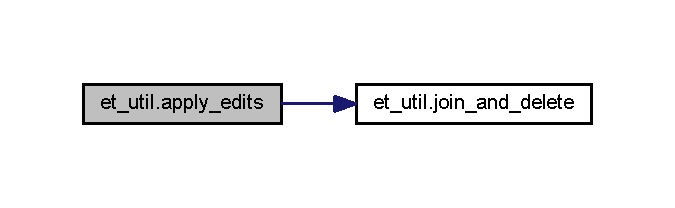
\includegraphics[width=324pt]{namespaceet__util_a51bdba14dfab7dd5e7884cec009abde7_cgraph}
\end{center}
\end{figure}




Here is the caller graph for this function\+:
\nopagebreak
\begin{figure}[H]
\begin{center}
\leavevmode
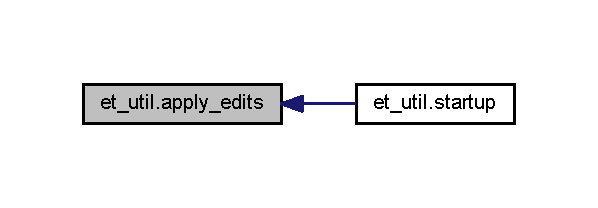
\includegraphics[width=287pt]{namespaceet__util_a51bdba14dfab7dd5e7884cec009abde7_icgraph}
\end{center}
\end{figure}


\hypertarget{namespaceet__util_a7d463c3690915efb78c87700565efc77}{}\index{et\+\_\+util@{et\+\_\+util}!clean\+\_\+file@{clean\+\_\+file}}
\index{clean\+\_\+file@{clean\+\_\+file}!et\+\_\+util@{et\+\_\+util}}
\subsubsection[{clean\+\_\+file}]{\setlength{\rightskip}{0pt plus 5cm}def et\+\_\+util.\+clean\+\_\+file (
\begin{DoxyParamCaption}
\item[{}]{path\+\_\+in, }
\item[{}]{path\+\_\+temp, }
\item[{}]{fname}
\end{DoxyParamCaption}
)}\label{namespaceet__util_a7d463c3690915efb78c87700565efc77}


Definition at line 208 of file et\+\_\+util.\+py.



Here is the call graph for this function\+:
\nopagebreak
\begin{figure}[H]
\begin{center}
\leavevmode
\includegraphics[width=350pt]{namespaceet__util_a7d463c3690915efb78c87700565efc77_cgraph}
\end{center}
\end{figure}




Here is the caller graph for this function\+:
\nopagebreak
\begin{figure}[H]
\begin{center}
\leavevmode
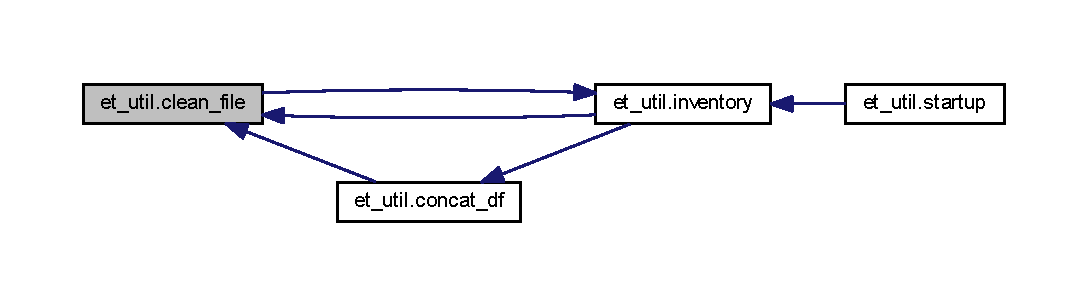
\includegraphics[width=350pt]{namespaceet__util_a7d463c3690915efb78c87700565efc77_icgraph}
\end{center}
\end{figure}


\hypertarget{namespaceet__util_afe6d9320f59488fc7e462d7c501e828d}{}\index{et\+\_\+util@{et\+\_\+util}!concat\+\_\+df@{concat\+\_\+df}}
\index{concat\+\_\+df@{concat\+\_\+df}!et\+\_\+util@{et\+\_\+util}}
\subsubsection[{concat\+\_\+df}]{\setlength{\rightskip}{0pt plus 5cm}def et\+\_\+util.\+concat\+\_\+df (
\begin{DoxyParamCaption}
\item[{}]{path\+\_\+in, }
\item[{}]{path\+\_\+temp, }
\item[{}]{flist, }
\item[{}]{df\+\_\+type, }
\item[{}]{station, }
\item[{}]{echo\+\_\+get = {\ttfamily False}, }
\item[{}]{out\+\_\+form = {\ttfamily \textquotesingle{}csv\textquotesingle{}}}
\end{DoxyParamCaption}
)}\label{namespaceet__util_afe6d9320f59488fc7e462d7c501e828d}
\begin{DoxyVerb}Concatenate given list of files using 'update.'

:rtype : object
:param path_in: Pathname to files
:param flist: List of files to combine
:param df_type: Data type
:param out_form: passed to get_df.  'csv' or not
:return: df_cat - DataFrame of combined data\end{DoxyVerb}
 

Definition at line 522 of file et\+\_\+util.\+py.



Here is the call graph for this function\+:\nopagebreak
\begin{figure}[H]
\begin{center}
\leavevmode
\includegraphics[width=350pt]{namespaceet__util_afe6d9320f59488fc7e462d7c501e828d_cgraph}
\end{center}
\end{figure}




Here is the caller graph for this function\+:
\nopagebreak
\begin{figure}[H]
\begin{center}
\leavevmode
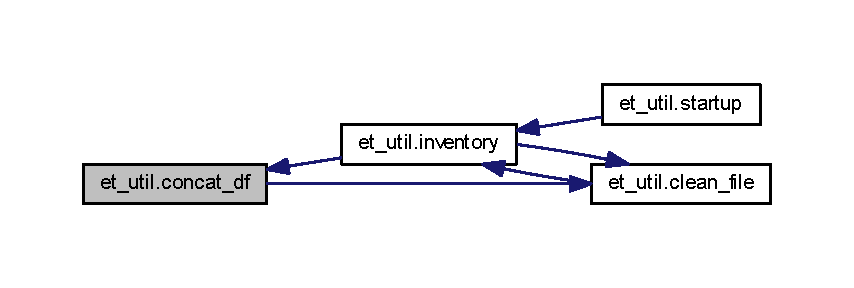
\includegraphics[width=350pt]{namespaceet__util_afe6d9320f59488fc7e462d7c501e828d_icgraph}
\end{center}
\end{figure}


\hypertarget{namespaceet__util_a90f4dcfab0e13429f6041ea3b2db13b4}{}\index{et\+\_\+util@{et\+\_\+util}!confirm\+\_\+plot@{confirm\+\_\+plot}}
\index{confirm\+\_\+plot@{confirm\+\_\+plot}!et\+\_\+util@{et\+\_\+util}}
\subsubsection[{confirm\+\_\+plot}]{\setlength{\rightskip}{0pt plus 5cm}def et\+\_\+util.\+confirm\+\_\+plot (
\begin{DoxyParamCaption}
\item[{}]{info\+\_\+message, }
\item[{}]{prompt\+\_\+message, }
\item[{}]{sys\+\_\+message}
\end{DoxyParamCaption}
)}\label{namespaceet__util_a90f4dcfab0e13429f6041ea3b2db13b4}


Definition at line 1098 of file et\+\_\+util.\+py.

\hypertarget{namespaceet__util_ad79d083c0b67b0c0aa1c3f9f247bf856}{}\index{et\+\_\+util@{et\+\_\+util}!confirm\+\_\+rebuild@{confirm\+\_\+rebuild}}
\index{confirm\+\_\+rebuild@{confirm\+\_\+rebuild}!et\+\_\+util@{et\+\_\+util}}
\subsubsection[{confirm\+\_\+rebuild}]{\setlength{\rightskip}{0pt plus 5cm}def et\+\_\+util.\+confirm\+\_\+rebuild (
\begin{DoxyParamCaption}
\item[{}]{info\+\_\+message, }
\item[{}]{prompt\+\_\+message, }
\item[{}]{sys\+\_\+message}
\end{DoxyParamCaption}
)}\label{namespaceet__util_ad79d083c0b67b0c0aa1c3f9f247bf856}


Definition at line 158 of file et\+\_\+util.\+py.



Here is the caller graph for this function\+:
\nopagebreak
\begin{figure}[H]
\begin{center}
\leavevmode
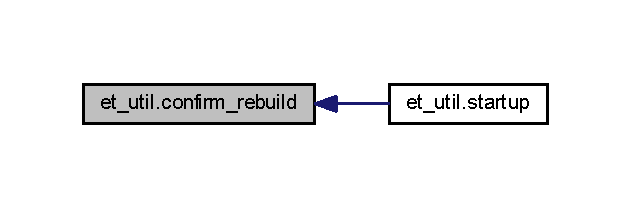
\includegraphics[width=303pt]{namespaceet__util_ad79d083c0b67b0c0aa1c3f9f247bf856_icgraph}
\end{center}
\end{figure}


\hypertarget{namespaceet__util_ac2422e9d685033121b1c6739352cf345}{}\index{et\+\_\+util@{et\+\_\+util}!convert\+\_\+precip@{convert\+\_\+precip}}
\index{convert\+\_\+precip@{convert\+\_\+precip}!et\+\_\+util@{et\+\_\+util}}
\subsubsection[{convert\+\_\+precip}]{\setlength{\rightskip}{0pt plus 5cm}def et\+\_\+util.\+convert\+\_\+precip (
\begin{DoxyParamCaption}
\item[{}]{df}
\end{DoxyParamCaption}
)}\label{namespaceet__util_ac2422e9d685033121b1c6739352cf345}


Definition at line 447 of file et\+\_\+util.\+py.



Here is the caller graph for this function\+:
\nopagebreak
\begin{figure}[H]
\begin{center}
\leavevmode
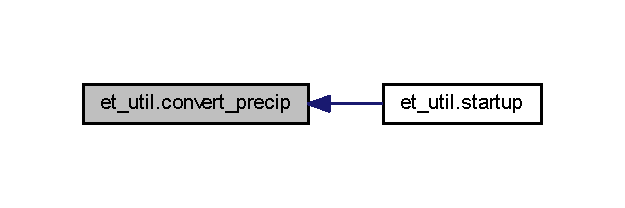
\includegraphics[width=300pt]{namespaceet__util_ac2422e9d685033121b1c6739352cf345_icgraph}
\end{center}
\end{figure}


\hypertarget{namespaceet__util_a45d34a2e8a980bed1bcf1c8d708399cc}{}\index{et\+\_\+util@{et\+\_\+util}!d\+\_\+met\+\_\+calcs@{d\+\_\+met\+\_\+calcs}}
\index{d\+\_\+met\+\_\+calcs@{d\+\_\+met\+\_\+calcs}!et\+\_\+util@{et\+\_\+util}}
\subsubsection[{d\+\_\+met\+\_\+calcs}]{\setlength{\rightskip}{0pt plus 5cm}def et\+\_\+util.\+d\+\_\+met\+\_\+calcs (
\begin{DoxyParamCaption}
\item[{}]{path\+\_\+out, }
\item[{}]{df\+\_\+m, }
\item[{}]{df\+\_\+r, }
\item[{}]{df\+\_\+e, }
\item[{}]{station, }
\item[{}]{make\+\_\+calc\+\_\+plots = {\ttfamily True}}
\end{DoxyParamCaption}
)}\label{namespaceet__util_a45d34a2e8a980bed1bcf1c8d708399cc}
\begin{DoxyVerb}Do met calcs for fortran program input.

:param df_m: Concatenated data logger met data over analysis interval
:param df_r: Concatenated data logger rad data over analysis interval
:param df_e: Concatenated data logger ec data over analysis interval
:param make_calc_plots: logical plot toggle
:return: df_out
\end{DoxyVerb}
\begin{DoxyVerb}print '#################################################'
print "From s_met_calcs, describe df_r:"
print df_r.describe()
print df_r.dtypes
print '#################################################'
\end{DoxyVerb}
 

Definition at line 1440 of file et\+\_\+util.\+py.



Here is the call graph for this function\+:\nopagebreak
\begin{figure}[H]
\begin{center}
\leavevmode
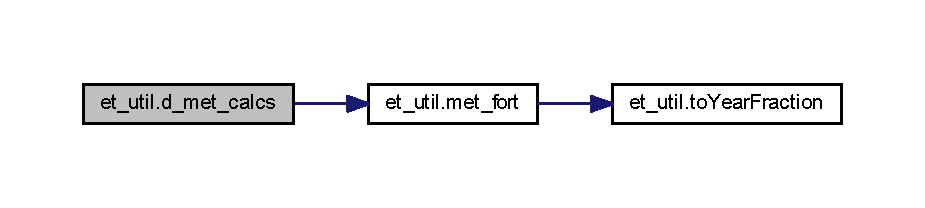
\includegraphics[width=350pt]{namespaceet__util_a45d34a2e8a980bed1bcf1c8d708399cc_cgraph}
\end{center}
\end{figure}


\hypertarget{namespaceet__util_a07507bce96a663ca49bd206aadc6272c}{}\index{et\+\_\+util@{et\+\_\+util}!df\+\_\+csv@{df\+\_\+csv}}
\index{df\+\_\+csv@{df\+\_\+csv}!et\+\_\+util@{et\+\_\+util}}
\subsubsection[{df\+\_\+csv}]{\setlength{\rightskip}{0pt plus 5cm}def et\+\_\+util.\+df\+\_\+csv (
\begin{DoxyParamCaption}
\item[{}]{df\+\_\+v, }
\item[{}]{fname, }
\item[{}]{df\+\_\+type, }
\item[{}]{df\+\_\+name = {\ttfamily \textquotesingle{}df\textquotesingle{}}, }
\item[{}]{echo = {\ttfamily False}, }
\item[{}]{index = {\ttfamily True}, }
\item[{}]{header = {\ttfamily True}}
\end{DoxyParamCaption}
)}\label{namespaceet__util_a07507bce96a663ca49bd206aadc6272c}
\begin{DoxyVerb}Output a DataFrame to csv file with option for feedback.

:rtype : object
:param df_v: DataFrame to write
:param fname: Filename (path) to write to.
:param df_type: Data type (met, ec, or rad)
:param df_name: Name to pass to echo_description
:param echo: Logical to print description to console
:param index: Logical to include df index in file (False for raw (all) ec data)
:param header: Logical to include header in file (False for raw (all) ec data)
:return: Nothing
\end{DoxyVerb}
 

Definition at line 1775 of file et\+\_\+util.\+py.



Here is the call graph for this function\+:\nopagebreak
\begin{figure}[H]
\begin{center}
\leavevmode
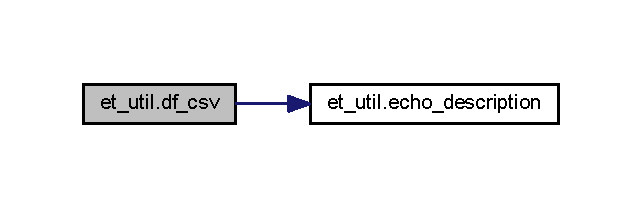
\includegraphics[width=308pt]{namespaceet__util_a07507bce96a663ca49bd206aadc6272c_cgraph}
\end{center}
\end{figure}


\hypertarget{namespaceet__util_abbaa0589af07e21f8a1d98515aafef03}{}\index{et\+\_\+util@{et\+\_\+util}!df\+\_\+dat@{df\+\_\+dat}}
\index{df\+\_\+dat@{df\+\_\+dat}!et\+\_\+util@{et\+\_\+util}}
\subsubsection[{df\+\_\+dat}]{\setlength{\rightskip}{0pt plus 5cm}def et\+\_\+util.\+df\+\_\+dat (
\begin{DoxyParamCaption}
\item[{}]{df\+\_\+v, }
\item[{}]{fname}
\end{DoxyParamCaption}
)}\label{namespaceet__util_abbaa0589af07e21f8a1d98515aafef03}


Orphan code functions. 

\begin{DoxyVerb}This doesn't do anything yet.
\end{DoxyVerb}
 

Definition at line 1819 of file et\+\_\+util.\+py.

\hypertarget{namespaceet__util_add60caac6c3d8333a58794a411891f57}{}\index{et\+\_\+util@{et\+\_\+util}!doy\+\_\+parser@{doy\+\_\+parser}}
\index{doy\+\_\+parser@{doy\+\_\+parser}!et\+\_\+util@{et\+\_\+util}}
\subsubsection[{doy\+\_\+parser}]{\setlength{\rightskip}{0pt plus 5cm}def et\+\_\+util.\+doy\+\_\+parser (
\begin{DoxyParamCaption}
\item[{}]{year, }
\item[{}]{doy, }
\item[{}]{time}
\end{DoxyParamCaption}
)}\label{namespaceet__util_add60caac6c3d8333a58794a411891f57}
\begin{DoxyVerb}Parse day of year from CR10X into datetime for read_csv.

:param year: 4-digit year
:param doy:  day of year
:param time: time as HHMM w/o leading zeros
:return: datetime variable

Dependants: read_s_ec read_d_ec, read_s_met, read_d_met
Internal Dependencies: None
External Dependencies: datetime, time
\end{DoxyVerb}
 

Definition at line 826 of file et\+\_\+util.\+py.

\hypertarget{namespaceet__util_a4fd6a305cc0207763b1d2386f9eeac84}{}\index{et\+\_\+util@{et\+\_\+util}!ec\+\_\+fort@{ec\+\_\+fort}}
\index{ec\+\_\+fort@{ec\+\_\+fort}!et\+\_\+util@{et\+\_\+util}}
\subsubsection[{ec\+\_\+fort}]{\setlength{\rightskip}{0pt plus 5cm}def et\+\_\+util.\+ec\+\_\+fort (
\begin{DoxyParamCaption}
\item[{}]{df\+\_\+ec}
\end{DoxyParamCaption}
)}\label{namespaceet__util_a4fd6a305cc0207763b1d2386f9eeac84}
\begin{DoxyVerb}Output ec data to fortran input file.

:param df_ec: DataFrame of ec data for fortran input
:return: Nothing, writes text file alldata.dat for fortran input
\end{DoxyVerb}
 

Definition at line 1689 of file et\+\_\+util.\+py.



Here is the call graph for this function\+:\nopagebreak
\begin{figure}[H]
\begin{center}
\leavevmode
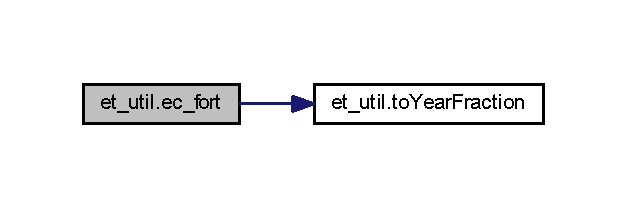
\includegraphics[width=301pt]{namespaceet__util_a4fd6a305cc0207763b1d2386f9eeac84_cgraph}
\end{center}
\end{figure}


\hypertarget{namespaceet__util_a15aa7ba554d08be6cbf6a674accfa16e}{}\index{et\+\_\+util@{et\+\_\+util}!echo\+\_\+description@{echo\+\_\+description}}
\index{echo\+\_\+description@{echo\+\_\+description}!et\+\_\+util@{et\+\_\+util}}
\subsubsection[{echo\+\_\+description}]{\setlength{\rightskip}{0pt plus 5cm}def et\+\_\+util.\+echo\+\_\+description (
\begin{DoxyParamCaption}
\item[{}]{df\+\_\+v, }
\item[{}]{fname = {\ttfamily \textquotesingle{}Dataframe\textquotesingle{}}, }
\item[{}]{df\+\_\+type = {\ttfamily \textquotesingle{}default\textquotesingle{}}, }
\item[{}]{df\+\_\+name = {\ttfamily \textquotesingle{}df\textquotesingle{}}}
\end{DoxyParamCaption}
)}\label{namespaceet__util_a15aa7ba554d08be6cbf6a674accfa16e}
\begin{DoxyVerb}Prints custom timeseries dataframe description with lengths and index names.
\end{DoxyVerb}
 

Definition at line 1795 of file et\+\_\+util.\+py.



Here is the caller graph for this function\+:
\nopagebreak
\begin{figure}[H]
\begin{center}
\leavevmode
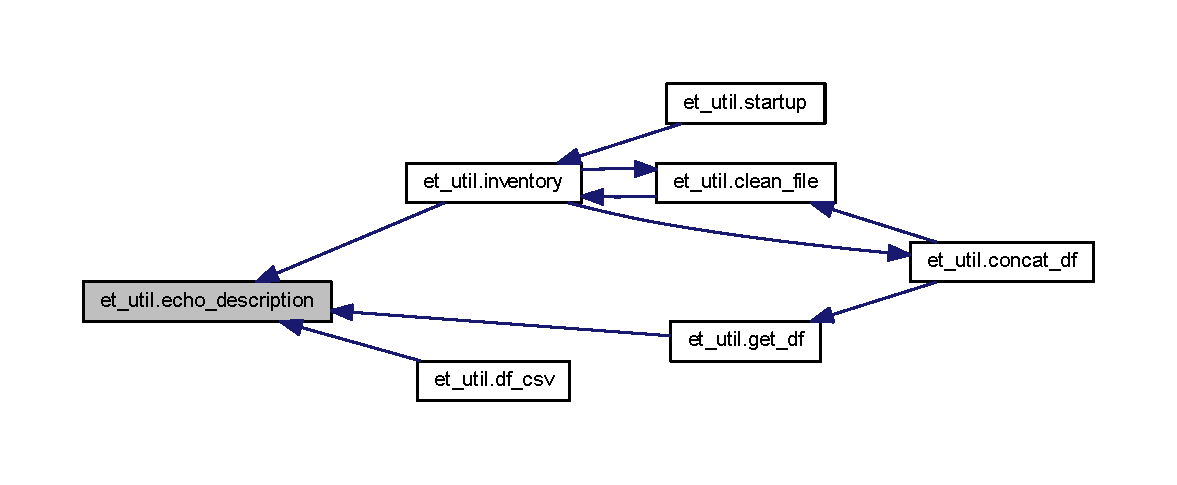
\includegraphics[width=350pt]{namespaceet__util_a15aa7ba554d08be6cbf6a674accfa16e_icgraph}
\end{center}
\end{figure}


\hypertarget{namespaceet__util_a15b819dcfa7f04be44839a9887e62c41}{}\index{et\+\_\+util@{et\+\_\+util}!gap@{gap}}
\index{gap@{gap}!et\+\_\+util@{et\+\_\+util}}
\subsubsection[{gap}]{\setlength{\rightskip}{0pt plus 5cm}def et\+\_\+util.\+gap (
\begin{DoxyParamCaption}
\item[{}]{path, }
\item[{}]{df0, }
\item[{}]{dtype, }
\item[{}]{make\+\_\+gap\+\_\+plots}
\end{DoxyParamCaption}
)}\label{namespaceet__util_a15b819dcfa7f04be44839a9887e62c41}
\begin{DoxyVerb}Catalog and plot time gaps in a time series DataFrame.

:param df0: Time series DataFrame to be checked for gaps.
:param dtype: Data file type (met, ec, rad)
:param make_gap_plots: logical
:return: df_gap - DataFrame of gap lengths and start times.

Other stuff after field list
\end{DoxyVerb}
 

Definition at line 996 of file et\+\_\+util.\+py.



Here is the call graph for this function\+:\nopagebreak
\begin{figure}[H]
\begin{center}
\leavevmode
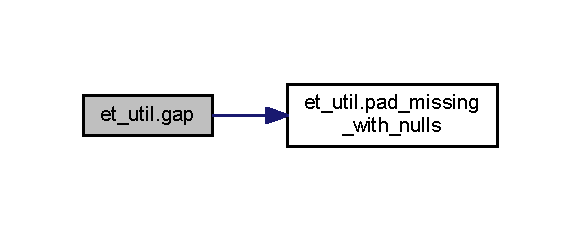
\includegraphics[width=279pt]{namespaceet__util_a15b819dcfa7f04be44839a9887e62c41_cgraph}
\end{center}
\end{figure}


\hypertarget{namespaceet__util_a86bdf627c5eafcab2d20a7d1ce75a1ed}{}\index{et\+\_\+util@{et\+\_\+util}!gap\+\_\+expand@{gap\+\_\+expand}}
\index{gap\+\_\+expand@{gap\+\_\+expand}!et\+\_\+util@{et\+\_\+util}}
\subsubsection[{gap\+\_\+expand}]{\setlength{\rightskip}{0pt plus 5cm}def et\+\_\+util.\+gap\+\_\+expand (
\begin{DoxyParamCaption}
\item[{}]{path\+\_\+out, }
\item[{}]{column}
\end{DoxyParamCaption}
)}\label{namespaceet__util_a86bdf627c5eafcab2d20a7d1ce75a1ed}
\begin{DoxyVerb}Use gap file to build even interval time series of gap lengths
\end{DoxyVerb}
 

Definition at line 1067 of file et\+\_\+util.\+py.



Here is the caller graph for this function\+:\nopagebreak
\begin{figure}[H]
\begin{center}
\leavevmode
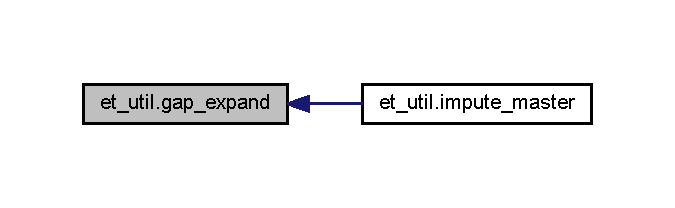
\includegraphics[width=324pt]{namespaceet__util_a86bdf627c5eafcab2d20a7d1ce75a1ed_icgraph}
\end{center}
\end{figure}


\hypertarget{namespaceet__util_a8013dc0897f9430ae8f354ba094b9fbd}{}\index{et\+\_\+util@{et\+\_\+util}!get\+\_\+df@{get\+\_\+df}}
\index{get\+\_\+df@{get\+\_\+df}!et\+\_\+util@{et\+\_\+util}}
\subsubsection[{get\+\_\+df}]{\setlength{\rightskip}{0pt plus 5cm}def et\+\_\+util.\+get\+\_\+df (
\begin{DoxyParamCaption}
\item[{}]{fname, }
\item[{}]{df\+\_\+type, }
\item[{}]{out\+\_\+form, }
\item[{}]{station, }
\item[{}]{echo\+\_\+get}
\end{DoxyParamCaption}
)}\label{namespaceet__util_a8013dc0897f9430ae8f354ba094b9fbd}
\begin{DoxyVerb}"Call correct Campbell read function for station and data type and print feedback"

:param fname: file path
:param df_type: Datafile type (ec, met, rad)
:param station: Starkey or Dead River
:param echo_get: enable or disable print feedback
:return: DataFrame of datafile

Dependants: concat_df
Internal Dependencies:none
External Dependencies:pandas
\end{DoxyVerb}
 

Definition at line 562 of file et\+\_\+util.\+py.



Here is the call graph for this function\+:\nopagebreak
\begin{figure}[H]
\begin{center}
\leavevmode
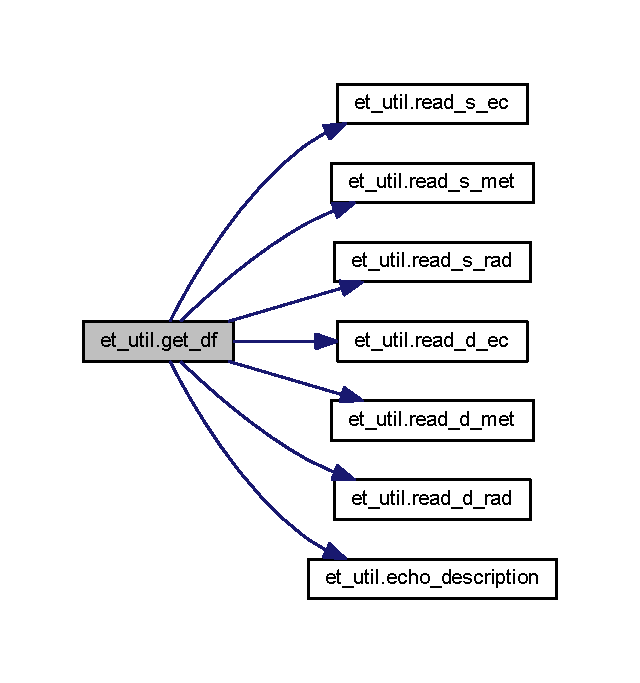
\includegraphics[width=307pt]{namespaceet__util_a8013dc0897f9430ae8f354ba094b9fbd_cgraph}
\end{center}
\end{figure}




Here is the caller graph for this function\+:
\nopagebreak
\begin{figure}[H]
\begin{center}
\leavevmode
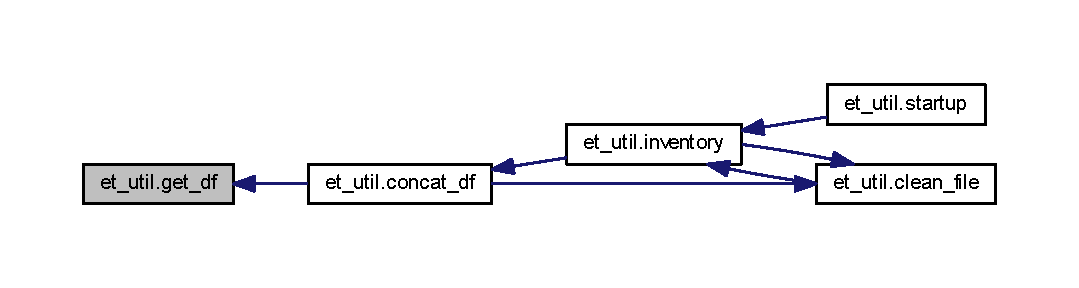
\includegraphics[width=350pt]{namespaceet__util_a8013dc0897f9430ae8f354ba094b9fbd_icgraph}
\end{center}
\end{figure}


\hypertarget{namespaceet__util_a3c3ae2439b3b5337237d456cb4366028}{}\index{et\+\_\+util@{et\+\_\+util}!get\+\_\+file\+\_\+times@{get\+\_\+file\+\_\+times}}
\index{get\+\_\+file\+\_\+times@{get\+\_\+file\+\_\+times}!et\+\_\+util@{et\+\_\+util}}
\subsubsection[{get\+\_\+file\+\_\+times}]{\setlength{\rightskip}{0pt plus 5cm}def et\+\_\+util.\+get\+\_\+file\+\_\+times (
\begin{DoxyParamCaption}
\item[{}]{config}
\end{DoxyParamCaption}
)}\label{namespaceet__util_a3c3ae2439b3b5337237d456cb4366028}
\begin{DoxyVerb}Reads Configuration.txt and gets archive start and end times.

:return: file_times list

Dependents: main
External Dependencies: datetime
\end{DoxyVerb}
 

Definition at line 172 of file et\+\_\+util.\+py.



Here is the caller graph for this function\+:
\nopagebreak
\begin{figure}[H]
\begin{center}
\leavevmode
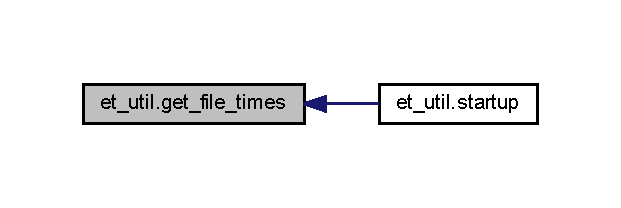
\includegraphics[width=298pt]{namespaceet__util_a3c3ae2439b3b5337237d456cb4366028_icgraph}
\end{center}
\end{figure}


\hypertarget{namespaceet__util_abf296bc00b589318395becdb4aa3f89d}{}\index{et\+\_\+util@{et\+\_\+util}!impute\+\_\+master@{impute\+\_\+master}}
\index{impute\+\_\+master@{impute\+\_\+master}!et\+\_\+util@{et\+\_\+util}}
\subsubsection[{impute\+\_\+master}]{\setlength{\rightskip}{0pt plus 5cm}def et\+\_\+util.\+impute\+\_\+master (
\begin{DoxyParamCaption}
\item[{}]{path\+\_\+out, }
\item[{}]{df}
\end{DoxyParamCaption}
)}\label{namespaceet__util_abf296bc00b589318395becdb4aa3f89d}
\begin{DoxyVerb}Control missing value imputation.  Calls impute_strata.

:param path_out:
:param df:
:return:
\end{DoxyVerb}
\begin{DoxyVerb}response = ' '  # just to make pyCharm happy.
while True:
    prompt_message = 'Make Histograms (Y/N)? '
    response = raw_input(prompt_message).upper()
    if response in ['Y', 'N']:
        break
    else:
        print "Not a valid entry"
if response == 'Y':
    df.hist()
    #df.plot(kind='hist')
    plt.show()\end{DoxyVerb}
 

Definition at line 1112 of file et\+\_\+util.\+py.



Here is the call graph for this function\+:\nopagebreak
\begin{figure}[H]
\begin{center}
\leavevmode
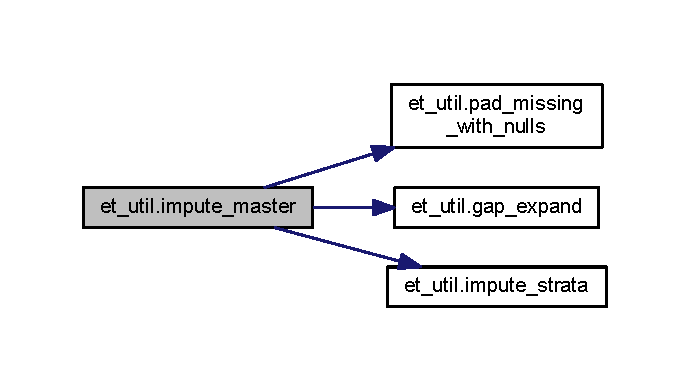
\includegraphics[width=331pt]{namespaceet__util_abf296bc00b589318395becdb4aa3f89d_cgraph}
\end{center}
\end{figure}


\hypertarget{namespaceet__util_ae6b0b0285532d32dd9d5d2b42c7f6043}{}\index{et\+\_\+util@{et\+\_\+util}!impute\+\_\+simple@{impute\+\_\+simple}}
\index{impute\+\_\+simple@{impute\+\_\+simple}!et\+\_\+util@{et\+\_\+util}}
\subsubsection[{impute\+\_\+simple}]{\setlength{\rightskip}{0pt plus 5cm}def et\+\_\+util.\+impute\+\_\+simple (
\begin{DoxyParamCaption}
\item[{}]{path\+\_\+out, }
\item[{}]{df, }
\item[{}]{dtype, }
\item[{}]{print\+\_\+flag}
\end{DoxyParamCaption}
)}\label{namespaceet__util_ae6b0b0285532d32dd9d5d2b42c7f6043}
\begin{DoxyVerb}Function to impute entire missing records"

:param df: Dataframe to impute.
:param print_flag: Flag to indicate if diagnostic files should be printed
:return: dataframe with imputed values and an added flag column
\end{DoxyVerb}
 

Definition at line 1229 of file et\+\_\+util.\+py.

\hypertarget{namespaceet__util_ad991b40a8a99a7e5384f3bdfb1258af5}{}\index{et\+\_\+util@{et\+\_\+util}!impute\+\_\+strata@{impute\+\_\+strata}}
\index{impute\+\_\+strata@{impute\+\_\+strata}!et\+\_\+util@{et\+\_\+util}}
\subsubsection[{impute\+\_\+strata}]{\setlength{\rightskip}{0pt plus 5cm}def et\+\_\+util.\+impute\+\_\+strata (
\begin{DoxyParamCaption}
\item[{}]{path\+\_\+out, }
\item[{}]{df, }
\item[{}]{df\+\_\+month\+\_\+mn, }
\item[{}]{column, }
\item[{}]{mask}
\end{DoxyParamCaption}
)}\label{namespaceet__util_ad991b40a8a99a7e5384f3bdfb1258af5}
\begin{DoxyVerb}Fill one column that has missing data from a dataframe using methods based on length missing.

:param path_out: where to write check files
:param df: dataframe to impute
:param df_month_mn: monthly means
:param column: current column name
:param mask: even interval series of missing lengths for column
:return: dataframe
\end{DoxyVerb}
 

Definition at line 1190 of file et\+\_\+util.\+py.



Here is the caller graph for this function\+:\nopagebreak
\begin{figure}[H]
\begin{center}
\leavevmode
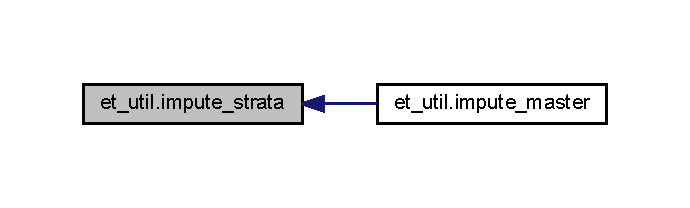
\includegraphics[width=331pt]{namespaceet__util_ad991b40a8a99a7e5384f3bdfb1258af5_icgraph}
\end{center}
\end{figure}


\hypertarget{namespaceet__util_ad14756ce8dfea7ab6da605eb2a34af45}{}\index{et\+\_\+util@{et\+\_\+util}!inventory@{inventory}}
\index{inventory@{inventory}!et\+\_\+util@{et\+\_\+util}}
\subsubsection[{inventory}]{\setlength{\rightskip}{0pt plus 5cm}def et\+\_\+util.\+inventory (
\begin{DoxyParamCaption}
\item[{}]{path\+\_\+in, }
\item[{}]{path\+\_\+out, }
\item[{}]{path\+\_\+temp, }
\item[{}]{station, }
\item[{}]{station\+\_\+prefix, }
\item[{}]{analysis\+\_\+start, }
\item[{}]{combined\+\_\+echo, }
\item[{}]{echo\+\_\+get}
\end{DoxyParamCaption}
)}\label{namespaceet__util_ad14756ce8dfea7ab6da605eb2a34af45}


Definition at line 235 of file et\+\_\+util.\+py.



Here is the call graph for this function\+:
\nopagebreak
\begin{figure}[H]
\begin{center}
\leavevmode
\includegraphics[width=350pt]{namespaceet__util_ad14756ce8dfea7ab6da605eb2a34af45_cgraph}
\end{center}
\end{figure}




Here is the caller graph for this function\+:
\nopagebreak
\begin{figure}[H]
\begin{center}
\leavevmode
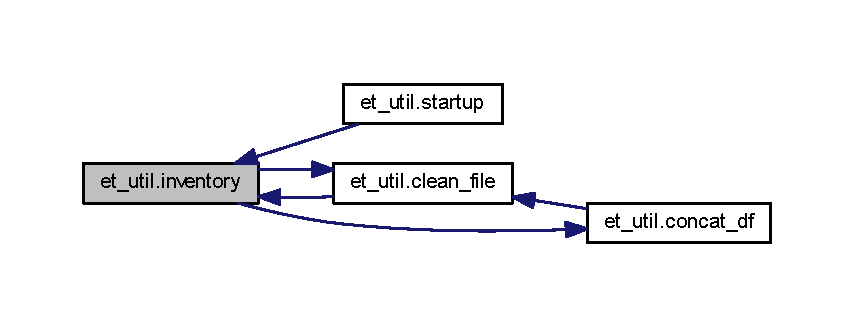
\includegraphics[width=350pt]{namespaceet__util_ad14756ce8dfea7ab6da605eb2a34af45_icgraph}
\end{center}
\end{figure}


\hypertarget{namespaceet__util_a3331dc365022196889cfcd3fa3cca3b2}{}\index{et\+\_\+util@{et\+\_\+util}!join\+\_\+and\+\_\+delete@{join\+\_\+and\+\_\+delete}}
\index{join\+\_\+and\+\_\+delete@{join\+\_\+and\+\_\+delete}!et\+\_\+util@{et\+\_\+util}}
\subsubsection[{join\+\_\+and\+\_\+delete}]{\setlength{\rightskip}{0pt plus 5cm}def et\+\_\+util.\+join\+\_\+and\+\_\+delete (
\begin{DoxyParamCaption}
\item[{}]{df, }
\item[{}]{path\+\_\+out, }
\item[{}]{fname, }
\item[{}]{delete\+\_\+list}
\end{DoxyParamCaption}
)}\label{namespaceet__util_a3331dc365022196889cfcd3fa3cca3b2}


Definition at line 482 of file et\+\_\+util.\+py.



Here is the caller graph for this function\+:
\nopagebreak
\begin{figure}[H]
\begin{center}
\leavevmode
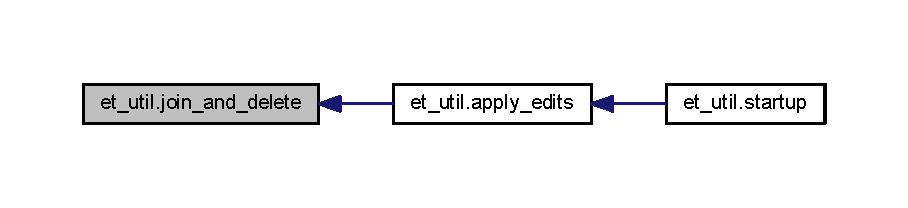
\includegraphics[width=350pt]{namespaceet__util_a3331dc365022196889cfcd3fa3cca3b2_icgraph}
\end{center}
\end{figure}


\hypertarget{namespaceet__util_a241e2fa8182c03412e519a4c6431d29b}{}\index{et\+\_\+util@{et\+\_\+util}!met\+\_\+filter@{met\+\_\+filter}}
\index{met\+\_\+filter@{met\+\_\+filter}!et\+\_\+util@{et\+\_\+util}}
\subsubsection[{met\+\_\+filter}]{\setlength{\rightskip}{0pt plus 5cm}def et\+\_\+util.\+met\+\_\+filter (
\begin{DoxyParamCaption}
\item[{}]{df\+\_\+met, }
\item[{}]{station}
\end{DoxyParamCaption}
)}\label{namespaceet__util_a241e2fa8182c03412e519a4c6431d29b}


Definition at line 417 of file et\+\_\+util.\+py.



Here is the caller graph for this function\+:
\nopagebreak
\begin{figure}[H]
\begin{center}
\leavevmode
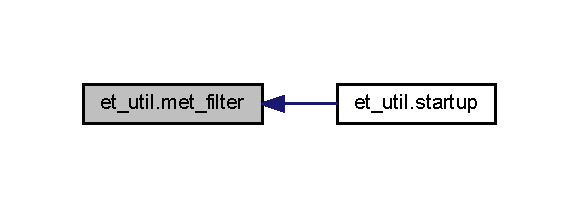
\includegraphics[width=278pt]{namespaceet__util_a241e2fa8182c03412e519a4c6431d29b_icgraph}
\end{center}
\end{figure}


\hypertarget{namespaceet__util_a04161955cfa0207847c92471361582ae}{}\index{et\+\_\+util@{et\+\_\+util}!met\+\_\+fort@{met\+\_\+fort}}
\index{met\+\_\+fort@{met\+\_\+fort}!et\+\_\+util@{et\+\_\+util}}
\subsubsection[{met\+\_\+fort}]{\setlength{\rightskip}{0pt plus 5cm}def et\+\_\+util.\+met\+\_\+fort (
\begin{DoxyParamCaption}
\item[{}]{path\+\_\+out, }
\item[{}]{df\+\_\+out, }
\item[{}]{station}
\end{DoxyParamCaption}
)}\label{namespaceet__util_a04161955cfa0207847c92471361582ae}
\begin{DoxyVerb}Output alldata.prn for fortran met data input.

:param path_out: Output directory relative to program location
:param df_out: Timeseries DataFrame of output variables
:return: nothing
\end{DoxyVerb}
 

Definition at line 1597 of file et\+\_\+util.\+py.



Here is the call graph for this function\+:\nopagebreak
\begin{figure}[H]
\begin{center}
\leavevmode
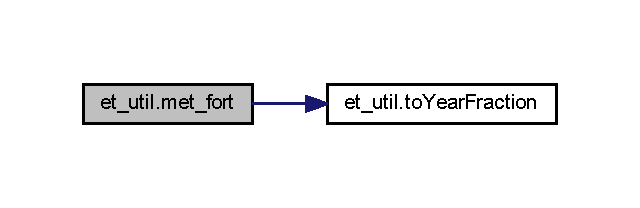
\includegraphics[width=307pt]{namespaceet__util_a04161955cfa0207847c92471361582ae_cgraph}
\end{center}
\end{figure}




Here is the caller graph for this function\+:\nopagebreak
\begin{figure}[H]
\begin{center}
\leavevmode
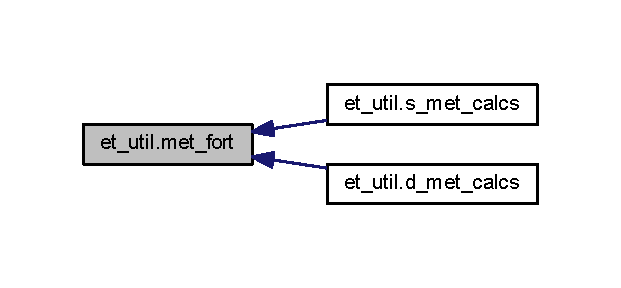
\includegraphics[width=298pt]{namespaceet__util_a04161955cfa0207847c92471361582ae_icgraph}
\end{center}
\end{figure}


\hypertarget{namespaceet__util_ad1b21b5159cbb574e683156c7870b06d}{}\index{et\+\_\+util@{et\+\_\+util}!missnaec@{missnaec}}
\index{missnaec@{missnaec}!et\+\_\+util@{et\+\_\+util}}
\subsubsection[{missnaec}]{\setlength{\rightskip}{0pt plus 5cm}def et\+\_\+util.\+missnaec (
\begin{DoxyParamCaption}
\item[{}]{df}
\end{DoxyParamCaption}
)}\label{namespaceet__util_ad1b21b5159cbb574e683156c7870b06d}
\begin{DoxyVerb}Replace values out of bounds with missing (should count them).

:param df: Input DataFrame
:return: df - Output DataFrame

Immediately obsolete but structure may be useful again:
\end{DoxyVerb}
 

Definition at line 1835 of file et\+\_\+util.\+py.

\hypertarget{namespaceet__util_a9d53464743ec890e7b0a9d367d09a6ad}{}\index{et\+\_\+util@{et\+\_\+util}!pad\+\_\+missing\+\_\+with\+\_\+nulls@{pad\+\_\+missing\+\_\+with\+\_\+nulls}}
\index{pad\+\_\+missing\+\_\+with\+\_\+nulls@{pad\+\_\+missing\+\_\+with\+\_\+nulls}!et\+\_\+util@{et\+\_\+util}}
\subsubsection[{pad\+\_\+missing\+\_\+with\+\_\+nulls}]{\setlength{\rightskip}{0pt plus 5cm}def et\+\_\+util.\+pad\+\_\+missing\+\_\+with\+\_\+nulls (
\begin{DoxyParamCaption}
\item[{}]{df\+\_\+pad, }
\item[{}]{dtype}
\end{DoxyParamCaption}
)}\label{namespaceet__util_a9d53464743ec890e7b0a9d367d09a6ad}
\begin{DoxyVerb}Insert blank rows for missing 30min timestamps. Used by gap and impute.

:param df_pad: dataframe to pad
:param dtype:  type of data in dataframe
:return: padded dataframe df_pad
\end{DoxyVerb}
 

Definition at line 972 of file et\+\_\+util.\+py.



Here is the caller graph for this function\+:\nopagebreak
\begin{figure}[H]
\begin{center}
\leavevmode
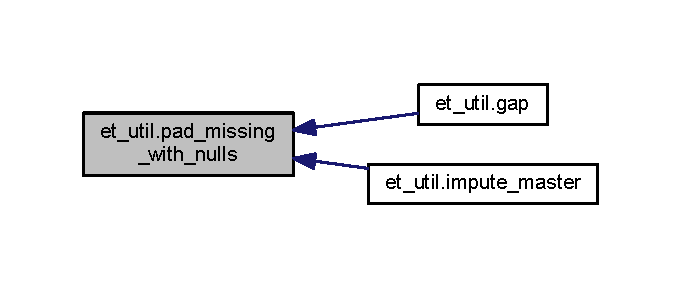
\includegraphics[width=327pt]{namespaceet__util_a9d53464743ec890e7b0a9d367d09a6ad_icgraph}
\end{center}
\end{figure}


\hypertarget{namespaceet__util_a566ff749c2a2c113c58d24649251bd5b}{}\index{et\+\_\+util@{et\+\_\+util}!read\+\_\+\+C\+Rten\+X\+\_\+file@{read\+\_\+\+C\+Rten\+X\+\_\+file}}
\index{read\+\_\+\+C\+Rten\+X\+\_\+file@{read\+\_\+\+C\+Rten\+X\+\_\+file}!et\+\_\+util@{et\+\_\+util}}
\subsubsection[{read\+\_\+\+C\+Rten\+X\+\_\+file}]{\setlength{\rightskip}{0pt plus 5cm}def et\+\_\+util.\+read\+\_\+\+C\+Rten\+X\+\_\+file (
\begin{DoxyParamCaption}
\item[{}]{path, }
\item[{}]{fname, }
\item[{}]{df\+\_\+type}
\end{DoxyParamCaption}
)}\label{namespaceet__util_a566ff749c2a2c113c58d24649251bd5b}
\begin{DoxyVerb}Return dict entry of CR10X file time span.

:param path: file path
:param fname: file name (stored in output data)
:param df_type: datafile type (met or ec)
:return: DataFrame entry of begin and end date times for file.

Dependants: main
Internal Dependencies:none
External Dependencies:pandas
\end{DoxyVerb}
 

Definition at line 896 of file et\+\_\+util.\+py.



Here is the caller graph for this function\+:
\nopagebreak
\begin{figure}[H]
\begin{center}
\leavevmode
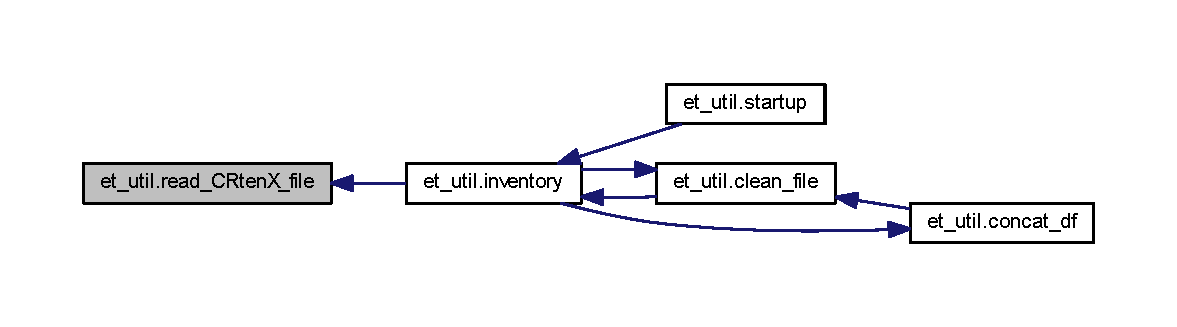
\includegraphics[width=350pt]{namespaceet__util_a566ff749c2a2c113c58d24649251bd5b_icgraph}
\end{center}
\end{figure}


\hypertarget{namespaceet__util_af15d3c41901948dbb10f0c796cb6ed5b}{}\index{et\+\_\+util@{et\+\_\+util}!read\+\_\+\+C\+Rthousand\+\_\+file@{read\+\_\+\+C\+Rthousand\+\_\+file}}
\index{read\+\_\+\+C\+Rthousand\+\_\+file@{read\+\_\+\+C\+Rthousand\+\_\+file}!et\+\_\+util@{et\+\_\+util}}
\subsubsection[{read\+\_\+\+C\+Rthousand\+\_\+file}]{\setlength{\rightskip}{0pt plus 5cm}def et\+\_\+util.\+read\+\_\+\+C\+Rthousand\+\_\+file (
\begin{DoxyParamCaption}
\item[{}]{f, }
\item[{}]{fname}
\end{DoxyParamCaption}
)}\label{namespaceet__util_af15d3c41901948dbb10f0c796cb6ed5b}
\begin{DoxyVerb}Read CR1000 file time spans.

Reads file 'f' from folder 'path' as a pandas dataframe.
Returns first and last timestamp with filename as key.

:param f: file path
:param fname: file name (stored in output data)
:return: DataFrame entry of begin and end date times for file.

Dependants: main
Internal Dependencies:none
External Dependencies:pandas
\end{DoxyVerb}
 

Definition at line 934 of file et\+\_\+util.\+py.



Here is the caller graph for this function\+:
\nopagebreak
\begin{figure}[H]
\begin{center}
\leavevmode
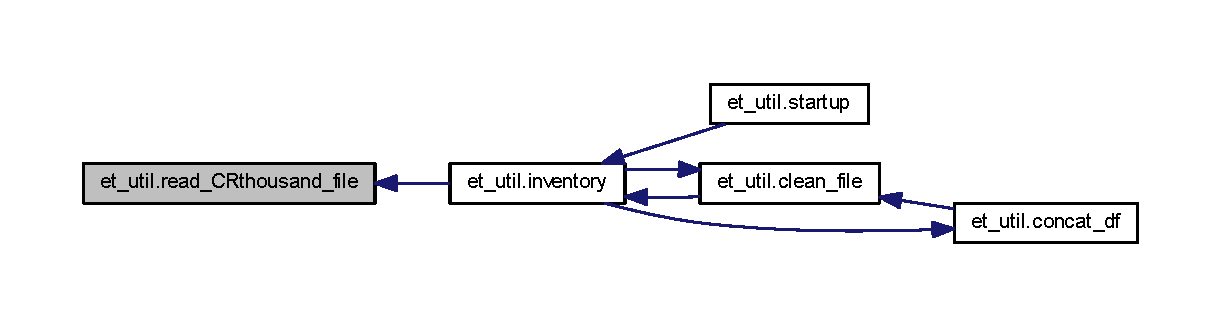
\includegraphics[width=350pt]{namespaceet__util_af15d3c41901948dbb10f0c796cb6ed5b_icgraph}
\end{center}
\end{figure}


\hypertarget{namespaceet__util_a5cda9dc3d34bdd80d01b977e805f4b04}{}\index{et\+\_\+util@{et\+\_\+util}!read\+\_\+d\+\_\+ec@{read\+\_\+d\+\_\+ec}}
\index{read\+\_\+d\+\_\+ec@{read\+\_\+d\+\_\+ec}!et\+\_\+util@{et\+\_\+util}}
\subsubsection[{read\+\_\+d\+\_\+ec}]{\setlength{\rightskip}{0pt plus 5cm}def et\+\_\+util.\+read\+\_\+d\+\_\+ec (
\begin{DoxyParamCaption}
\item[{}]{f, }
\item[{}]{out\+\_\+form = {\ttfamily \textquotesingle{}csv\textquotesingle{}}}
\end{DoxyParamCaption}
)}\label{namespaceet__util_a5cda9dc3d34bdd80d01b977e805f4b04}
\begin{DoxyVerb}Read Dead River ec CR10X file two ways depending on purpose.
   Keeps selected variables for analysis.

:param f: file path
:return: DataFrame of CR10X datafile with selected variables

Dependants: get_df - helper function
Internal Dependencies: doy_parser
External Dependencies:pandas
\end{DoxyVerb}
 

Definition at line 666 of file et\+\_\+util.\+py.



Here is the caller graph for this function\+:
\nopagebreak
\begin{figure}[H]
\begin{center}
\leavevmode
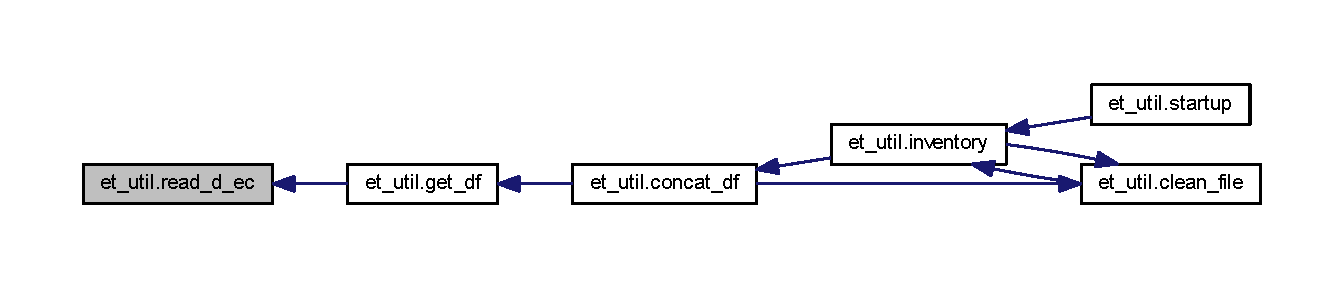
\includegraphics[width=350pt]{namespaceet__util_a5cda9dc3d34bdd80d01b977e805f4b04_icgraph}
\end{center}
\end{figure}


\hypertarget{namespaceet__util_aa20b5ae88dbfb272ae5e7f53f4678358}{}\index{et\+\_\+util@{et\+\_\+util}!read\+\_\+d\+\_\+met@{read\+\_\+d\+\_\+met}}
\index{read\+\_\+d\+\_\+met@{read\+\_\+d\+\_\+met}!et\+\_\+util@{et\+\_\+util}}
\subsubsection[{read\+\_\+d\+\_\+met}]{\setlength{\rightskip}{0pt plus 5cm}def et\+\_\+util.\+read\+\_\+d\+\_\+met (
\begin{DoxyParamCaption}
\item[{}]{f}
\end{DoxyParamCaption}
)}\label{namespaceet__util_aa20b5ae88dbfb272ae5e7f53f4678358}
\begin{DoxyVerb}Read Dead River met CR10X file two ways depending on purpose.
Keeps selected variables for analysis.

:param f: file path
:return: DataFrame of CR10X datafile with selected variables

Dependants: get_df - helper function
Internal Dependencies: doy_parser
External Dependencies:pandas
\end{DoxyVerb}
 

Definition at line 752 of file et\+\_\+util.\+py.



Here is the caller graph for this function\+:
\nopagebreak
\begin{figure}[H]
\begin{center}
\leavevmode
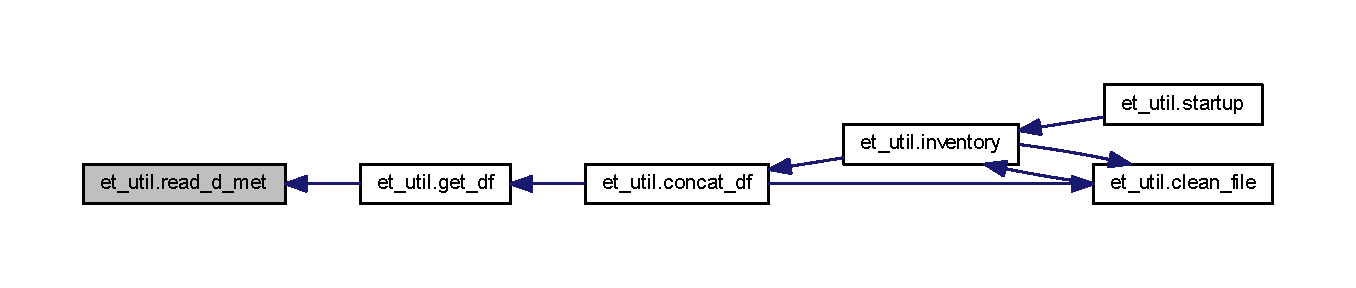
\includegraphics[width=350pt]{namespaceet__util_aa20b5ae88dbfb272ae5e7f53f4678358_icgraph}
\end{center}
\end{figure}


\hypertarget{namespaceet__util_a76d5a5c19f0e86b9ab70c0957827c260}{}\index{et\+\_\+util@{et\+\_\+util}!read\+\_\+d\+\_\+rad@{read\+\_\+d\+\_\+rad}}
\index{read\+\_\+d\+\_\+rad@{read\+\_\+d\+\_\+rad}!et\+\_\+util@{et\+\_\+util}}
\subsubsection[{read\+\_\+d\+\_\+rad}]{\setlength{\rightskip}{0pt plus 5cm}def et\+\_\+util.\+read\+\_\+d\+\_\+rad (
\begin{DoxyParamCaption}
\item[{}]{f}
\end{DoxyParamCaption}
)}\label{namespaceet__util_a76d5a5c19f0e86b9ab70c0957827c260}
\begin{DoxyVerb}Read Dead River met CR10X file.
Keeps selected variables for analysis.

:param f: file path
:return: DataFrame of CR10X datafile with selected variables

Dependants: get_df - helper function
Internal Dependencies: doy_parser
External Dependencies:pandas
\end{DoxyVerb}
 

Definition at line 802 of file et\+\_\+util.\+py.



Here is the caller graph for this function\+:
\nopagebreak
\begin{figure}[H]
\begin{center}
\leavevmode
\includegraphics[width=350pt]{namespaceet__util_a76d5a5c19f0e86b9ab70c0957827c260_icgraph}
\end{center}
\end{figure}


\hypertarget{namespaceet__util_adf3e6bef75b663226a9c118684f91689}{}\index{et\+\_\+util@{et\+\_\+util}!read\+\_\+files@{read\+\_\+files}}
\index{read\+\_\+files@{read\+\_\+files}!et\+\_\+util@{et\+\_\+util}}
\subsubsection[{read\+\_\+files}]{\setlength{\rightskip}{0pt plus 5cm}def et\+\_\+util.\+read\+\_\+files (
\begin{DoxyParamCaption}
\item[{}]{path\+\_\+out}
\end{DoxyParamCaption}
)}\label{namespaceet__util_adf3e6bef75b663226a9c118684f91689}


Definition at line 498 of file et\+\_\+util.\+py.



Here is the call graph for this function\+:\nopagebreak
\begin{figure}[H]
\begin{center}
\leavevmode
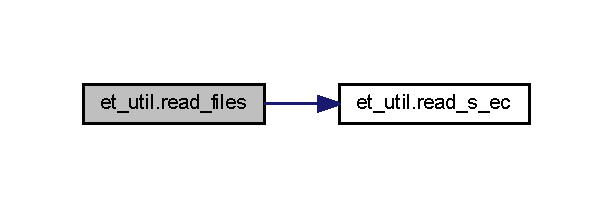
\includegraphics[width=294pt]{namespaceet__util_adf3e6bef75b663226a9c118684f91689_cgraph}
\end{center}
\end{figure}




Here is the caller graph for this function\+:
\nopagebreak
\begin{figure}[H]
\begin{center}
\leavevmode
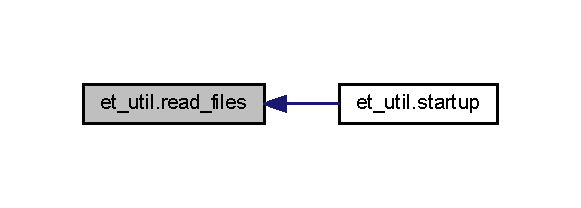
\includegraphics[width=279pt]{namespaceet__util_adf3e6bef75b663226a9c118684f91689_icgraph}
\end{center}
\end{figure}


\hypertarget{namespaceet__util_a7535fb2ada235d852a05717bdd6d67a9}{}\index{et\+\_\+util@{et\+\_\+util}!read\+\_\+s\+\_\+ec@{read\+\_\+s\+\_\+ec}}
\index{read\+\_\+s\+\_\+ec@{read\+\_\+s\+\_\+ec}!et\+\_\+util@{et\+\_\+util}}
\subsubsection[{read\+\_\+s\+\_\+ec}]{\setlength{\rightskip}{0pt plus 5cm}def et\+\_\+util.\+read\+\_\+s\+\_\+ec (
\begin{DoxyParamCaption}
\item[{}]{f, }
\item[{}]{out\+\_\+form = {\ttfamily \textquotesingle{}csv\textquotesingle{}}}
\end{DoxyParamCaption}
)}\label{namespaceet__util_a7535fb2ada235d852a05717bdd6d67a9}
\begin{DoxyVerb}Read Starkey ec CR10X file two ways depending on purpose.
Keeps all variables for 'non-csv' option.  Use for building input file for fortran.

:param f: file path
:param out_form: destination output type (csv drops extraneous variables)
:return: DataFrame of CR10X datafile with either selected variables or all

Dependants: get_df - helper function
Internal Dependencies: doy_parser
External Dependencies:pandas
\end{DoxyVerb}
 

Definition at line 603 of file et\+\_\+util.\+py.



Here is the caller graph for this function\+:
\nopagebreak
\begin{figure}[H]
\begin{center}
\leavevmode
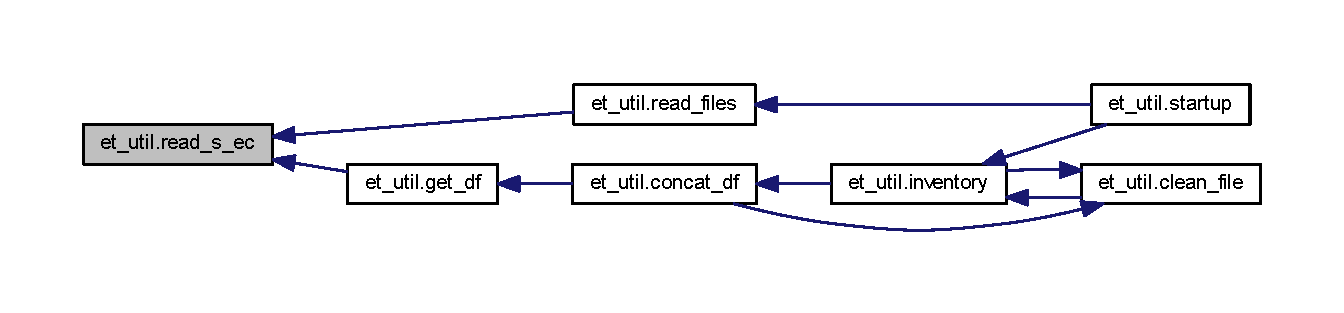
\includegraphics[width=350pt]{namespaceet__util_a7535fb2ada235d852a05717bdd6d67a9_icgraph}
\end{center}
\end{figure}


\hypertarget{namespaceet__util_a5cfb9371164d33036c4d3ec9f7a80e88}{}\index{et\+\_\+util@{et\+\_\+util}!read\+\_\+s\+\_\+met@{read\+\_\+s\+\_\+met}}
\index{read\+\_\+s\+\_\+met@{read\+\_\+s\+\_\+met}!et\+\_\+util@{et\+\_\+util}}
\subsubsection[{read\+\_\+s\+\_\+met}]{\setlength{\rightskip}{0pt plus 5cm}def et\+\_\+util.\+read\+\_\+s\+\_\+met (
\begin{DoxyParamCaption}
\item[{}]{f}
\end{DoxyParamCaption}
)}\label{namespaceet__util_a5cfb9371164d33036c4d3ec9f7a80e88}
\begin{DoxyVerb}Read Starkey met CR10X file two ways depending on purpose.
Keeps selected variables for analysis.

:param f: file path
:return: DataFrame of CR10X datafile with selected variables

Dependants: get_df - helper function
Internal Dependencies: doy_parser
External Dependencies:pandas
\end{DoxyVerb}
 

Definition at line 721 of file et\+\_\+util.\+py.



Here is the caller graph for this function\+:
\nopagebreak
\begin{figure}[H]
\begin{center}
\leavevmode
\includegraphics[width=350pt]{namespaceet__util_a5cfb9371164d33036c4d3ec9f7a80e88_icgraph}
\end{center}
\end{figure}


\hypertarget{namespaceet__util_a37255b034ed791b14cb66dc5df649a3f}{}\index{et\+\_\+util@{et\+\_\+util}!read\+\_\+s\+\_\+rad@{read\+\_\+s\+\_\+rad}}
\index{read\+\_\+s\+\_\+rad@{read\+\_\+s\+\_\+rad}!et\+\_\+util@{et\+\_\+util}}
\subsubsection[{read\+\_\+s\+\_\+rad}]{\setlength{\rightskip}{0pt plus 5cm}def et\+\_\+util.\+read\+\_\+s\+\_\+rad (
\begin{DoxyParamCaption}
\item[{}]{f}
\end{DoxyParamCaption}
)}\label{namespaceet__util_a37255b034ed791b14cb66dc5df649a3f}
\begin{DoxyVerb}Read Starkey CR1000 datafile of 4-comp radiometer.

:param f: file path
:return: DataFrame of 4-comp radiometer data.

Dependants: get_df - helper function
Internal Dependencies: doy_parser
External Dependencies:pandas
\end{DoxyVerb}
 

Definition at line 783 of file et\+\_\+util.\+py.



Here is the caller graph for this function\+:
\nopagebreak
\begin{figure}[H]
\begin{center}
\leavevmode
\includegraphics[width=350pt]{namespaceet__util_a37255b034ed791b14cb66dc5df649a3f_icgraph}
\end{center}
\end{figure}


\hypertarget{namespaceet__util_a28b3adad3d77922fccf7a1d77dd3adda}{}\index{et\+\_\+util@{et\+\_\+util}!s\+\_\+met\+\_\+calcs@{s\+\_\+met\+\_\+calcs}}
\index{s\+\_\+met\+\_\+calcs@{s\+\_\+met\+\_\+calcs}!et\+\_\+util@{et\+\_\+util}}
\subsubsection[{s\+\_\+met\+\_\+calcs}]{\setlength{\rightskip}{0pt plus 5cm}def et\+\_\+util.\+s\+\_\+met\+\_\+calcs (
\begin{DoxyParamCaption}
\item[{}]{path\+\_\+out, }
\item[{}]{df\+\_\+m, }
\item[{}]{df\+\_\+r, }
\item[{}]{df\+\_\+e, }
\item[{}]{station, }
\item[{}]{make\+\_\+calc\+\_\+plots = {\ttfamily True}}
\end{DoxyParamCaption}
)}\label{namespaceet__util_a28b3adad3d77922fccf7a1d77dd3adda}
\begin{DoxyVerb}Do met calcs for fortran program input.

:param path_out: Output directory relative to program folder
:param df_m: Concatenated data logger met data over analysis interval
:param df_r: Concatenated data logger rad data over analysis interval
:param df_e: Concatenated data logger ec data over analysis interval
:param station: Placeholder for eventual refactor
:param make_calc_plots: logical plot toggle
:return: df_out
\end{DoxyVerb}
 

Definition at line 1260 of file et\+\_\+util.\+py.



Here is the call graph for this function\+:\nopagebreak
\begin{figure}[H]
\begin{center}
\leavevmode
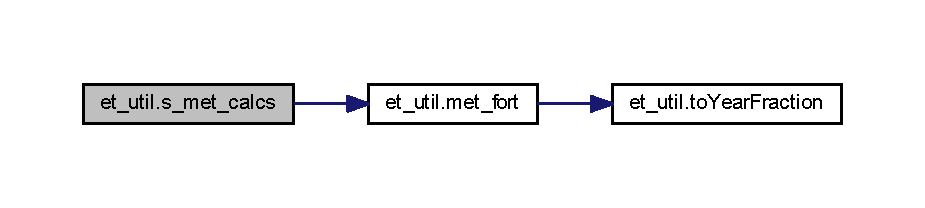
\includegraphics[width=350pt]{namespaceet__util_a28b3adad3d77922fccf7a1d77dd3adda_cgraph}
\end{center}
\end{figure}


\hypertarget{namespaceet__util_a38dc0fbf4d56c116d7f8eb34a893abad}{}\index{et\+\_\+util@{et\+\_\+util}!select\+\_\+dates@{select\+\_\+dates}}
\index{select\+\_\+dates@{select\+\_\+dates}!et\+\_\+util@{et\+\_\+util}}
\subsubsection[{select\+\_\+dates}]{\setlength{\rightskip}{0pt plus 5cm}def et\+\_\+util.\+select\+\_\+dates (
\begin{DoxyParamCaption}
\item[{}]{analysis\+\_\+start, }
\item[{}]{release\+\_\+end, }
\item[{}]{df\+\_\+met, }
\item[{}]{df\+\_\+rad, }
\item[{}]{df\+\_\+ec, }
\item[{}]{df\+\_\+ec\+\_\+all}
\end{DoxyParamCaption}
)}\label{namespaceet__util_a38dc0fbf4d56c116d7f8eb34a893abad}


Definition at line 957 of file et\+\_\+util.\+py.



Here is the caller graph for this function\+:
\nopagebreak
\begin{figure}[H]
\begin{center}
\leavevmode
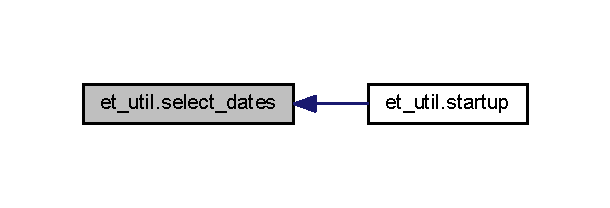
\includegraphics[width=293pt]{namespaceet__util_a38dc0fbf4d56c116d7f8eb34a893abad_icgraph}
\end{center}
\end{figure}


\hypertarget{namespaceet__util_a164b6705ccf94cb947d6bd11c7c19021}{}\index{et\+\_\+util@{et\+\_\+util}!startup@{startup}}
\index{startup@{startup}!et\+\_\+util@{et\+\_\+util}}
\subsubsection[{startup}]{\setlength{\rightskip}{0pt plus 5cm}def et\+\_\+util.\+startup (
\begin{DoxyParamCaption}
\item[{}]{path\+\_\+in, }
\item[{}]{path\+\_\+out, }
\item[{}]{path\+\_\+temp, }
\item[{}]{station, }
\item[{}]{station\+\_\+prefix, }
\item[{}]{analysis\+\_\+start, }
\item[{}]{release\+\_\+start, }
\item[{}]{release\+\_\+end, }
\item[{}]{rebuild, }
\item[{}]{combined\+\_\+echo, }
\item[{}]{echo\+\_\+get}
\end{DoxyParamCaption}
)}\label{namespaceet__util_a164b6705ccf94cb947d6bd11c7c19021}
\begin{DoxyVerb}Checks file status, rebuilds inventory and archive if requested, working files if needed.

:param path_in: Path to raw data files
:param path_out: Path to store processed data
:param path_temp:
:param station: Currently, 's' or 'd'
:param station_prefix: File name prefix for station files
:param analysis_start: Sometimes earlier that release start to support moving averages.
:param release_start: Datetime for start of data report
:param release_end: Datetime for end of data report
:param rebuild: Text request for archive rebuild
:param combined_echo: Logical request for dataframe description of final data to console
:param echo_get:  Logical request for dataframe description of each input file to console
:return: df_ec, df_ec_all, df_met, df_rad
\end{DoxyVerb}
 

Definition at line 39 of file et\+\_\+util.\+py.



Here is the call graph for this function\+:
\nopagebreak
\begin{figure}[H]
\begin{center}
\leavevmode
\includegraphics[width=350pt]{namespaceet__util_a164b6705ccf94cb947d6bd11c7c19021_cgraph}
\end{center}
\end{figure}


\hypertarget{namespaceet__util_a8f87bce6dab1c42c9130fae0df312416}{}\index{et\+\_\+util@{et\+\_\+util}!to\+Year\+Fraction@{to\+Year\+Fraction}}
\index{to\+Year\+Fraction@{to\+Year\+Fraction}!et\+\_\+util@{et\+\_\+util}}
\subsubsection[{to\+Year\+Fraction}]{\setlength{\rightskip}{0pt plus 5cm}def et\+\_\+util.\+to\+Year\+Fraction (
\begin{DoxyParamCaption}
\item[{}]{date}
\end{DoxyParamCaption}
)}\label{namespaceet__util_a8f87bce6dab1c42c9130fae0df312416}
\begin{DoxyVerb}Get decimal year from a scalar python datetime variable.

:param date: datetime variable
:return: date as year fraction

http://stackoverflow.com/questions/6451655/python-how-to-convert-datetime-dates-to-decimal-years
Dependant: write_met_fort()
External Dependencies: datetime, time
\end{DoxyVerb}
 

Definition at line 1751 of file et\+\_\+util.\+py.



Here is the caller graph for this function\+:\nopagebreak
\begin{figure}[H]
\begin{center}
\leavevmode
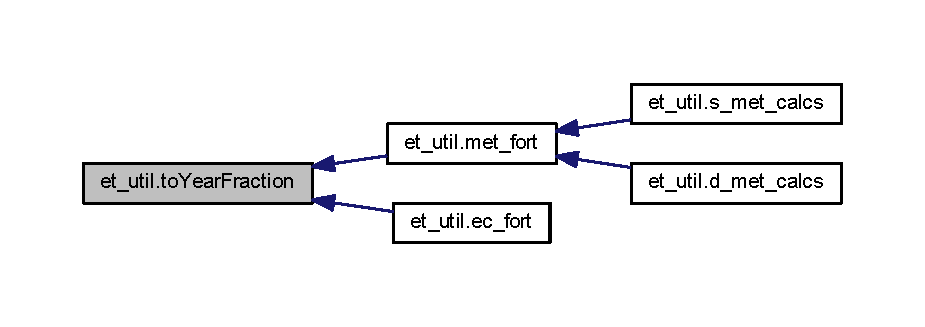
\includegraphics[width=350pt]{namespaceet__util_a8f87bce6dab1c42c9130fae0df312416_icgraph}
\end{center}
\end{figure}


\hypertarget{namespaceet__util_aa4a0538c05ece93097940be5a2ef4204}{}\index{et\+\_\+util@{et\+\_\+util}!write\+\_\+file\+\_\+times@{write\+\_\+file\+\_\+times}}
\index{write\+\_\+file\+\_\+times@{write\+\_\+file\+\_\+times}!et\+\_\+util@{et\+\_\+util}}
\subsubsection[{write\+\_\+file\+\_\+times}]{\setlength{\rightskip}{0pt plus 5cm}def et\+\_\+util.\+write\+\_\+file\+\_\+times (
\begin{DoxyParamCaption}
\item[{}]{config, }
\item[{}]{release\+\_\+start, }
\item[{}]{release\+\_\+end}
\end{DoxyParamCaption}
)}\label{namespaceet__util_aa4a0538c05ece93097940be5a2ef4204}
\begin{DoxyVerb}Writes archive start and end times to Configuration.txt.

:param release_start: start datetime of last archive build
:param release_end: end datetime of last archive build
:return: file_times list

Dependents: main
External Dependencies: datetime
\end{DoxyVerb}
 

Definition at line 189 of file et\+\_\+util.\+py.



Here is the caller graph for this function\+:
\nopagebreak
\begin{figure}[H]
\begin{center}
\leavevmode
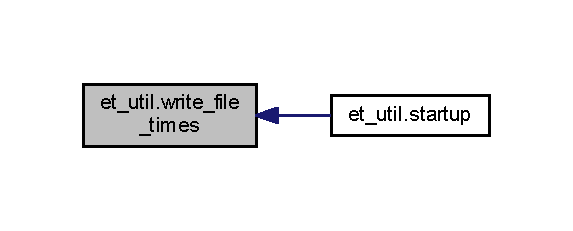
\includegraphics[width=275pt]{namespaceet__util_aa4a0538c05ece93097940be5a2ef4204_icgraph}
\end{center}
\end{figure}


\hypertarget{namespaceet__util_a41b39b3c70ba9961221c284cc738122e}{}\index{et\+\_\+util@{et\+\_\+util}!write\+\_\+raw@{write\+\_\+raw}}
\index{write\+\_\+raw@{write\+\_\+raw}!et\+\_\+util@{et\+\_\+util}}
\subsubsection[{write\+\_\+raw}]{\setlength{\rightskip}{0pt plus 5cm}def et\+\_\+util.\+write\+\_\+raw (
\begin{DoxyParamCaption}
\item[{}]{path\+\_\+out, }
\item[{}]{df\+\_\+met, }
\item[{}]{df\+\_\+rad, }
\item[{}]{df\+\_\+ec, }
\item[{}]{df\+\_\+ec\+\_\+all}
\end{DoxyParamCaption}
)}\label{namespaceet__util_a41b39b3c70ba9961221c284cc738122e}


Definition at line 512 of file et\+\_\+util.\+py.



Here is the caller graph for this function\+:
\nopagebreak
\begin{figure}[H]
\begin{center}
\leavevmode
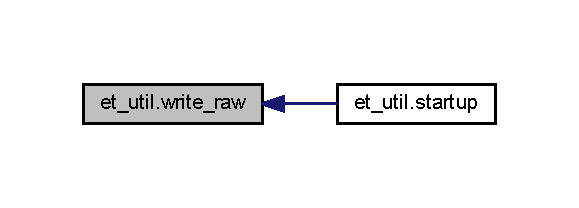
\includegraphics[width=278pt]{namespaceet__util_a41b39b3c70ba9961221c284cc738122e_icgraph}
\end{center}
\end{figure}



\hypertarget{namespace_flag_analysis}{}\section{Flag\+Analysis Namespace Reference}
\label{namespace_flag_analysis}\index{Flag\+Analysis@{Flag\+Analysis}}
\subsection*{Functions}
\begin{DoxyCompactItemize}
\item 
def \hyperlink{namespace_flag_analysis_a4ef4afc0d129e509db5b4e87e7f89520}{get\+\_\+colors} (num\+\_\+colors)
\item 
def \hyperlink{namespace_flag_analysis_aea67ad62c26ead387c02331695c812a1}{get\+\_\+df\+\_\+from\+\_\+file} (path\+\_\+name)
\item 
def \hyperlink{namespace_flag_analysis_a4b1d5d88a8955d1fdb0302a7c316c15c}{refactor\+\_\+time} (\hyperlink{namespace_flag_analysis_ae8822b0eb9daec5247dbcf50515f9809}{df})
\item 
def \hyperlink{namespace_flag_analysis_a3dd518fd2de056580053831b7cc0461c}{save\+\_\+to\+\_\+csv} (\hyperlink{namespace_flag_analysis_ae8822b0eb9daec5247dbcf50515f9809}{df}, path\+\_\+name)
\item 
def \hyperlink{namespace_flag_analysis_a9032e3f92b63876c3a38cc8f6a5e0d3f}{make\+\_\+plot} (\hyperlink{namespace_flag_analysis_a71e45af7a483a1647c8609f98d8b959e}{df\+\_\+pivt}, \hyperlink{namespace_flag_analysis_a2580a0126198e57e3b911e2e9005ce1e}{number\+\_\+of\+\_\+plot\+\_\+colors}, \hyperlink{namespace_flag_analysis_abd038dc9d4b0dae57d6f4ba4218b8f3a}{plot\+\_\+title})
\end{DoxyCompactItemize}
\subsection*{Variables}
\begin{DoxyCompactItemize}
\item 
string \hyperlink{namespace_flag_analysis_a7b5b76152f5c421daf3fbdae1ee42ec5}{\+\_\+\+\_\+author\+\_\+\+\_\+} = \textquotesingle{}mturtora\textquotesingle{}
\item 
string \hyperlink{namespace_flag_analysis_a479e7d01bc47b2c854b2f33d7d8b2719}{path} = \textquotesingle{}..\textbackslash{}\textbackslash{}..\textbackslash{}\textbackslash{}Starkey\textbackslash{}\textbackslash{}process\textbackslash{}\textbackslash{}201505\textbackslash{}\textbackslash{}\textquotesingle{}
\item 
int \hyperlink{namespace_flag_analysis_a2580a0126198e57e3b911e2e9005ce1e}{number\+\_\+of\+\_\+plot\+\_\+colors} = 120
\item 
string \hyperlink{namespace_flag_analysis_a39d797833bc2634e7f4c497cf090bc66}{pivot\+\_\+column\+\_\+name} = \textquotesingle{}Measure\+Flag\textquotesingle{}
\item 
string \hyperlink{namespace_flag_analysis_abd038dc9d4b0dae57d6f4ba4218b8f3a}{plot\+\_\+title} = \textquotesingle{} \textquotesingle{}
\item 
tuple \hyperlink{namespace_flag_analysis_ae8822b0eb9daec5247dbcf50515f9809}{df} = \hyperlink{namespace_flag_analysis_aea67ad62c26ead387c02331695c812a1}{get\+\_\+df\+\_\+from\+\_\+file}(\hyperlink{namespace_flag_analysis_a479e7d01bc47b2c854b2f33d7d8b2719}{path} + \textquotesingle{}Flag\+Analysis.\+csv\textquotesingle{})
\item 
tuple \hyperlink{namespace_flag_analysis_ae886d6e98de0bb5bb5a83e12ed72b924}{df\+\_\+piv} = df.\+pivot(index=\textquotesingle{}date\textquotesingle{}, columns=\textquotesingle{}hm\textquotesingle{}, values=\hyperlink{namespace_flag_analysis_a39d797833bc2634e7f4c497cf090bc66}{pivot\+\_\+column\+\_\+name})
\item 
\hyperlink{namespace_flag_analysis_a71e45af7a483a1647c8609f98d8b959e}{df\+\_\+pivt} = df\+\_\+piv.\+T
\end{DoxyCompactItemize}


\subsection{Function Documentation}
\hypertarget{namespace_flag_analysis_a4ef4afc0d129e509db5b4e87e7f89520}{}\index{Flag\+Analysis@{Flag\+Analysis}!get\+\_\+colors@{get\+\_\+colors}}
\index{get\+\_\+colors@{get\+\_\+colors}!Flag\+Analysis@{Flag\+Analysis}}
\subsubsection[{get\+\_\+colors}]{\setlength{\rightskip}{0pt plus 5cm}def Flag\+Analysis.\+get\+\_\+colors (
\begin{DoxyParamCaption}
\item[{}]{num\+\_\+colors}
\end{DoxyParamCaption}
)}\label{namespace_flag_analysis_a4ef4afc0d129e509db5b4e87e7f89520}


Definition at line 3 of file Flag\+Analysis.\+py.



Here is the caller graph for this function\+:\nopagebreak
\begin{figure}[H]
\begin{center}
\leavevmode
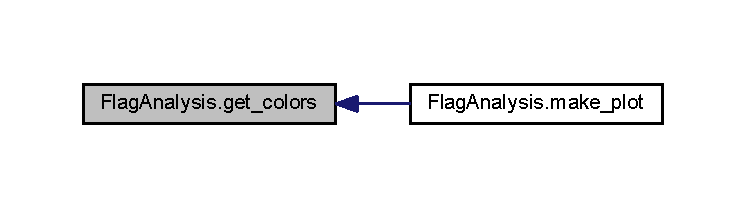
\includegraphics[width=350pt]{namespace_flag_analysis_a4ef4afc0d129e509db5b4e87e7f89520_icgraph}
\end{center}
\end{figure}


\hypertarget{namespace_flag_analysis_aea67ad62c26ead387c02331695c812a1}{}\index{Flag\+Analysis@{Flag\+Analysis}!get\+\_\+df\+\_\+from\+\_\+file@{get\+\_\+df\+\_\+from\+\_\+file}}
\index{get\+\_\+df\+\_\+from\+\_\+file@{get\+\_\+df\+\_\+from\+\_\+file}!Flag\+Analysis@{Flag\+Analysis}}
\subsubsection[{get\+\_\+df\+\_\+from\+\_\+file}]{\setlength{\rightskip}{0pt plus 5cm}def Flag\+Analysis.\+get\+\_\+df\+\_\+from\+\_\+file (
\begin{DoxyParamCaption}
\item[{}]{path\+\_\+name}
\end{DoxyParamCaption}
)}\label{namespace_flag_analysis_aea67ad62c26ead387c02331695c812a1}


Definition at line 15 of file Flag\+Analysis.\+py.

\hypertarget{namespace_flag_analysis_a9032e3f92b63876c3a38cc8f6a5e0d3f}{}\index{Flag\+Analysis@{Flag\+Analysis}!make\+\_\+plot@{make\+\_\+plot}}
\index{make\+\_\+plot@{make\+\_\+plot}!Flag\+Analysis@{Flag\+Analysis}}
\subsubsection[{make\+\_\+plot}]{\setlength{\rightskip}{0pt plus 5cm}def Flag\+Analysis.\+make\+\_\+plot (
\begin{DoxyParamCaption}
\item[{}]{df\+\_\+pivt, }
\item[{}]{number\+\_\+of\+\_\+plot\+\_\+colors, }
\item[{}]{plot\+\_\+title}
\end{DoxyParamCaption}
)}\label{namespace_flag_analysis_a9032e3f92b63876c3a38cc8f6a5e0d3f}


Definition at line 33 of file Flag\+Analysis.\+py.



Here is the call graph for this function\+:\nopagebreak
\begin{figure}[H]
\begin{center}
\leavevmode
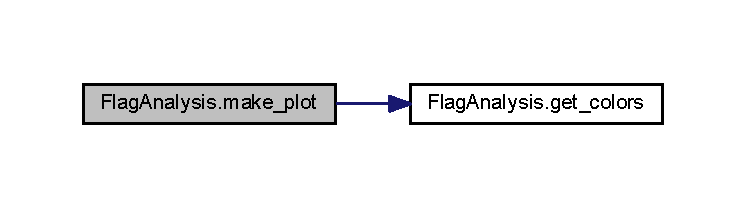
\includegraphics[width=350pt]{namespace_flag_analysis_a9032e3f92b63876c3a38cc8f6a5e0d3f_cgraph}
\end{center}
\end{figure}


\hypertarget{namespace_flag_analysis_a4b1d5d88a8955d1fdb0302a7c316c15c}{}\index{Flag\+Analysis@{Flag\+Analysis}!refactor\+\_\+time@{refactor\+\_\+time}}
\index{refactor\+\_\+time@{refactor\+\_\+time}!Flag\+Analysis@{Flag\+Analysis}}
\subsubsection[{refactor\+\_\+time}]{\setlength{\rightskip}{0pt plus 5cm}def Flag\+Analysis.\+refactor\+\_\+time (
\begin{DoxyParamCaption}
\item[{}]{df}
\end{DoxyParamCaption}
)}\label{namespace_flag_analysis_a4b1d5d88a8955d1fdb0302a7c316c15c}


Definition at line 19 of file Flag\+Analysis.\+py.

\hypertarget{namespace_flag_analysis_a3dd518fd2de056580053831b7cc0461c}{}\index{Flag\+Analysis@{Flag\+Analysis}!save\+\_\+to\+\_\+csv@{save\+\_\+to\+\_\+csv}}
\index{save\+\_\+to\+\_\+csv@{save\+\_\+to\+\_\+csv}!Flag\+Analysis@{Flag\+Analysis}}
\subsubsection[{save\+\_\+to\+\_\+csv}]{\setlength{\rightskip}{0pt plus 5cm}def Flag\+Analysis.\+save\+\_\+to\+\_\+csv (
\begin{DoxyParamCaption}
\item[{}]{df, }
\item[{}]{path\+\_\+name}
\end{DoxyParamCaption}
)}\label{namespace_flag_analysis_a3dd518fd2de056580053831b7cc0461c}


Definition at line 28 of file Flag\+Analysis.\+py.



\subsection{Variable Documentation}
\hypertarget{namespace_flag_analysis_a7b5b76152f5c421daf3fbdae1ee42ec5}{}\index{Flag\+Analysis@{Flag\+Analysis}!\+\_\+\+\_\+author\+\_\+\+\_\+@{\+\_\+\+\_\+author\+\_\+\+\_\+}}
\index{\+\_\+\+\_\+author\+\_\+\+\_\+@{\+\_\+\+\_\+author\+\_\+\+\_\+}!Flag\+Analysis@{Flag\+Analysis}}
\subsubsection[{\+\_\+\+\_\+author\+\_\+\+\_\+}]{\setlength{\rightskip}{0pt plus 5cm}string Flag\+Analysis.\+\_\+\+\_\+author\+\_\+\+\_\+ = \textquotesingle{}mturtora\textquotesingle{}}\label{namespace_flag_analysis_a7b5b76152f5c421daf3fbdae1ee42ec5}


Definition at line 45 of file Flag\+Analysis.\+py.

\hypertarget{namespace_flag_analysis_ae8822b0eb9daec5247dbcf50515f9809}{}\index{Flag\+Analysis@{Flag\+Analysis}!df@{df}}
\index{df@{df}!Flag\+Analysis@{Flag\+Analysis}}
\subsubsection[{df}]{\setlength{\rightskip}{0pt plus 5cm}tuple Flag\+Analysis.\+df = {\bf get\+\_\+df\+\_\+from\+\_\+file}({\bf path} + \textquotesingle{}Flag\+Analysis.\+csv\textquotesingle{})}\label{namespace_flag_analysis_ae8822b0eb9daec5247dbcf50515f9809}


Definition at line 69 of file Flag\+Analysis.\+py.

\hypertarget{namespace_flag_analysis_ae886d6e98de0bb5bb5a83e12ed72b924}{}\index{Flag\+Analysis@{Flag\+Analysis}!df\+\_\+piv@{df\+\_\+piv}}
\index{df\+\_\+piv@{df\+\_\+piv}!Flag\+Analysis@{Flag\+Analysis}}
\subsubsection[{df\+\_\+piv}]{\setlength{\rightskip}{0pt plus 5cm}tuple Flag\+Analysis.\+df\+\_\+piv = df.\+pivot(index=\textquotesingle{}date\textquotesingle{}, columns=\textquotesingle{}hm\textquotesingle{}, values={\bf pivot\+\_\+column\+\_\+name})}\label{namespace_flag_analysis_ae886d6e98de0bb5bb5a83e12ed72b924}


Definition at line 76 of file Flag\+Analysis.\+py.

\hypertarget{namespace_flag_analysis_a71e45af7a483a1647c8609f98d8b959e}{}\index{Flag\+Analysis@{Flag\+Analysis}!df\+\_\+pivt@{df\+\_\+pivt}}
\index{df\+\_\+pivt@{df\+\_\+pivt}!Flag\+Analysis@{Flag\+Analysis}}
\subsubsection[{df\+\_\+pivt}]{\setlength{\rightskip}{0pt plus 5cm}Flag\+Analysis.\+df\+\_\+pivt = df\+\_\+piv.\+T}\label{namespace_flag_analysis_a71e45af7a483a1647c8609f98d8b959e}


Definition at line 87 of file Flag\+Analysis.\+py.

\hypertarget{namespace_flag_analysis_a2580a0126198e57e3b911e2e9005ce1e}{}\index{Flag\+Analysis@{Flag\+Analysis}!number\+\_\+of\+\_\+plot\+\_\+colors@{number\+\_\+of\+\_\+plot\+\_\+colors}}
\index{number\+\_\+of\+\_\+plot\+\_\+colors@{number\+\_\+of\+\_\+plot\+\_\+colors}!Flag\+Analysis@{Flag\+Analysis}}
\subsubsection[{number\+\_\+of\+\_\+plot\+\_\+colors}]{\setlength{\rightskip}{0pt plus 5cm}int Flag\+Analysis.\+number\+\_\+of\+\_\+plot\+\_\+colors = 120}\label{namespace_flag_analysis_a2580a0126198e57e3b911e2e9005ce1e}


Definition at line 64 of file Flag\+Analysis.\+py.

\hypertarget{namespace_flag_analysis_a479e7d01bc47b2c854b2f33d7d8b2719}{}\index{Flag\+Analysis@{Flag\+Analysis}!path@{path}}
\index{path@{path}!Flag\+Analysis@{Flag\+Analysis}}
\subsubsection[{path}]{\setlength{\rightskip}{0pt plus 5cm}string Flag\+Analysis.\+path = \textquotesingle{}..\textbackslash{}\textbackslash{}..\textbackslash{}\textbackslash{}Starkey\textbackslash{}\textbackslash{}process\textbackslash{}\textbackslash{}201505\textbackslash{}\textbackslash{}\textquotesingle{}}\label{namespace_flag_analysis_a479e7d01bc47b2c854b2f33d7d8b2719}


Definition at line 50 of file Flag\+Analysis.\+py.

\hypertarget{namespace_flag_analysis_a39d797833bc2634e7f4c497cf090bc66}{}\index{Flag\+Analysis@{Flag\+Analysis}!pivot\+\_\+column\+\_\+name@{pivot\+\_\+column\+\_\+name}}
\index{pivot\+\_\+column\+\_\+name@{pivot\+\_\+column\+\_\+name}!Flag\+Analysis@{Flag\+Analysis}}
\subsubsection[{pivot\+\_\+column\+\_\+name}]{\setlength{\rightskip}{0pt plus 5cm}string Flag\+Analysis.\+pivot\+\_\+column\+\_\+name = \textquotesingle{}Measure\+Flag\textquotesingle{}}\label{namespace_flag_analysis_a39d797833bc2634e7f4c497cf090bc66}


Definition at line 65 of file Flag\+Analysis.\+py.

\hypertarget{namespace_flag_analysis_abd038dc9d4b0dae57d6f4ba4218b8f3a}{}\index{Flag\+Analysis@{Flag\+Analysis}!plot\+\_\+title@{plot\+\_\+title}}
\index{plot\+\_\+title@{plot\+\_\+title}!Flag\+Analysis@{Flag\+Analysis}}
\subsubsection[{plot\+\_\+title}]{\setlength{\rightskip}{0pt plus 5cm}string Flag\+Analysis.\+plot\+\_\+title = \textquotesingle{} \textquotesingle{}}\label{namespace_flag_analysis_abd038dc9d4b0dae57d6f4ba4218b8f3a}


Definition at line 67 of file Flag\+Analysis.\+py.


\hypertarget{namespacegap_tests}{}\section{gap\+Tests Namespace Reference}
\label{namespacegap_tests}\index{gap\+Tests@{gap\+Tests}}
\subsection*{Variables}
\begin{DoxyCompactItemize}
\item 
string \hyperlink{namespacegap_tests_a7601773bbec9b1e705d8dcacec0cecd4}{\+\_\+\+\_\+author\+\_\+\+\_\+} = \textquotesingle{}mturtora\textquotesingle{}
\item 
string \hyperlink{namespacegap_tests_a3f57b56fc8e69d0dcd827c75f6743077}{path} = \textquotesingle{}datastore\textbackslash{}\textbackslash{}\+Dead\+River\+\_\+01\textbackslash{}\textbackslash{}\textquotesingle{}
\item 
tuple \hyperlink{namespacegap_tests_ad25db032c69bfc31e323da6fb64c808d}{df\+\_\+gaps} = pd.\+read\+\_\+csv(\hyperlink{namespacegap_tests_a3f57b56fc8e69d0dcd827c75f6743077}{path} + \textquotesingle{}gap\+\_\+met.\+csv\textquotesingle{}, index\+\_\+col=\textquotesingle{}Index\textquotesingle{})
\item 
\hyperlink{namespacegap_tests_aea36505be1591db057e57303d8fe98cf}{looped} = False
\item 
tuple \hyperlink{namespacegap_tests_aaf8a186769b9c7f206ec21bc0c710dfc}{gap\+\_\+date\+\_\+index} = pd.\+date\+\_\+range(index, periods=value, freq=\textquotesingle{}30min\textquotesingle{})
\item 
tuple \hyperlink{namespacegap_tests_a350ecaddda824acaaadc5c9162516906}{s\+\_\+gap} = pd.\+Series(value, index=\hyperlink{namespacegap_tests_aaf8a186769b9c7f206ec21bc0c710dfc}{gap\+\_\+date\+\_\+index})
\item 
\hyperlink{namespacegap_tests_ab33889c225b00a0897051f8b89d74acd}{s\+\_\+mask} = \hyperlink{namespacegap_tests_a350ecaddda824acaaadc5c9162516906}{s\+\_\+gap}
\end{DoxyCompactItemize}


\subsection{Variable Documentation}
\hypertarget{namespacegap_tests_a7601773bbec9b1e705d8dcacec0cecd4}{}\index{gap\+Tests@{gap\+Tests}!\+\_\+\+\_\+author\+\_\+\+\_\+@{\+\_\+\+\_\+author\+\_\+\+\_\+}}
\index{\+\_\+\+\_\+author\+\_\+\+\_\+@{\+\_\+\+\_\+author\+\_\+\+\_\+}!gap\+Tests@{gap\+Tests}}
\subsubsection[{\+\_\+\+\_\+author\+\_\+\+\_\+}]{\setlength{\rightskip}{0pt plus 5cm}string gap\+Tests.\+\_\+\+\_\+author\+\_\+\+\_\+ = \textquotesingle{}mturtora\textquotesingle{}}\label{namespacegap_tests_a7601773bbec9b1e705d8dcacec0cecd4}


Definition at line 6 of file gap\+Tests.\+py.

\hypertarget{namespacegap_tests_ad25db032c69bfc31e323da6fb64c808d}{}\index{gap\+Tests@{gap\+Tests}!df\+\_\+gaps@{df\+\_\+gaps}}
\index{df\+\_\+gaps@{df\+\_\+gaps}!gap\+Tests@{gap\+Tests}}
\subsubsection[{df\+\_\+gaps}]{\setlength{\rightskip}{0pt plus 5cm}list gap\+Tests.\+df\+\_\+gaps = pd.\+read\+\_\+csv({\bf path} + \textquotesingle{}gap\+\_\+met.\+csv\textquotesingle{}, index\+\_\+col=\textquotesingle{}Index\textquotesingle{})}\label{namespacegap_tests_ad25db032c69bfc31e323da6fb64c808d}


Definition at line 12 of file gap\+Tests.\+py.

\hypertarget{namespacegap_tests_aaf8a186769b9c7f206ec21bc0c710dfc}{}\index{gap\+Tests@{gap\+Tests}!gap\+\_\+date\+\_\+index@{gap\+\_\+date\+\_\+index}}
\index{gap\+\_\+date\+\_\+index@{gap\+\_\+date\+\_\+index}!gap\+Tests@{gap\+Tests}}
\subsubsection[{gap\+\_\+date\+\_\+index}]{\setlength{\rightskip}{0pt plus 5cm}tuple gap\+Tests.\+gap\+\_\+date\+\_\+index = pd.\+date\+\_\+range(index, periods=value, freq=\textquotesingle{}30min\textquotesingle{})}\label{namespacegap_tests_aaf8a186769b9c7f206ec21bc0c710dfc}


Definition at line 20 of file gap\+Tests.\+py.

\hypertarget{namespacegap_tests_aea36505be1591db057e57303d8fe98cf}{}\index{gap\+Tests@{gap\+Tests}!looped@{looped}}
\index{looped@{looped}!gap\+Tests@{gap\+Tests}}
\subsubsection[{looped}]{\setlength{\rightskip}{0pt plus 5cm}gap\+Tests.\+looped = False}\label{namespacegap_tests_aea36505be1591db057e57303d8fe98cf}


Definition at line 16 of file gap\+Tests.\+py.

\hypertarget{namespacegap_tests_a3f57b56fc8e69d0dcd827c75f6743077}{}\index{gap\+Tests@{gap\+Tests}!path@{path}}
\index{path@{path}!gap\+Tests@{gap\+Tests}}
\subsubsection[{path}]{\setlength{\rightskip}{0pt plus 5cm}string gap\+Tests.\+path = \textquotesingle{}datastore\textbackslash{}\textbackslash{}\+Dead\+River\+\_\+01\textbackslash{}\textbackslash{}\textquotesingle{}}\label{namespacegap_tests_a3f57b56fc8e69d0dcd827c75f6743077}


Definition at line 11 of file gap\+Tests.\+py.

\hypertarget{namespacegap_tests_a350ecaddda824acaaadc5c9162516906}{}\index{gap\+Tests@{gap\+Tests}!s\+\_\+gap@{s\+\_\+gap}}
\index{s\+\_\+gap@{s\+\_\+gap}!gap\+Tests@{gap\+Tests}}
\subsubsection[{s\+\_\+gap}]{\setlength{\rightskip}{0pt plus 5cm}tuple gap\+Tests.\+s\+\_\+gap = pd.\+Series(value, index={\bf gap\+\_\+date\+\_\+index})}\label{namespacegap_tests_a350ecaddda824acaaadc5c9162516906}


Definition at line 21 of file gap\+Tests.\+py.

\hypertarget{namespacegap_tests_ab33889c225b00a0897051f8b89d74acd}{}\index{gap\+Tests@{gap\+Tests}!s\+\_\+mask@{s\+\_\+mask}}
\index{s\+\_\+mask@{s\+\_\+mask}!gap\+Tests@{gap\+Tests}}
\subsubsection[{s\+\_\+mask}]{\setlength{\rightskip}{0pt plus 5cm}tuple gap\+Tests.\+s\+\_\+mask = {\bf s\+\_\+gap}}\label{namespacegap_tests_ab33889c225b00a0897051f8b89d74acd}


Definition at line 25 of file gap\+Tests.\+py.


\hypertarget{namespaceheatmap__slopes}{}\section{heatmap\+\_\+slopes Namespace Reference}
\label{namespaceheatmap__slopes}\index{heatmap\+\_\+slopes@{heatmap\+\_\+slopes}}
\subsection*{Functions}
\begin{DoxyCompactItemize}
\item 
def \hyperlink{namespaceheatmap__slopes_a33c45e5d0e9e92c296e18f8ca66b5638}{read\+\_\+file} (\hyperlink{namespaceheatmap__slopes_ad5603c14f73e42c82621c93fe6d44b26}{path})
\end{DoxyCompactItemize}
\subsection*{Variables}
\begin{DoxyCompactItemize}
\item 
string \hyperlink{namespaceheatmap__slopes_ab7a46011bf1690c1bbf4d0d9b90ff55a}{\+\_\+\+\_\+author\+\_\+\+\_\+} = \textquotesingle{}mturtora\textquotesingle{}
\item 
string \hyperlink{namespaceheatmap__slopes_ad5603c14f73e42c82621c93fe6d44b26}{path} = \textquotesingle{}I\+:\textbackslash{}\textbackslash{}\+A\+L\+L\textbackslash{}\textbackslash{}\+Tampa\+E\+T\textbackslash{}\textbackslash{}\+Starkey\textbackslash{}\textbackslash{}process\textbackslash{}\textbackslash{}201505\textbackslash{}\textbackslash{}\textquotesingle{}
\item 
tuple \hyperlink{namespaceheatmap__slopes_ac3ee4dd583b7c5cd73fbdc02298c4dcb}{df} = \hyperlink{namespaceheatmap__slopes_a33c45e5d0e9e92c296e18f8ca66b5638}{read\+\_\+file}(\hyperlink{namespaceheatmap__slopes_ad5603c14f73e42c82621c93fe6d44b26}{path} + \textquotesingle{}slopes.\+csv\textquotesingle{})
\item 
\hyperlink{namespaceheatmap__slopes_aa1c2bb69edf12eba2a35308bd4d5fc54}{x} = df.\+Begin.\+values
\item 
\hyperlink{namespaceheatmap__slopes_afe0805836a2ce30217aa9093142eee6e}{y} = df.\+Slope.\+values
\item 
\hyperlink{namespaceheatmap__slopes_abe09eedeaabe04604f446a88d9999f20}{custom\+\_\+colors} = df.\+End.\+values
\end{DoxyCompactItemize}


\subsection{Function Documentation}
\hypertarget{namespaceheatmap__slopes_a33c45e5d0e9e92c296e18f8ca66b5638}{}\index{heatmap\+\_\+slopes@{heatmap\+\_\+slopes}!read\+\_\+file@{read\+\_\+file}}
\index{read\+\_\+file@{read\+\_\+file}!heatmap\+\_\+slopes@{heatmap\+\_\+slopes}}
\subsubsection[{read\+\_\+file}]{\setlength{\rightskip}{0pt plus 5cm}def heatmap\+\_\+slopes.\+read\+\_\+file (
\begin{DoxyParamCaption}
\item[{}]{path}
\end{DoxyParamCaption}
)}\label{namespaceheatmap__slopes_a33c45e5d0e9e92c296e18f8ca66b5638}


Definition at line 9 of file heatmap\+\_\+slopes.\+py.



\subsection{Variable Documentation}
\hypertarget{namespaceheatmap__slopes_ab7a46011bf1690c1bbf4d0d9b90ff55a}{}\index{heatmap\+\_\+slopes@{heatmap\+\_\+slopes}!\+\_\+\+\_\+author\+\_\+\+\_\+@{\+\_\+\+\_\+author\+\_\+\+\_\+}}
\index{\+\_\+\+\_\+author\+\_\+\+\_\+@{\+\_\+\+\_\+author\+\_\+\+\_\+}!heatmap\+\_\+slopes@{heatmap\+\_\+slopes}}
\subsubsection[{\+\_\+\+\_\+author\+\_\+\+\_\+}]{\setlength{\rightskip}{0pt plus 5cm}string heatmap\+\_\+slopes.\+\_\+\+\_\+author\+\_\+\+\_\+ = \textquotesingle{}mturtora\textquotesingle{}}\label{namespaceheatmap__slopes_ab7a46011bf1690c1bbf4d0d9b90ff55a}


Definition at line 1 of file heatmap\+\_\+slopes.\+py.

\hypertarget{namespaceheatmap__slopes_abe09eedeaabe04604f446a88d9999f20}{}\index{heatmap\+\_\+slopes@{heatmap\+\_\+slopes}!custom\+\_\+colors@{custom\+\_\+colors}}
\index{custom\+\_\+colors@{custom\+\_\+colors}!heatmap\+\_\+slopes@{heatmap\+\_\+slopes}}
\subsubsection[{custom\+\_\+colors}]{\setlength{\rightskip}{0pt plus 5cm}heatmap\+\_\+slopes.\+custom\+\_\+colors = df.\+End.\+values}\label{namespaceheatmap__slopes_abe09eedeaabe04604f446a88d9999f20}


Definition at line 23 of file heatmap\+\_\+slopes.\+py.

\hypertarget{namespaceheatmap__slopes_ac3ee4dd583b7c5cd73fbdc02298c4dcb}{}\index{heatmap\+\_\+slopes@{heatmap\+\_\+slopes}!df@{df}}
\index{df@{df}!heatmap\+\_\+slopes@{heatmap\+\_\+slopes}}
\subsubsection[{df}]{\setlength{\rightskip}{0pt plus 5cm}list heatmap\+\_\+slopes.\+df = {\bf read\+\_\+file}({\bf path} + \textquotesingle{}slopes.\+csv\textquotesingle{})}\label{namespaceheatmap__slopes_ac3ee4dd583b7c5cd73fbdc02298c4dcb}


Definition at line 16 of file heatmap\+\_\+slopes.\+py.

\hypertarget{namespaceheatmap__slopes_ad5603c14f73e42c82621c93fe6d44b26}{}\index{heatmap\+\_\+slopes@{heatmap\+\_\+slopes}!path@{path}}
\index{path@{path}!heatmap\+\_\+slopes@{heatmap\+\_\+slopes}}
\subsubsection[{path}]{\setlength{\rightskip}{0pt plus 5cm}string heatmap\+\_\+slopes.\+path = \textquotesingle{}I\+:\textbackslash{}\textbackslash{}\+A\+L\+L\textbackslash{}\textbackslash{}\+Tampa\+E\+T\textbackslash{}\textbackslash{}\+Starkey\textbackslash{}\textbackslash{}process\textbackslash{}\textbackslash{}201505\textbackslash{}\textbackslash{}\textquotesingle{}}\label{namespaceheatmap__slopes_ad5603c14f73e42c82621c93fe6d44b26}


Definition at line 15 of file heatmap\+\_\+slopes.\+py.

\hypertarget{namespaceheatmap__slopes_aa1c2bb69edf12eba2a35308bd4d5fc54}{}\index{heatmap\+\_\+slopes@{heatmap\+\_\+slopes}!x@{x}}
\index{x@{x}!heatmap\+\_\+slopes@{heatmap\+\_\+slopes}}
\subsubsection[{x}]{\setlength{\rightskip}{0pt plus 5cm}heatmap\+\_\+slopes.\+x = df.\+Begin.\+values}\label{namespaceheatmap__slopes_aa1c2bb69edf12eba2a35308bd4d5fc54}


Definition at line 21 of file heatmap\+\_\+slopes.\+py.

\hypertarget{namespaceheatmap__slopes_afe0805836a2ce30217aa9093142eee6e}{}\index{heatmap\+\_\+slopes@{heatmap\+\_\+slopes}!y@{y}}
\index{y@{y}!heatmap\+\_\+slopes@{heatmap\+\_\+slopes}}
\subsubsection[{y}]{\setlength{\rightskip}{0pt plus 5cm}heatmap\+\_\+slopes.\+y = df.\+Slope.\+values}\label{namespaceheatmap__slopes_afe0805836a2ce30217aa9093142eee6e}


Definition at line 22 of file heatmap\+\_\+slopes.\+py.


\hypertarget{namespaceheatmap__subplots}{}\section{heatmap\+\_\+subplots Namespace Reference}
\label{namespaceheatmap__subplots}\index{heatmap\+\_\+subplots@{heatmap\+\_\+subplots}}
\subsection*{Functions}
\begin{DoxyCompactItemize}
\item 
def \hyperlink{namespaceheatmap__subplots_ad7968080746de03ee0c2965d50fe0ebd}{read\+\_\+file} (\hyperlink{namespaceheatmap__subplots_ab7df7a9753e857e63f1f8b0490859a31}{path})
\item 
def \hyperlink{namespaceheatmap__subplots_aa29417a7896e55be0a2a79e1ac33efdc}{get\+\_\+xyc} (\hyperlink{namespaceheatmap__subplots_aefdcfb560a154ac398cf52bf39a33cb0}{df})
\end{DoxyCompactItemize}
\subsection*{Variables}
\begin{DoxyCompactItemize}
\item 
string \hyperlink{namespaceheatmap__subplots_a6af073c5f9bb38afeae2782d94abee9e}{\+\_\+\+\_\+author\+\_\+\+\_\+} = \textquotesingle{}mturtora\textquotesingle{}
\item 
string \hyperlink{namespaceheatmap__subplots_ab7df7a9753e857e63f1f8b0490859a31}{path} = \textquotesingle{}I\+:\textbackslash{}\textbackslash{}\+A\+L\+L\textbackslash{}\textbackslash{}\+Tampa\+E\+T\textbackslash{}\textbackslash{}\+Starkey\textbackslash{}\textbackslash{}process\textbackslash{}\textbackslash{}201505\textbackslash{}\textbackslash{}\textquotesingle{}
\item 
tuple \hyperlink{namespaceheatmap__subplots_aefdcfb560a154ac398cf52bf39a33cb0}{df} = \hyperlink{namespaceheatmap__subplots_ad7968080746de03ee0c2965d50fe0ebd}{read\+\_\+file}(\hyperlink{namespaceheatmap__subplots_ab7df7a9753e857e63f1f8b0490859a31}{path} + \textquotesingle{}slopes.\+csv\textquotesingle{})
\item 
list \hyperlink{namespaceheatmap__subplots_a38f24e9de53aa8a935925a0154e4b576}{df\+\_\+13} = df.\+ix\mbox{[}df.\+Year == 2013\mbox{]}
\item 
list \hyperlink{namespaceheatmap__subplots_a664795795d2c75a026821e0bd2a32159}{df\+\_\+14} = df.\+ix\mbox{[}df.\+Year == 2014\mbox{]}
\item 
tuple \hyperlink{namespaceheatmap__subplots_af3b54e7f6c49dd1ad4ed6d5cef1541d0}{df\+\_\+piv} = df\+\_\+13.\+pivot(index=\textquotesingle{}End\textquotesingle{}, columns=\textquotesingle{}Begin\textquotesingle{}, values=\textquotesingle{}Slope\textquotesingle{})
\item 
\hyperlink{namespaceheatmap__subplots_ad2fa7e90b3ea750418e7bfe6c549745f}{Z} = df\+\_\+piv.\+values
\item 
list \hyperlink{namespaceheatmap__subplots_adf6fc02d1af5885087dea1400cdcc546}{begin} = \hyperlink{namespaceheatmap__subplots_a38f24e9de53aa8a935925a0154e4b576}{df\+\_\+13}\mbox{[}\textquotesingle{}Begin\textquotesingle{}\mbox{]}
\item 
list \hyperlink{namespaceheatmap__subplots_a8add050a641ed8526f32e354fffdee93}{end} = \hyperlink{namespaceheatmap__subplots_a38f24e9de53aa8a935925a0154e4b576}{df\+\_\+13}\mbox{[}\textquotesingle{}End\textquotesingle{}\mbox{]}
\item 
tuple \hyperlink{namespaceheatmap__subplots_a7c42f3ab7941ef3754f98b938080fbd4}{C\+S}
\item 
\hyperlink{namespaceheatmap__subplots_a65159fa9d4b96b5413a4469f96972503}{cmap} = plt.\+cm.\+Oranges)
\item 
tuple \hyperlink{namespaceheatmap__subplots_a737acb8a319fcdea231ba28a1fde0f07}{cbar} = plt.\+colorbar(\hyperlink{namespaceheatmap__subplots_a7c42f3ab7941ef3754f98b938080fbd4}{C\+S})
\end{DoxyCompactItemize}


\subsection{Function Documentation}
\hypertarget{namespaceheatmap__subplots_aa29417a7896e55be0a2a79e1ac33efdc}{}\index{heatmap\+\_\+subplots@{heatmap\+\_\+subplots}!get\+\_\+xyc@{get\+\_\+xyc}}
\index{get\+\_\+xyc@{get\+\_\+xyc}!heatmap\+\_\+subplots@{heatmap\+\_\+subplots}}
\subsubsection[{get\+\_\+xyc}]{\setlength{\rightskip}{0pt plus 5cm}def heatmap\+\_\+subplots.\+get\+\_\+xyc (
\begin{DoxyParamCaption}
\item[{}]{df}
\end{DoxyParamCaption}
)}\label{namespaceheatmap__subplots_aa29417a7896e55be0a2a79e1ac33efdc}


Definition at line 13 of file heatmap\+\_\+subplots.\+py.

\hypertarget{namespaceheatmap__subplots_ad7968080746de03ee0c2965d50fe0ebd}{}\index{heatmap\+\_\+subplots@{heatmap\+\_\+subplots}!read\+\_\+file@{read\+\_\+file}}
\index{read\+\_\+file@{read\+\_\+file}!heatmap\+\_\+subplots@{heatmap\+\_\+subplots}}
\subsubsection[{read\+\_\+file}]{\setlength{\rightskip}{0pt plus 5cm}def heatmap\+\_\+subplots.\+read\+\_\+file (
\begin{DoxyParamCaption}
\item[{}]{path}
\end{DoxyParamCaption}
)}\label{namespaceheatmap__subplots_ad7968080746de03ee0c2965d50fe0ebd}


Definition at line 9 of file heatmap\+\_\+subplots.\+py.



\subsection{Variable Documentation}
\hypertarget{namespaceheatmap__subplots_a6af073c5f9bb38afeae2782d94abee9e}{}\index{heatmap\+\_\+subplots@{heatmap\+\_\+subplots}!\+\_\+\+\_\+author\+\_\+\+\_\+@{\+\_\+\+\_\+author\+\_\+\+\_\+}}
\index{\+\_\+\+\_\+author\+\_\+\+\_\+@{\+\_\+\+\_\+author\+\_\+\+\_\+}!heatmap\+\_\+subplots@{heatmap\+\_\+subplots}}
\subsubsection[{\+\_\+\+\_\+author\+\_\+\+\_\+}]{\setlength{\rightskip}{0pt plus 5cm}string heatmap\+\_\+subplots.\+\_\+\+\_\+author\+\_\+\+\_\+ = \textquotesingle{}mturtora\textquotesingle{}}\label{namespaceheatmap__subplots_a6af073c5f9bb38afeae2782d94abee9e}


Definition at line 1 of file heatmap\+\_\+subplots.\+py.

\hypertarget{namespaceheatmap__subplots_adf6fc02d1af5885087dea1400cdcc546}{}\index{heatmap\+\_\+subplots@{heatmap\+\_\+subplots}!begin@{begin}}
\index{begin@{begin}!heatmap\+\_\+subplots@{heatmap\+\_\+subplots}}
\subsubsection[{begin}]{\setlength{\rightskip}{0pt plus 5cm}list heatmap\+\_\+subplots.\+begin = {\bf df\+\_\+13}\mbox{[}\textquotesingle{}Begin\textquotesingle{}\mbox{]}}\label{namespaceheatmap__subplots_adf6fc02d1af5885087dea1400cdcc546}


Definition at line 38 of file heatmap\+\_\+subplots.\+py.

\hypertarget{namespaceheatmap__subplots_a737acb8a319fcdea231ba28a1fde0f07}{}\index{heatmap\+\_\+subplots@{heatmap\+\_\+subplots}!cbar@{cbar}}
\index{cbar@{cbar}!heatmap\+\_\+subplots@{heatmap\+\_\+subplots}}
\subsubsection[{cbar}]{\setlength{\rightskip}{0pt plus 5cm}tuple heatmap\+\_\+subplots.\+cbar = plt.\+colorbar({\bf C\+S})}\label{namespaceheatmap__subplots_a737acb8a319fcdea231ba28a1fde0f07}


Definition at line 46 of file heatmap\+\_\+subplots.\+py.

\hypertarget{namespaceheatmap__subplots_a65159fa9d4b96b5413a4469f96972503}{}\index{heatmap\+\_\+subplots@{heatmap\+\_\+subplots}!cmap@{cmap}}
\index{cmap@{cmap}!heatmap\+\_\+subplots@{heatmap\+\_\+subplots}}
\subsubsection[{cmap}]{\setlength{\rightskip}{0pt plus 5cm}heatmap\+\_\+subplots.\+cmap = plt.\+cm.\+Oranges)}\label{namespaceheatmap__subplots_a65159fa9d4b96b5413a4469f96972503}


Definition at line 45 of file heatmap\+\_\+subplots.\+py.

\hypertarget{namespaceheatmap__subplots_a7c42f3ab7941ef3754f98b938080fbd4}{}\index{heatmap\+\_\+subplots@{heatmap\+\_\+subplots}!C\+S@{C\+S}}
\index{C\+S@{C\+S}!heatmap\+\_\+subplots@{heatmap\+\_\+subplots}}
\subsubsection[{C\+S}]{\setlength{\rightskip}{0pt plus 5cm}tuple heatmap\+\_\+subplots.\+C\+S}\label{namespaceheatmap__subplots_a7c42f3ab7941ef3754f98b938080fbd4}
{\bfseries Initial value\+:}
\begin{DoxyCode}
1 = plt.imshow(Z, aspect=\textcolor{stringliteral}{'auto'}, interpolation=\textcolor{stringliteral}{'none'}, origin=\textcolor{stringliteral}{'lower'},
2                     extent=(Xi.min(), Xi.max(), Yi.min(), Yi.max()),
3                     \textcolor{comment}{#cmap=plt.cm.Blues)}
\end{DoxyCode}


Definition at line 41 of file heatmap\+\_\+subplots.\+py.

\hypertarget{namespaceheatmap__subplots_aefdcfb560a154ac398cf52bf39a33cb0}{}\index{heatmap\+\_\+subplots@{heatmap\+\_\+subplots}!df@{df}}
\index{df@{df}!heatmap\+\_\+subplots@{heatmap\+\_\+subplots}}
\subsubsection[{df}]{\setlength{\rightskip}{0pt plus 5cm}tuple heatmap\+\_\+subplots.\+df = {\bf read\+\_\+file}({\bf path} + \textquotesingle{}slopes.\+csv\textquotesingle{})}\label{namespaceheatmap__subplots_aefdcfb560a154ac398cf52bf39a33cb0}


Definition at line 24 of file heatmap\+\_\+subplots.\+py.

\hypertarget{namespaceheatmap__subplots_a38f24e9de53aa8a935925a0154e4b576}{}\index{heatmap\+\_\+subplots@{heatmap\+\_\+subplots}!df\+\_\+13@{df\+\_\+13}}
\index{df\+\_\+13@{df\+\_\+13}!heatmap\+\_\+subplots@{heatmap\+\_\+subplots}}
\subsubsection[{df\+\_\+13}]{\setlength{\rightskip}{0pt plus 5cm}list heatmap\+\_\+subplots.\+df\+\_\+13 = df.\+ix\mbox{[}df.\+Year == 2013\mbox{]}}\label{namespaceheatmap__subplots_a38f24e9de53aa8a935925a0154e4b576}


Definition at line 26 of file heatmap\+\_\+subplots.\+py.

\hypertarget{namespaceheatmap__subplots_a664795795d2c75a026821e0bd2a32159}{}\index{heatmap\+\_\+subplots@{heatmap\+\_\+subplots}!df\+\_\+14@{df\+\_\+14}}
\index{df\+\_\+14@{df\+\_\+14}!heatmap\+\_\+subplots@{heatmap\+\_\+subplots}}
\subsubsection[{df\+\_\+14}]{\setlength{\rightskip}{0pt plus 5cm}list heatmap\+\_\+subplots.\+df\+\_\+14 = df.\+ix\mbox{[}df.\+Year == 2014\mbox{]}}\label{namespaceheatmap__subplots_a664795795d2c75a026821e0bd2a32159}


Definition at line 27 of file heatmap\+\_\+subplots.\+py.

\hypertarget{namespaceheatmap__subplots_af3b54e7f6c49dd1ad4ed6d5cef1541d0}{}\index{heatmap\+\_\+subplots@{heatmap\+\_\+subplots}!df\+\_\+piv@{df\+\_\+piv}}
\index{df\+\_\+piv@{df\+\_\+piv}!heatmap\+\_\+subplots@{heatmap\+\_\+subplots}}
\subsubsection[{df\+\_\+piv}]{\setlength{\rightskip}{0pt plus 5cm}tuple heatmap\+\_\+subplots.\+df\+\_\+piv = df\+\_\+13.\+pivot(index=\textquotesingle{}End\textquotesingle{}, columns=\textquotesingle{}Begin\textquotesingle{}, values=\textquotesingle{}Slope\textquotesingle{})}\label{namespaceheatmap__subplots_af3b54e7f6c49dd1ad4ed6d5cef1541d0}


Definition at line 36 of file heatmap\+\_\+subplots.\+py.

\hypertarget{namespaceheatmap__subplots_a8add050a641ed8526f32e354fffdee93}{}\index{heatmap\+\_\+subplots@{heatmap\+\_\+subplots}!end@{end}}
\index{end@{end}!heatmap\+\_\+subplots@{heatmap\+\_\+subplots}}
\subsubsection[{end}]{\setlength{\rightskip}{0pt plus 5cm}list heatmap\+\_\+subplots.\+end = {\bf df\+\_\+13}\mbox{[}\textquotesingle{}End\textquotesingle{}\mbox{]}}\label{namespaceheatmap__subplots_a8add050a641ed8526f32e354fffdee93}


Definition at line 39 of file heatmap\+\_\+subplots.\+py.

\hypertarget{namespaceheatmap__subplots_ab7df7a9753e857e63f1f8b0490859a31}{}\index{heatmap\+\_\+subplots@{heatmap\+\_\+subplots}!path@{path}}
\index{path@{path}!heatmap\+\_\+subplots@{heatmap\+\_\+subplots}}
\subsubsection[{path}]{\setlength{\rightskip}{0pt plus 5cm}string heatmap\+\_\+subplots.\+path = \textquotesingle{}I\+:\textbackslash{}\textbackslash{}\+A\+L\+L\textbackslash{}\textbackslash{}\+Tampa\+E\+T\textbackslash{}\textbackslash{}\+Starkey\textbackslash{}\textbackslash{}process\textbackslash{}\textbackslash{}201505\textbackslash{}\textbackslash{}\textquotesingle{}}\label{namespaceheatmap__subplots_ab7df7a9753e857e63f1f8b0490859a31}


Definition at line 23 of file heatmap\+\_\+subplots.\+py.

\hypertarget{namespaceheatmap__subplots_ad2fa7e90b3ea750418e7bfe6c549745f}{}\index{heatmap\+\_\+subplots@{heatmap\+\_\+subplots}!Z@{Z}}
\index{Z@{Z}!heatmap\+\_\+subplots@{heatmap\+\_\+subplots}}
\subsubsection[{Z}]{\setlength{\rightskip}{0pt plus 5cm}heatmap\+\_\+subplots.\+Z = df\+\_\+piv.\+values}\label{namespaceheatmap__subplots_ad2fa7e90b3ea750418e7bfe6c549745f}


Definition at line 37 of file heatmap\+\_\+subplots.\+py.


\hypertarget{namespaceoptimum__growing__season}{}\section{optimum\+\_\+growing\+\_\+season Namespace Reference}
\label{namespaceoptimum__growing__season}\index{optimum\+\_\+growing\+\_\+season@{optimum\+\_\+growing\+\_\+season}}
\subsection*{Functions}
\begin{DoxyCompactItemize}
\item 
def \hyperlink{namespaceoptimum__growing__season_a39480590780518ff82e7c259a8154086}{read\+\_\+file} (\hyperlink{namespaceoptimum__growing__season_a8ff964a02946ca58f934b298b97d02a5}{path})
\end{DoxyCompactItemize}
\subsection*{Variables}
\begin{DoxyCompactItemize}
\item 
string \hyperlink{namespaceoptimum__growing__season_ae41ec55f6e12d36d800ecea02431a361}{\+\_\+\+\_\+author\+\_\+\+\_\+} = \textquotesingle{}mturtora\textquotesingle{}
\item 
string \hyperlink{namespaceoptimum__growing__season_a8ff964a02946ca58f934b298b97d02a5}{path} = \textquotesingle{}I\+:\textbackslash{}\textbackslash{}\+A\+L\+L\textbackslash{}\textbackslash{}\+Tampa\+E\+T\textbackslash{}\textbackslash{}\+Starkey\textbackslash{}\textbackslash{}process\textbackslash{}\textbackslash{}201505\textbackslash{}\textbackslash{}\textquotesingle{}
\item 
tuple \hyperlink{namespaceoptimum__growing__season_a14764e801d085f0fee6374df984ca31a}{df} = \hyperlink{namespaceoptimum__growing__season_a39480590780518ff82e7c259a8154086}{read\+\_\+file}(\hyperlink{namespaceoptimum__growing__season_a8ff964a02946ca58f934b298b97d02a5}{path} + \textquotesingle{}pall.\+csv\textquotesingle{})
\item 
list \hyperlink{namespaceoptimum__growing__season_a85ef5ae3b7aeaa6d70cb52733a03aedf}{fit\+\_\+list} = \mbox{[}$\,$\mbox{]}
\item 
list \hyperlink{namespaceoptimum__growing__season_a3a6ea20f80fd3051ababd80bd44be590}{df\+\_\+y} = \hyperlink{namespaceoptimum__growing__season_a14764e801d085f0fee6374df984ca31a}{df}\mbox{[}year\mbox{]}
\item 
int \hyperlink{namespaceoptimum__growing__season_a7db52c7f8bf69d14f4351de1d63a6c88}{begin\+\_\+doy} = 0
\item 
list \hyperlink{namespaceoptimum__growing__season_ac483918c3a7aebac572b6cd2f40f8177}{df\+\_\+begin} = \hyperlink{namespaceoptimum__growing__season_a3a6ea20f80fd3051ababd80bd44be590}{df\+\_\+y}\mbox{[}(df\+\_\+y.\+index.\+dayofyear $>$= begin\+\_\+date)\mbox{]}
\item 
int \hyperlink{namespaceoptimum__growing__season_a14929bfec491de189c1e0e536710facd}{end\+\_\+doy} = 366
\item 
list \hyperlink{namespaceoptimum__growing__season_a482c39a2eb8f7c0c781089e4e04cabc6}{df\+\_\+use} = \hyperlink{namespaceoptimum__growing__season_ac483918c3a7aebac572b6cd2f40f8177}{df\+\_\+begin}\mbox{[}(df\+\_\+begin.\+index.\+dayofyear $<$= end\+\_\+date)\mbox{]}
\item 
tuple \hyperlink{namespaceoptimum__growing__season_a13c3c4032d3b542bded1c71be14555e6}{lm} = smf.\+ols(formula=\textquotesingle{}e6 $\sim$ xpt\textquotesingle{}, data=\hyperlink{namespaceoptimum__growing__season_a482c39a2eb8f7c0c781089e4e04cabc6}{df\+\_\+use})
\item 
list \hyperlink{namespaceoptimum__growing__season_ac9c7287c934ef72155dcfb3411443cde}{headers} = \mbox{[}\textquotesingle{}Year\textquotesingle{}, \textquotesingle{}Begin\textquotesingle{}, \textquotesingle{}End\textquotesingle{}, \textquotesingle{}Slope\textquotesingle{}\mbox{]}
\item 
tuple \hyperlink{namespaceoptimum__growing__season_a7567df350b162f7d3d6181ea10f2552e}{df\+\_\+slopes} = pd.\+Data\+Frame(\hyperlink{namespaceoptimum__growing__season_a85ef5ae3b7aeaa6d70cb52733a03aedf}{fit\+\_\+list}, columns=\hyperlink{namespaceoptimum__growing__season_ac9c7287c934ef72155dcfb3411443cde}{headers})
\end{DoxyCompactItemize}


\subsection{Function Documentation}
\hypertarget{namespaceoptimum__growing__season_a39480590780518ff82e7c259a8154086}{}\index{optimum\+\_\+growing\+\_\+season@{optimum\+\_\+growing\+\_\+season}!read\+\_\+file@{read\+\_\+file}}
\index{read\+\_\+file@{read\+\_\+file}!optimum\+\_\+growing\+\_\+season@{optimum\+\_\+growing\+\_\+season}}
\subsubsection[{read\+\_\+file}]{\setlength{\rightskip}{0pt plus 5cm}def optimum\+\_\+growing\+\_\+season.\+read\+\_\+file (
\begin{DoxyParamCaption}
\item[{}]{path}
\end{DoxyParamCaption}
)}\label{namespaceoptimum__growing__season_a39480590780518ff82e7c259a8154086}


Definition at line 8 of file optimum\+\_\+growing\+\_\+season.\+py.



\subsection{Variable Documentation}
\hypertarget{namespaceoptimum__growing__season_ae41ec55f6e12d36d800ecea02431a361}{}\index{optimum\+\_\+growing\+\_\+season@{optimum\+\_\+growing\+\_\+season}!\+\_\+\+\_\+author\+\_\+\+\_\+@{\+\_\+\+\_\+author\+\_\+\+\_\+}}
\index{\+\_\+\+\_\+author\+\_\+\+\_\+@{\+\_\+\+\_\+author\+\_\+\+\_\+}!optimum\+\_\+growing\+\_\+season@{optimum\+\_\+growing\+\_\+season}}
\subsubsection[{\+\_\+\+\_\+author\+\_\+\+\_\+}]{\setlength{\rightskip}{0pt plus 5cm}string optimum\+\_\+growing\+\_\+season.\+\_\+\+\_\+author\+\_\+\+\_\+ = \textquotesingle{}mturtora\textquotesingle{}}\label{namespaceoptimum__growing__season_ae41ec55f6e12d36d800ecea02431a361}


Definition at line 1 of file optimum\+\_\+growing\+\_\+season.\+py.

\hypertarget{namespaceoptimum__growing__season_a7db52c7f8bf69d14f4351de1d63a6c88}{}\index{optimum\+\_\+growing\+\_\+season@{optimum\+\_\+growing\+\_\+season}!begin\+\_\+doy@{begin\+\_\+doy}}
\index{begin\+\_\+doy@{begin\+\_\+doy}!optimum\+\_\+growing\+\_\+season@{optimum\+\_\+growing\+\_\+season}}
\subsubsection[{begin\+\_\+doy}]{\setlength{\rightskip}{0pt plus 5cm}optimum\+\_\+growing\+\_\+season.\+begin\+\_\+doy = 0}\label{namespaceoptimum__growing__season_a7db52c7f8bf69d14f4351de1d63a6c88}


Definition at line 24 of file optimum\+\_\+growing\+\_\+season.\+py.

\hypertarget{namespaceoptimum__growing__season_a14764e801d085f0fee6374df984ca31a}{}\index{optimum\+\_\+growing\+\_\+season@{optimum\+\_\+growing\+\_\+season}!df@{df}}
\index{df@{df}!optimum\+\_\+growing\+\_\+season@{optimum\+\_\+growing\+\_\+season}}
\subsubsection[{df}]{\setlength{\rightskip}{0pt plus 5cm}list optimum\+\_\+growing\+\_\+season.\+df = {\bf read\+\_\+file}({\bf path} + \textquotesingle{}pall.\+csv\textquotesingle{})}\label{namespaceoptimum__growing__season_a14764e801d085f0fee6374df984ca31a}


Definition at line 18 of file optimum\+\_\+growing\+\_\+season.\+py.

\hypertarget{namespaceoptimum__growing__season_ac483918c3a7aebac572b6cd2f40f8177}{}\index{optimum\+\_\+growing\+\_\+season@{optimum\+\_\+growing\+\_\+season}!df\+\_\+begin@{df\+\_\+begin}}
\index{df\+\_\+begin@{df\+\_\+begin}!optimum\+\_\+growing\+\_\+season@{optimum\+\_\+growing\+\_\+season}}
\subsubsection[{df\+\_\+begin}]{\setlength{\rightskip}{0pt plus 5cm}list optimum\+\_\+growing\+\_\+season.\+df\+\_\+begin = {\bf df\+\_\+y}\mbox{[}(df\+\_\+y.\+index.\+dayofyear $>$= begin\+\_\+date)\mbox{]}}\label{namespaceoptimum__growing__season_ac483918c3a7aebac572b6cd2f40f8177}


Definition at line 30 of file optimum\+\_\+growing\+\_\+season.\+py.

\hypertarget{namespaceoptimum__growing__season_a7567df350b162f7d3d6181ea10f2552e}{}\index{optimum\+\_\+growing\+\_\+season@{optimum\+\_\+growing\+\_\+season}!df\+\_\+slopes@{df\+\_\+slopes}}
\index{df\+\_\+slopes@{df\+\_\+slopes}!optimum\+\_\+growing\+\_\+season@{optimum\+\_\+growing\+\_\+season}}
\subsubsection[{df\+\_\+slopes}]{\setlength{\rightskip}{0pt plus 5cm}tuple optimum\+\_\+growing\+\_\+season.\+df\+\_\+slopes = pd.\+Data\+Frame({\bf fit\+\_\+list}, columns={\bf headers})}\label{namespaceoptimum__growing__season_a7567df350b162f7d3d6181ea10f2552e}


Definition at line 52 of file optimum\+\_\+growing\+\_\+season.\+py.

\hypertarget{namespaceoptimum__growing__season_a482c39a2eb8f7c0c781089e4e04cabc6}{}\index{optimum\+\_\+growing\+\_\+season@{optimum\+\_\+growing\+\_\+season}!df\+\_\+use@{df\+\_\+use}}
\index{df\+\_\+use@{df\+\_\+use}!optimum\+\_\+growing\+\_\+season@{optimum\+\_\+growing\+\_\+season}}
\subsubsection[{df\+\_\+use}]{\setlength{\rightskip}{0pt plus 5cm}list optimum\+\_\+growing\+\_\+season.\+df\+\_\+use = {\bf df\+\_\+begin}\mbox{[}(df\+\_\+begin.\+index.\+dayofyear $<$= end\+\_\+date)\mbox{]}}\label{namespaceoptimum__growing__season_a482c39a2eb8f7c0c781089e4e04cabc6}


Definition at line 42 of file optimum\+\_\+growing\+\_\+season.\+py.

\hypertarget{namespaceoptimum__growing__season_a3a6ea20f80fd3051ababd80bd44be590}{}\index{optimum\+\_\+growing\+\_\+season@{optimum\+\_\+growing\+\_\+season}!df\+\_\+y@{df\+\_\+y}}
\index{df\+\_\+y@{df\+\_\+y}!optimum\+\_\+growing\+\_\+season@{optimum\+\_\+growing\+\_\+season}}
\subsubsection[{df\+\_\+y}]{\setlength{\rightskip}{0pt plus 5cm}list optimum\+\_\+growing\+\_\+season.\+df\+\_\+y = {\bf df}\mbox{[}year\mbox{]}}\label{namespaceoptimum__growing__season_a3a6ea20f80fd3051ababd80bd44be590}


Definition at line 22 of file optimum\+\_\+growing\+\_\+season.\+py.

\hypertarget{namespaceoptimum__growing__season_a14929bfec491de189c1e0e536710facd}{}\index{optimum\+\_\+growing\+\_\+season@{optimum\+\_\+growing\+\_\+season}!end\+\_\+doy@{end\+\_\+doy}}
\index{end\+\_\+doy@{end\+\_\+doy}!optimum\+\_\+growing\+\_\+season@{optimum\+\_\+growing\+\_\+season}}
\subsubsection[{end\+\_\+doy}]{\setlength{\rightskip}{0pt plus 5cm}optimum\+\_\+growing\+\_\+season.\+end\+\_\+doy = 366}\label{namespaceoptimum__growing__season_a14929bfec491de189c1e0e536710facd}


Definition at line 34 of file optimum\+\_\+growing\+\_\+season.\+py.

\hypertarget{namespaceoptimum__growing__season_a85ef5ae3b7aeaa6d70cb52733a03aedf}{}\index{optimum\+\_\+growing\+\_\+season@{optimum\+\_\+growing\+\_\+season}!fit\+\_\+list@{fit\+\_\+list}}
\index{fit\+\_\+list@{fit\+\_\+list}!optimum\+\_\+growing\+\_\+season@{optimum\+\_\+growing\+\_\+season}}
\subsubsection[{fit\+\_\+list}]{\setlength{\rightskip}{0pt plus 5cm}list optimum\+\_\+growing\+\_\+season.\+fit\+\_\+list = \mbox{[}$\,$\mbox{]}}\label{namespaceoptimum__growing__season_a85ef5ae3b7aeaa6d70cb52733a03aedf}


Definition at line 20 of file optimum\+\_\+growing\+\_\+season.\+py.

\hypertarget{namespaceoptimum__growing__season_ac9c7287c934ef72155dcfb3411443cde}{}\index{optimum\+\_\+growing\+\_\+season@{optimum\+\_\+growing\+\_\+season}!headers@{headers}}
\index{headers@{headers}!optimum\+\_\+growing\+\_\+season@{optimum\+\_\+growing\+\_\+season}}
\subsubsection[{headers}]{\setlength{\rightskip}{0pt plus 5cm}list optimum\+\_\+growing\+\_\+season.\+headers = \mbox{[}\textquotesingle{}Year\textquotesingle{}, \textquotesingle{}Begin\textquotesingle{}, \textquotesingle{}End\textquotesingle{}, \textquotesingle{}Slope\textquotesingle{}\mbox{]}}\label{namespaceoptimum__growing__season_ac9c7287c934ef72155dcfb3411443cde}


Definition at line 49 of file optimum\+\_\+growing\+\_\+season.\+py.

\hypertarget{namespaceoptimum__growing__season_a13c3c4032d3b542bded1c71be14555e6}{}\index{optimum\+\_\+growing\+\_\+season@{optimum\+\_\+growing\+\_\+season}!lm@{lm}}
\index{lm@{lm}!optimum\+\_\+growing\+\_\+season@{optimum\+\_\+growing\+\_\+season}}
\subsubsection[{lm}]{\setlength{\rightskip}{0pt plus 5cm}tuple optimum\+\_\+growing\+\_\+season.\+lm = smf.\+ols(formula=\textquotesingle{}e6 $\sim$ xpt\textquotesingle{}, data={\bf df\+\_\+use})}\label{namespaceoptimum__growing__season_a13c3c4032d3b542bded1c71be14555e6}


Definition at line 43 of file optimum\+\_\+growing\+\_\+season.\+py.

\hypertarget{namespaceoptimum__growing__season_a8ff964a02946ca58f934b298b97d02a5}{}\index{optimum\+\_\+growing\+\_\+season@{optimum\+\_\+growing\+\_\+season}!path@{path}}
\index{path@{path}!optimum\+\_\+growing\+\_\+season@{optimum\+\_\+growing\+\_\+season}}
\subsubsection[{path}]{\setlength{\rightskip}{0pt plus 5cm}string optimum\+\_\+growing\+\_\+season.\+path = \textquotesingle{}I\+:\textbackslash{}\textbackslash{}\+A\+L\+L\textbackslash{}\textbackslash{}\+Tampa\+E\+T\textbackslash{}\textbackslash{}\+Starkey\textbackslash{}\textbackslash{}process\textbackslash{}\textbackslash{}201505\textbackslash{}\textbackslash{}\textquotesingle{}}\label{namespaceoptimum__growing__season_a8ff964a02946ca58f934b298b97d02a5}


Definition at line 17 of file optimum\+\_\+growing\+\_\+season.\+py.


\hypertarget{namespace_preprocess}{}\section{Preprocess Namespace Reference}
\label{namespace_preprocess}\index{Preprocess@{Preprocess}}


E\+T.  




\subsection{Detailed Description}
E\+T. 

\begin{DoxyVerb}Preprocess ET.py
Script to prepare data for fortran program.
\end{DoxyVerb}
 
\hypertarget{namespace_preprocess_01_d_r}{}\section{Preprocess D\+R Namespace Reference}
\label{namespace_preprocess_01_d_r}\index{Preprocess D\+R@{Preprocess D\+R}}
\subsection*{Variables}
\begin{DoxyCompactItemize}
\item 
string \hyperlink{namespace_preprocess_01_d_r_a28ebd37638b2a3edddcef38b03de3d9e}{\+\_\+\+\_\+author\+\_\+\+\_\+} = \textquotesingle{}mturtora\textquotesingle{}
\begin{DoxyCompactList}\small\item\em Main program start I\+: path = \textquotesingle{}..\textbackslash{}Dead\+River\textbackslash{}Raw\textbackslash{}\textquotesingle{}. \end{DoxyCompactList}\item 
string \hyperlink{namespace_preprocess_01_d_r_aae6f3cd9de873f4f53dd09d43f047642}{station} = \textquotesingle{}d\textquotesingle{}
\begin{DoxyCompactList}\small\item\em Program run time options\+: \end{DoxyCompactList}\item 
tuple \hyperlink{namespace_preprocess_01_d_r_ae8d2848548745ca8cb3fff24f95b8265}{release\+\_\+start} = dt.\+datetime(2009, 11, 20, 13, 30)
\item 
tuple \hyperlink{namespace_preprocess_01_d_r_a7026d20c2cef287201c48fdf79c0e8f7}{release\+\_\+end} = dt.\+datetime(2014, 8, 19, 10, 30)
\item 
\hyperlink{namespace_preprocess_01_d_r_a6349ca51aac5eadefc205154d717c139}{descriptive\+\_\+echo} = True
\item 
\hyperlink{namespace_preprocess_01_d_r_ad7dfeae6dec3bc6a6c9446124ceafdc3}{gap\+\_\+anal} = False
\item 
\hyperlink{namespace_preprocess_01_d_r_ab7f2e80b89ea6ef3dd80564bcc64e272}{make\+\_\+gap\+\_\+plots} = False
\item 
\hyperlink{namespace_preprocess_01_d_r_aae343c994d5743a749e85f21f6ed62a2}{make\+\_\+calc\+\_\+plots} = False
\item 
\hyperlink{namespace_preprocess_01_d_r_a35685e7b260e2e5876d1b3b56f3e3677}{csv\+\_\+out} = True
\item 
tuple \hyperlink{namespace_preprocess_01_d_r_ad43a2a5b2765a6fdb69bd61e0617774a}{analysis\+\_\+start\+\_\+range} = pd.\+date\+\_\+range(end=\hyperlink{namespace_preprocess_01_d_r_ae8d2848548745ca8cb3fff24f95b8265}{release\+\_\+start}, periods=70, freq=\textquotesingle{}30min\textquotesingle{})
\item 
tuple \hyperlink{namespace_preprocess_01_d_r_a21ae2b6d07fc5f6bee079d47f29346d4}{analysis\+\_\+start} = min(\hyperlink{namespace_preprocess_01_d_r_ad43a2a5b2765a6fdb69bd61e0617774a}{analysis\+\_\+start\+\_\+range})
\item 
string \hyperlink{namespace_preprocess_01_d_r_afebb93b679a374da12eb4267b59fb9f8}{path} = \textquotesingle{}..\textbackslash{}\textbackslash{}Dead\+River\textbackslash{}\textbackslash{}\+Raw\textbackslash{}\textbackslash{}\textquotesingle{}
\begin{DoxyCompactList}\small\item\em \begin{DoxyVerb}path = '..\\Starkey\\RAW2\\'
\end{DoxyVerb}
 path = \textquotesingle{}I\+:\textbackslash{}A\+L\+L\textbackslash{}Tampa\+E\+T\textbackslash{}Field\+Files\textbackslash{}Starkey\textbackslash{}R\+A\+W2\textbackslash{}\textquotesingle{} path = \textquotesingle{}..\textbackslash{}Dead\+River\textbackslash{}Raw\textbackslash{}Working\textbackslash{}\textquotesingle{} \end{DoxyCompactList}\item 
tuple \hyperlink{namespace_preprocess_01_d_r_a561be9ad8b22bc2802b0020d8b239176}{et\+\_\+files} = os.\+listdir(\hyperlink{namespace_preprocess_01_d_r_afebb93b679a374da12eb4267b59fb9f8}{path})
\item 
int \hyperlink{namespace_preprocess_01_d_r_a9404d186af19463704b0d7514d09c28a}{C\+Rthousand\+\_\+cnt} = 0
\item 
int \hyperlink{namespace_preprocess_01_d_r_a50b6ef7f8682b5031dc5857112fcab2d}{C\+Rten\+X\+\_\+cnt} = 0
\item 
tuple \hyperlink{namespace_preprocess_01_d_r_a42c175efe72eeb61c918cffc912baa69}{f} = open(\hyperlink{namespace_preprocess_01_d_r_afebb93b679a374da12eb4267b59fb9f8}{path} + fname, \textquotesingle{}r\textquotesingle{})
\item 
tuple \hyperlink{namespace_preprocess_01_d_r_adf993ed19a62ed0125e7086027d99260}{line} = f.\+readline()
\item 
tuple \hyperlink{namespace_preprocess_01_d_r_a6d31701846ffc5afde0480e8237a7cf3}{C\+Rthousand\+\_\+span} = et.\+read\+\_\+\+C\+Rthousand\+\_\+file(\hyperlink{namespace_preprocess_01_d_r_a42c175efe72eeb61c918cffc912baa69}{f}, fname)
\item 
list \hyperlink{namespace_preprocess_01_d_r_a5dd9db5e04103125b0e1a71ee37e106b}{date\+\_\+str} = \hyperlink{namespace_preprocess_01_d_r_a6d31701846ffc5afde0480e8237a7cf3}{C\+Rthousand\+\_\+span}\mbox{[}\textquotesingle{}Stop\+Time\textquotesingle{}\mbox{]}
\item 
list \hyperlink{namespace_preprocess_01_d_r_afe9443eef87a2a031c1106acc31cb166}{time\+\_\+str} = \hyperlink{namespace_preprocess_01_d_r_a6d31701846ffc5afde0480e8237a7cf3}{C\+Rthousand\+\_\+span}\mbox{[}\textquotesingle{}Stop\+Time\textquotesingle{}\mbox{]}
\item 
tuple \hyperlink{namespace_preprocess_01_d_r_a026e495ab57bb5f630a98c27cf13c1aa}{stop\+\_\+time}
\item 
\hyperlink{namespace_preprocess_01_d_r_a5972ec24a3edf386f881a64fc2e47ed5}{C\+Rthousand\+\_\+dict} = \hyperlink{namespace_preprocess_01_d_r_a6d31701846ffc5afde0480e8237a7cf3}{C\+Rthousand\+\_\+span}
\item 
\hyperlink{namespace_preprocess_01_d_r_a28a0d49fbacac27b8de4fd609043b742}{skip} = None
\item 
string \hyperlink{namespace_preprocess_01_d_r_a8179dd2e8d60a0dc3d9dff36cc8ea97e}{df\+\_\+type} = \textquotesingle{}rad\textquotesingle{}
\item 
tuple \hyperlink{namespace_preprocess_01_d_r_a9c3f672064dcd45d53eb354141ad8dde}{C\+Rten\+X\+\_\+span} = et.\+read\+\_\+\+C\+Rten\+X\+\_\+file(\hyperlink{namespace_preprocess_01_d_r_a42c175efe72eeb61c918cffc912baa69}{f}, fname, \hyperlink{namespace_preprocess_01_d_r_a8179dd2e8d60a0dc3d9dff36cc8ea97e}{df\+\_\+type}, \hyperlink{namespace_preprocess_01_d_r_a28a0d49fbacac27b8de4fd609043b742}{skip})
\item 
tuple \hyperlink{namespace_preprocess_01_d_r_a5924b2b745d8569255d35551891b9b4f}{cr\+\_\+date}
\item 
\hyperlink{namespace_preprocess_01_d_r_a1f133b54c3941799c8821d6d7b6a5d9c}{C\+Rten\+X\+\_\+dict} = \hyperlink{namespace_preprocess_01_d_r_a9c3f672064dcd45d53eb354141ad8dde}{C\+Rten\+X\+\_\+span}
\item 
list \hyperlink{namespace_preprocess_01_d_r_ac21cb069e78807e25e0ea127740544c8}{f\+\_\+com}
\begin{DoxyCompactList}\small\item\em dictionaries of date ranges built, now concatenate data for all files back to earliest files needed \end{DoxyCompactList}\item 
tuple \hyperlink{namespace_preprocess_01_d_r_af55803ec5bfdac4f81d9c47966d0aff1}{s} = eval(fl)
\item 
list \hyperlink{namespace_preprocess_01_d_r_afda23e41cb65dc5791e2e602863d22a6}{flist} = \mbox{[}\hyperlink{namespace_preprocess_01_d_r_af55803ec5bfdac4f81d9c47966d0aff1}{s}\mbox{[}j\mbox{]} for j in range(len(\hyperlink{namespace_preprocess_01_d_r_af55803ec5bfdac4f81d9c47966d0aff1}{s}))\mbox{]}
\item 
tuple \hyperlink{namespace_preprocess_01_d_r_a8170ab278e5e65c4c35be6d3eaa3f5b9}{df\+\_\+temp} = et.\+concat\+\_\+df(\hyperlink{namespace_preprocess_01_d_r_afebb93b679a374da12eb4267b59fb9f8}{path}, \hyperlink{namespace_preprocess_01_d_r_afda23e41cb65dc5791e2e602863d22a6}{flist}, \hyperlink{namespace_preprocess_01_d_r_a8179dd2e8d60a0dc3d9dff36cc8ea97e}{df\+\_\+type}, \hyperlink{namespace_preprocess_01_d_r_aae6f3cd9de873f4f53dd09d43f047642}{station})
\item 
\hyperlink{namespace_preprocess_01_d_r_a6afbb82db5a6278359661ab35a56be0b}{df\+\_\+ec} = \hyperlink{namespace_preprocess_01_d_r_a8170ab278e5e65c4c35be6d3eaa3f5b9}{df\+\_\+temp}
\begin{DoxyCompactList}\small\item\em limit data to analysis date range \end{DoxyCompactList}\item 
tuple \hyperlink{namespace_preprocess_01_d_r_a416dccd46e76a20b33904f972fe464df}{df\+\_\+ec\+\_\+all} = et.\+concat\+\_\+df(\hyperlink{namespace_preprocess_01_d_r_afebb93b679a374da12eb4267b59fb9f8}{path}, \hyperlink{namespace_preprocess_01_d_r_afda23e41cb65dc5791e2e602863d22a6}{flist}, \hyperlink{namespace_preprocess_01_d_r_a8179dd2e8d60a0dc3d9dff36cc8ea97e}{df\+\_\+type}, \hyperlink{namespace_preprocess_01_d_r_aae6f3cd9de873f4f53dd09d43f047642}{station}, \textquotesingle{}dat\textquotesingle{})
\item 
\hyperlink{namespace_preprocess_01_d_r_a76371d4dc94517f100a4b6c2a44a66e9}{df\+\_\+met} = \hyperlink{namespace_preprocess_01_d_r_a8170ab278e5e65c4c35be6d3eaa3f5b9}{df\+\_\+temp}
\item 
\hyperlink{namespace_preprocess_01_d_r_ad42c5899e061416e7420e073b0a4eae4}{df\+\_\+rad} = \hyperlink{namespace_preprocess_01_d_r_a8170ab278e5e65c4c35be6d3eaa3f5b9}{df\+\_\+temp}
\item 
tuple \hyperlink{namespace_preprocess_01_d_r_a00e73208d968dff947b8535a5c1fb9d9}{ec\+\_\+boo} = pd.\+notnull(\hyperlink{namespace_preprocess_01_d_r_a6afbb82db5a6278359661ab35a56be0b}{df\+\_\+ec}\mbox{[}\textquotesingle{}airtemp\textquotesingle{}\mbox{]})
\item 
tuple \hyperlink{namespace_preprocess_01_d_r_a2ba8e3d62d3eedd973e7dcb3830a2445}{ec\+\_\+all\+\_\+boo} = pd.\+notnull(df\+\_\+ec\+\_\+all.\+loc\mbox{[}\+:, 39\mbox{]})
\item 
string \hyperlink{namespace_preprocess_01_d_r_aef77e329fc2c79a858516307ae919e76}{dtype} = \textquotesingle{}met\textquotesingle{}
\item 
tuple \hyperlink{namespace_preprocess_01_d_r_af20162928bf03c462be487f066a127a2}{df\+\_\+met\+\_\+gaps} = et.\+gap(\hyperlink{namespace_preprocess_01_d_r_a76371d4dc94517f100a4b6c2a44a66e9}{df\+\_\+met}, \hyperlink{namespace_preprocess_01_d_r_aef77e329fc2c79a858516307ae919e76}{dtype}, \hyperlink{namespace_preprocess_01_d_r_ab7f2e80b89ea6ef3dd80564bcc64e272}{make\+\_\+gap\+\_\+plots})
\item 
tuple \hyperlink{namespace_preprocess_01_d_r_ad19ea2575c12e287c8750139b04267ad}{df\+\_\+rad\+\_\+gaps} = et.\+gap(\hyperlink{namespace_preprocess_01_d_r_ad42c5899e061416e7420e073b0a4eae4}{df\+\_\+rad}, \hyperlink{namespace_preprocess_01_d_r_aef77e329fc2c79a858516307ae919e76}{dtype}, \hyperlink{namespace_preprocess_01_d_r_ab7f2e80b89ea6ef3dd80564bcc64e272}{make\+\_\+gap\+\_\+plots})
\item 
tuple \hyperlink{namespace_preprocess_01_d_r_a6d9628d1772f7649cb01ee5014068f0b}{df\+\_\+ec\+\_\+gaps} = et.\+gap(\hyperlink{namespace_preprocess_01_d_r_a6afbb82db5a6278359661ab35a56be0b}{df\+\_\+ec}, \hyperlink{namespace_preprocess_01_d_r_aef77e329fc2c79a858516307ae919e76}{dtype}, \hyperlink{namespace_preprocess_01_d_r_ab7f2e80b89ea6ef3dd80564bcc64e272}{make\+\_\+gap\+\_\+plots})
\item 
tuple \hyperlink{namespace_preprocess_01_d_r_a07df7a20436d9ce67a065b7180c3053e}{df\+\_\+calc} = et.\+s\+\_\+met\+\_\+calcs(\hyperlink{namespace_preprocess_01_d_r_a76371d4dc94517f100a4b6c2a44a66e9}{df\+\_\+met}, \hyperlink{namespace_preprocess_01_d_r_ad42c5899e061416e7420e073b0a4eae4}{df\+\_\+rad}, \hyperlink{namespace_preprocess_01_d_r_a6afbb82db5a6278359661ab35a56be0b}{df\+\_\+ec}, \hyperlink{namespace_preprocess_01_d_r_aae6f3cd9de873f4f53dd09d43f047642}{station}, \hyperlink{namespace_preprocess_01_d_r_aae343c994d5743a749e85f21f6ed62a2}{make\+\_\+calc\+\_\+plots})
\end{DoxyCompactItemize}


\subsection{Variable Documentation}
\hypertarget{namespace_preprocess_01_d_r_a28ebd37638b2a3edddcef38b03de3d9e}{}\index{Preprocess D\+R@{Preprocess D\+R}!\+\_\+\+\_\+author\+\_\+\+\_\+@{\+\_\+\+\_\+author\+\_\+\+\_\+}}
\index{\+\_\+\+\_\+author\+\_\+\+\_\+@{\+\_\+\+\_\+author\+\_\+\+\_\+}!Preprocess D\+R@{Preprocess D\+R}}
\subsubsection[{\+\_\+\+\_\+author\+\_\+\+\_\+}]{\setlength{\rightskip}{0pt plus 5cm}string Preprocess D\+R.\+\_\+\+\_\+author\+\_\+\+\_\+ = \textquotesingle{}mturtora\textquotesingle{}}\label{namespace_preprocess_01_d_r_a28ebd37638b2a3edddcef38b03de3d9e}


Main program start I\+: path = \textquotesingle{}..\textbackslash{}Dead\+River\textbackslash{}Raw\textbackslash{}\textquotesingle{}. 

Next Data Release Start Date/\+Time\+: previous release ends\+: 9/12/13 1330 but, need 70 before start time for moving average alpha 48/day, Use pd.\+date\+\_\+range to get backward time 

Definition at line 16 of file Preprocess D\+R.\+py.

\hypertarget{namespace_preprocess_01_d_r_a21ae2b6d07fc5f6bee079d47f29346d4}{}\index{Preprocess D\+R@{Preprocess D\+R}!analysis\+\_\+start@{analysis\+\_\+start}}
\index{analysis\+\_\+start@{analysis\+\_\+start}!Preprocess D\+R@{Preprocess D\+R}}
\subsubsection[{analysis\+\_\+start}]{\setlength{\rightskip}{0pt plus 5cm}Preprocess D\+R.\+analysis\+\_\+start = min({\bf analysis\+\_\+start\+\_\+range})}\label{namespace_preprocess_01_d_r_a21ae2b6d07fc5f6bee079d47f29346d4}


Definition at line 50 of file Preprocess D\+R.\+py.

\hypertarget{namespace_preprocess_01_d_r_ad43a2a5b2765a6fdb69bd61e0617774a}{}\index{Preprocess D\+R@{Preprocess D\+R}!analysis\+\_\+start\+\_\+range@{analysis\+\_\+start\+\_\+range}}
\index{analysis\+\_\+start\+\_\+range@{analysis\+\_\+start\+\_\+range}!Preprocess D\+R@{Preprocess D\+R}}
\subsubsection[{analysis\+\_\+start\+\_\+range}]{\setlength{\rightskip}{0pt plus 5cm}tuple Preprocess D\+R.\+analysis\+\_\+start\+\_\+range = pd.\+date\+\_\+range(end={\bf release\+\_\+start}, periods=70, freq=\textquotesingle{}30min\textquotesingle{})}\label{namespace_preprocess_01_d_r_ad43a2a5b2765a6fdb69bd61e0617774a}


Definition at line 49 of file Preprocess D\+R.\+py.

\hypertarget{namespace_preprocess_01_d_r_a5924b2b745d8569255d35551891b9b4f}{}\index{Preprocess D\+R@{Preprocess D\+R}!cr\+\_\+date@{cr\+\_\+date}}
\index{cr\+\_\+date@{cr\+\_\+date}!Preprocess D\+R@{Preprocess D\+R}}
\subsubsection[{cr\+\_\+date}]{\setlength{\rightskip}{0pt plus 5cm}tuple Preprocess D\+R.\+cr\+\_\+date}\label{namespace_preprocess_01_d_r_a5924b2b745d8569255d35551891b9b4f}
{\bfseries Initial value\+:}
\begin{DoxyCode}
1 = dt.datetime(CRtenX\_span[\textcolor{stringliteral}{'end\_year'}], 1, 1, CRtenX\_span[\textcolor{stringliteral}{'end\_time'}] / 100,
2                                       CRtenX\_span[\textcolor{stringliteral}{'end\_time'}] - (100 * (CRtenX\_span[\textcolor{stringliteral}{'end\_time'}] / 100)))
\end{DoxyCode}


Definition at line 116 of file Preprocess D\+R.\+py.

\hypertarget{namespace_preprocess_01_d_r_a50b6ef7f8682b5031dc5857112fcab2d}{}\index{Preprocess D\+R@{Preprocess D\+R}!C\+Rten\+X\+\_\+cnt@{C\+Rten\+X\+\_\+cnt}}
\index{C\+Rten\+X\+\_\+cnt@{C\+Rten\+X\+\_\+cnt}!Preprocess D\+R@{Preprocess D\+R}}
\subsubsection[{C\+Rten\+X\+\_\+cnt}]{\setlength{\rightskip}{0pt plus 5cm}int Preprocess D\+R.\+C\+Rten\+X\+\_\+cnt = 0}\label{namespace_preprocess_01_d_r_a50b6ef7f8682b5031dc5857112fcab2d}


Definition at line 60 of file Preprocess D\+R.\+py.

\hypertarget{namespace_preprocess_01_d_r_a1f133b54c3941799c8821d6d7b6a5d9c}{}\index{Preprocess D\+R@{Preprocess D\+R}!C\+Rten\+X\+\_\+dict@{C\+Rten\+X\+\_\+dict}}
\index{C\+Rten\+X\+\_\+dict@{C\+Rten\+X\+\_\+dict}!Preprocess D\+R@{Preprocess D\+R}}
\subsubsection[{C\+Rten\+X\+\_\+dict}]{\setlength{\rightskip}{0pt plus 5cm}tuple Preprocess D\+R.\+C\+Rten\+X\+\_\+dict = {\bf C\+Rten\+X\+\_\+span}}\label{namespace_preprocess_01_d_r_a1f133b54c3941799c8821d6d7b6a5d9c}


Definition at line 123 of file Preprocess D\+R.\+py.

\hypertarget{namespace_preprocess_01_d_r_a9c3f672064dcd45d53eb354141ad8dde}{}\index{Preprocess D\+R@{Preprocess D\+R}!C\+Rten\+X\+\_\+span@{C\+Rten\+X\+\_\+span}}
\index{C\+Rten\+X\+\_\+span@{C\+Rten\+X\+\_\+span}!Preprocess D\+R@{Preprocess D\+R}}
\subsubsection[{C\+Rten\+X\+\_\+span}]{\setlength{\rightskip}{0pt plus 5cm}tuple Preprocess D\+R.\+C\+Rten\+X\+\_\+span = et.\+read\+\_\+\+C\+Rten\+X\+\_\+file({\bf f}, fname, {\bf df\+\_\+type}, {\bf skip})}\label{namespace_preprocess_01_d_r_a9c3f672064dcd45d53eb354141ad8dde}


Definition at line 114 of file Preprocess D\+R.\+py.

\hypertarget{namespace_preprocess_01_d_r_a9404d186af19463704b0d7514d09c28a}{}\index{Preprocess D\+R@{Preprocess D\+R}!C\+Rthousand\+\_\+cnt@{C\+Rthousand\+\_\+cnt}}
\index{C\+Rthousand\+\_\+cnt@{C\+Rthousand\+\_\+cnt}!Preprocess D\+R@{Preprocess D\+R}}
\subsubsection[{C\+Rthousand\+\_\+cnt}]{\setlength{\rightskip}{0pt plus 5cm}int Preprocess D\+R.\+C\+Rthousand\+\_\+cnt = 0}\label{namespace_preprocess_01_d_r_a9404d186af19463704b0d7514d09c28a}


Definition at line 59 of file Preprocess D\+R.\+py.

\hypertarget{namespace_preprocess_01_d_r_a5972ec24a3edf386f881a64fc2e47ed5}{}\index{Preprocess D\+R@{Preprocess D\+R}!C\+Rthousand\+\_\+dict@{C\+Rthousand\+\_\+dict}}
\index{C\+Rthousand\+\_\+dict@{C\+Rthousand\+\_\+dict}!Preprocess D\+R@{Preprocess D\+R}}
\subsubsection[{C\+Rthousand\+\_\+dict}]{\setlength{\rightskip}{0pt plus 5cm}tuple Preprocess D\+R.\+C\+Rthousand\+\_\+dict = {\bf C\+Rthousand\+\_\+span}}\label{namespace_preprocess_01_d_r_a5972ec24a3edf386f881a64fc2e47ed5}


Definition at line 91 of file Preprocess D\+R.\+py.

\hypertarget{namespace_preprocess_01_d_r_a6d31701846ffc5afde0480e8237a7cf3}{}\index{Preprocess D\+R@{Preprocess D\+R}!C\+Rthousand\+\_\+span@{C\+Rthousand\+\_\+span}}
\index{C\+Rthousand\+\_\+span@{C\+Rthousand\+\_\+span}!Preprocess D\+R@{Preprocess D\+R}}
\subsubsection[{C\+Rthousand\+\_\+span}]{\setlength{\rightskip}{0pt plus 5cm}tuple Preprocess D\+R.\+C\+Rthousand\+\_\+span = et.\+read\+\_\+\+C\+Rthousand\+\_\+file({\bf f}, fname)}\label{namespace_preprocess_01_d_r_a6d31701846ffc5afde0480e8237a7cf3}


Definition at line 82 of file Preprocess D\+R.\+py.

\hypertarget{namespace_preprocess_01_d_r_a35685e7b260e2e5876d1b3b56f3e3677}{}\index{Preprocess D\+R@{Preprocess D\+R}!csv\+\_\+out@{csv\+\_\+out}}
\index{csv\+\_\+out@{csv\+\_\+out}!Preprocess D\+R@{Preprocess D\+R}}
\subsubsection[{csv\+\_\+out}]{\setlength{\rightskip}{0pt plus 5cm}Preprocess D\+R.\+csv\+\_\+out = True}\label{namespace_preprocess_01_d_r_a35685e7b260e2e5876d1b3b56f3e3677}


Definition at line 47 of file Preprocess D\+R.\+py.

\hypertarget{namespace_preprocess_01_d_r_a5dd9db5e04103125b0e1a71ee37e106b}{}\index{Preprocess D\+R@{Preprocess D\+R}!date\+\_\+str@{date\+\_\+str}}
\index{date\+\_\+str@{date\+\_\+str}!Preprocess D\+R@{Preprocess D\+R}}
\subsubsection[{date\+\_\+str}]{\setlength{\rightskip}{0pt plus 5cm}list Preprocess D\+R.\+date\+\_\+str = {\bf C\+Rthousand\+\_\+span}\mbox{[}\textquotesingle{}Stop\+Time\textquotesingle{}\mbox{]}}\label{namespace_preprocess_01_d_r_a5dd9db5e04103125b0e1a71ee37e106b}


Definition at line 83 of file Preprocess D\+R.\+py.

\hypertarget{namespace_preprocess_01_d_r_a6349ca51aac5eadefc205154d717c139}{}\index{Preprocess D\+R@{Preprocess D\+R}!descriptive\+\_\+echo@{descriptive\+\_\+echo}}
\index{descriptive\+\_\+echo@{descriptive\+\_\+echo}!Preprocess D\+R@{Preprocess D\+R}}
\subsubsection[{descriptive\+\_\+echo}]{\setlength{\rightskip}{0pt plus 5cm}Preprocess D\+R.\+descriptive\+\_\+echo = True}\label{namespace_preprocess_01_d_r_a6349ca51aac5eadefc205154d717c139}


Definition at line 40 of file Preprocess D\+R.\+py.

\hypertarget{namespace_preprocess_01_d_r_a07df7a20436d9ce67a065b7180c3053e}{}\index{Preprocess D\+R@{Preprocess D\+R}!df\+\_\+calc@{df\+\_\+calc}}
\index{df\+\_\+calc@{df\+\_\+calc}!Preprocess D\+R@{Preprocess D\+R}}
\subsubsection[{df\+\_\+calc}]{\setlength{\rightskip}{0pt plus 5cm}tuple Preprocess D\+R.\+df\+\_\+calc = et.\+s\+\_\+met\+\_\+calcs({\bf df\+\_\+met}, {\bf df\+\_\+rad}, {\bf df\+\_\+ec}, {\bf station}, {\bf make\+\_\+calc\+\_\+plots})}\label{namespace_preprocess_01_d_r_a07df7a20436d9ce67a065b7180c3053e}


Definition at line 285 of file Preprocess D\+R.\+py.

\hypertarget{namespace_preprocess_01_d_r_a6afbb82db5a6278359661ab35a56be0b}{}\index{Preprocess D\+R@{Preprocess D\+R}!df\+\_\+ec@{df\+\_\+ec}}
\index{df\+\_\+ec@{df\+\_\+ec}!Preprocess D\+R@{Preprocess D\+R}}
\subsubsection[{df\+\_\+ec}]{\setlength{\rightskip}{0pt plus 5cm}tuple Preprocess D\+R.\+df\+\_\+ec = {\bf df\+\_\+temp}}\label{namespace_preprocess_01_d_r_a6afbb82db5a6278359661ab35a56be0b}


limit data to analysis date range 



Definition at line 189 of file Preprocess D\+R.\+py.

\hypertarget{namespace_preprocess_01_d_r_a416dccd46e76a20b33904f972fe464df}{}\index{Preprocess D\+R@{Preprocess D\+R}!df\+\_\+ec\+\_\+all@{df\+\_\+ec\+\_\+all}}
\index{df\+\_\+ec\+\_\+all@{df\+\_\+ec\+\_\+all}!Preprocess D\+R@{Preprocess D\+R}}
\subsubsection[{df\+\_\+ec\+\_\+all}]{\setlength{\rightskip}{0pt plus 5cm}tuple Preprocess D\+R.\+df\+\_\+ec\+\_\+all = et.\+concat\+\_\+df({\bf path}, {\bf flist}, {\bf df\+\_\+type}, {\bf station}, \textquotesingle{}dat\textquotesingle{})}\label{namespace_preprocess_01_d_r_a416dccd46e76a20b33904f972fe464df}


Definition at line 191 of file Preprocess D\+R.\+py.

\hypertarget{namespace_preprocess_01_d_r_a6d9628d1772f7649cb01ee5014068f0b}{}\index{Preprocess D\+R@{Preprocess D\+R}!df\+\_\+ec\+\_\+gaps@{df\+\_\+ec\+\_\+gaps}}
\index{df\+\_\+ec\+\_\+gaps@{df\+\_\+ec\+\_\+gaps}!Preprocess D\+R@{Preprocess D\+R}}
\subsubsection[{df\+\_\+ec\+\_\+gaps}]{\setlength{\rightskip}{0pt plus 5cm}tuple Preprocess D\+R.\+df\+\_\+ec\+\_\+gaps = et.\+gap({\bf df\+\_\+ec}, {\bf dtype}, {\bf make\+\_\+gap\+\_\+plots})}\label{namespace_preprocess_01_d_r_a6d9628d1772f7649cb01ee5014068f0b}


Definition at line 280 of file Preprocess D\+R.\+py.

\hypertarget{namespace_preprocess_01_d_r_a76371d4dc94517f100a4b6c2a44a66e9}{}\index{Preprocess D\+R@{Preprocess D\+R}!df\+\_\+met@{df\+\_\+met}}
\index{df\+\_\+met@{df\+\_\+met}!Preprocess D\+R@{Preprocess D\+R}}
\subsubsection[{df\+\_\+met}]{\setlength{\rightskip}{0pt plus 5cm}list Preprocess D\+R.\+df\+\_\+met = {\bf df\+\_\+temp}}\label{namespace_preprocess_01_d_r_a76371d4dc94517f100a4b6c2a44a66e9}


Definition at line 193 of file Preprocess D\+R.\+py.

\hypertarget{namespace_preprocess_01_d_r_af20162928bf03c462be487f066a127a2}{}\index{Preprocess D\+R@{Preprocess D\+R}!df\+\_\+met\+\_\+gaps@{df\+\_\+met\+\_\+gaps}}
\index{df\+\_\+met\+\_\+gaps@{df\+\_\+met\+\_\+gaps}!Preprocess D\+R@{Preprocess D\+R}}
\subsubsection[{df\+\_\+met\+\_\+gaps}]{\setlength{\rightskip}{0pt plus 5cm}tuple Preprocess D\+R.\+df\+\_\+met\+\_\+gaps = et.\+gap({\bf df\+\_\+met}, {\bf dtype}, {\bf make\+\_\+gap\+\_\+plots})}\label{namespace_preprocess_01_d_r_af20162928bf03c462be487f066a127a2}


Definition at line 272 of file Preprocess D\+R.\+py.

\hypertarget{namespace_preprocess_01_d_r_ad42c5899e061416e7420e073b0a4eae4}{}\index{Preprocess D\+R@{Preprocess D\+R}!df\+\_\+rad@{df\+\_\+rad}}
\index{df\+\_\+rad@{df\+\_\+rad}!Preprocess D\+R@{Preprocess D\+R}}
\subsubsection[{df\+\_\+rad}]{\setlength{\rightskip}{0pt plus 5cm}list Preprocess D\+R.\+df\+\_\+rad = {\bf df\+\_\+temp}}\label{namespace_preprocess_01_d_r_ad42c5899e061416e7420e073b0a4eae4}


Definition at line 195 of file Preprocess D\+R.\+py.

\hypertarget{namespace_preprocess_01_d_r_ad19ea2575c12e287c8750139b04267ad}{}\index{Preprocess D\+R@{Preprocess D\+R}!df\+\_\+rad\+\_\+gaps@{df\+\_\+rad\+\_\+gaps}}
\index{df\+\_\+rad\+\_\+gaps@{df\+\_\+rad\+\_\+gaps}!Preprocess D\+R@{Preprocess D\+R}}
\subsubsection[{df\+\_\+rad\+\_\+gaps}]{\setlength{\rightskip}{0pt plus 5cm}tuple Preprocess D\+R.\+df\+\_\+rad\+\_\+gaps = et.\+gap({\bf df\+\_\+rad}, {\bf dtype}, {\bf make\+\_\+gap\+\_\+plots})}\label{namespace_preprocess_01_d_r_ad19ea2575c12e287c8750139b04267ad}


Definition at line 276 of file Preprocess D\+R.\+py.

\hypertarget{namespace_preprocess_01_d_r_a8170ab278e5e65c4c35be6d3eaa3f5b9}{}\index{Preprocess D\+R@{Preprocess D\+R}!df\+\_\+temp@{df\+\_\+temp}}
\index{df\+\_\+temp@{df\+\_\+temp}!Preprocess D\+R@{Preprocess D\+R}}
\subsubsection[{df\+\_\+temp}]{\setlength{\rightskip}{0pt plus 5cm}tuple Preprocess D\+R.\+df\+\_\+temp = et.\+concat\+\_\+df({\bf path}, {\bf flist}, {\bf df\+\_\+type}, {\bf station})}\label{namespace_preprocess_01_d_r_a8170ab278e5e65c4c35be6d3eaa3f5b9}


Definition at line 183 of file Preprocess D\+R.\+py.

\hypertarget{namespace_preprocess_01_d_r_a8179dd2e8d60a0dc3d9dff36cc8ea97e}{}\index{Preprocess D\+R@{Preprocess D\+R}!df\+\_\+type@{df\+\_\+type}}
\index{df\+\_\+type@{df\+\_\+type}!Preprocess D\+R@{Preprocess D\+R}}
\subsubsection[{df\+\_\+type}]{\setlength{\rightskip}{0pt plus 5cm}string Preprocess D\+R.\+df\+\_\+type = \textquotesingle{}rad\textquotesingle{}}\label{namespace_preprocess_01_d_r_a8179dd2e8d60a0dc3d9dff36cc8ea97e}


Definition at line 106 of file Preprocess D\+R.\+py.

\hypertarget{namespace_preprocess_01_d_r_aef77e329fc2c79a858516307ae919e76}{}\index{Preprocess D\+R@{Preprocess D\+R}!dtype@{dtype}}
\index{dtype@{dtype}!Preprocess D\+R@{Preprocess D\+R}}
\subsubsection[{dtype}]{\setlength{\rightskip}{0pt plus 5cm}string Preprocess D\+R.\+dtype = \textquotesingle{}met\textquotesingle{}}\label{namespace_preprocess_01_d_r_aef77e329fc2c79a858516307ae919e76}


Definition at line 271 of file Preprocess D\+R.\+py.

\hypertarget{namespace_preprocess_01_d_r_a2ba8e3d62d3eedd973e7dcb3830a2445}{}\index{Preprocess D\+R@{Preprocess D\+R}!ec\+\_\+all\+\_\+boo@{ec\+\_\+all\+\_\+boo}}
\index{ec\+\_\+all\+\_\+boo@{ec\+\_\+all\+\_\+boo}!Preprocess D\+R@{Preprocess D\+R}}
\subsubsection[{ec\+\_\+all\+\_\+boo}]{\setlength{\rightskip}{0pt plus 5cm}tuple Preprocess D\+R.\+ec\+\_\+all\+\_\+boo = pd.\+notnull(df\+\_\+ec\+\_\+all.\+loc\mbox{[}\+:, 39\mbox{]})}\label{namespace_preprocess_01_d_r_a2ba8e3d62d3eedd973e7dcb3830a2445}


Definition at line 242 of file Preprocess D\+R.\+py.

\hypertarget{namespace_preprocess_01_d_r_a00e73208d968dff947b8535a5c1fb9d9}{}\index{Preprocess D\+R@{Preprocess D\+R}!ec\+\_\+boo@{ec\+\_\+boo}}
\index{ec\+\_\+boo@{ec\+\_\+boo}!Preprocess D\+R@{Preprocess D\+R}}
\subsubsection[{ec\+\_\+boo}]{\setlength{\rightskip}{0pt plus 5cm}tuple Preprocess D\+R.\+ec\+\_\+boo = pd.\+notnull({\bf df\+\_\+ec}\mbox{[}\textquotesingle{}airtemp\textquotesingle{}\mbox{]})}\label{namespace_preprocess_01_d_r_a00e73208d968dff947b8535a5c1fb9d9}


Definition at line 241 of file Preprocess D\+R.\+py.

\hypertarget{namespace_preprocess_01_d_r_a561be9ad8b22bc2802b0020d8b239176}{}\index{Preprocess D\+R@{Preprocess D\+R}!et\+\_\+files@{et\+\_\+files}}
\index{et\+\_\+files@{et\+\_\+files}!Preprocess D\+R@{Preprocess D\+R}}
\subsubsection[{et\+\_\+files}]{\setlength{\rightskip}{0pt plus 5cm}tuple Preprocess D\+R.\+et\+\_\+files = os.\+listdir({\bf path})}\label{namespace_preprocess_01_d_r_a561be9ad8b22bc2802b0020d8b239176}


Definition at line 58 of file Preprocess D\+R.\+py.

\hypertarget{namespace_preprocess_01_d_r_a42c175efe72eeb61c918cffc912baa69}{}\index{Preprocess D\+R@{Preprocess D\+R}!f@{f}}
\index{f@{f}!Preprocess D\+R@{Preprocess D\+R}}
\subsubsection[{f}]{\setlength{\rightskip}{0pt plus 5cm}tuple Preprocess D\+R.\+f = open({\bf path} + fname, \textquotesingle{}r\textquotesingle{})}\label{namespace_preprocess_01_d_r_a42c175efe72eeb61c918cffc912baa69}


Definition at line 77 of file Preprocess D\+R.\+py.

\hypertarget{namespace_preprocess_01_d_r_ac21cb069e78807e25e0ea127740544c8}{}\index{Preprocess D\+R@{Preprocess D\+R}!f\+\_\+com@{f\+\_\+com}}
\index{f\+\_\+com@{f\+\_\+com}!Preprocess D\+R@{Preprocess D\+R}}
\subsubsection[{f\+\_\+com}]{\setlength{\rightskip}{0pt plus 5cm}list Preprocess D\+R.\+f\+\_\+com}\label{namespace_preprocess_01_d_r_ac21cb069e78807e25e0ea127740544c8}
{\bfseries Initial value\+:}
\begin{DoxyCode}
1 = [\textcolor{stringliteral}{"CRtenX\_dict[(CRtenX\_dict.loc[:, 'df\_type'] == 'met')]['file\_name']"},
2                  \textcolor{stringliteral}{"CRtenX\_dict[(CRtenX\_dict.loc[:, 'df\_type'] == 'ec')]['file\_name']"},
3                  \textcolor{stringliteral}{"CRthousand\_dict[(CRthousand\_dict.loc[:,'df\_type']=='rad')]['file\_name']"}]
\end{DoxyCode}


dictionaries of date ranges built, now concatenate data for all files back to earliest files needed 



Definition at line 171 of file Preprocess D\+R.\+py.

\hypertarget{namespace_preprocess_01_d_r_afda23e41cb65dc5791e2e602863d22a6}{}\index{Preprocess D\+R@{Preprocess D\+R}!flist@{flist}}
\index{flist@{flist}!Preprocess D\+R@{Preprocess D\+R}}
\subsubsection[{flist}]{\setlength{\rightskip}{0pt plus 5cm}list Preprocess D\+R.\+flist = \mbox{[}{\bf s}\mbox{[}j\mbox{]} for j in range(len({\bf s}))\mbox{]}}\label{namespace_preprocess_01_d_r_afda23e41cb65dc5791e2e602863d22a6}


Definition at line 182 of file Preprocess D\+R.\+py.

\hypertarget{namespace_preprocess_01_d_r_ad7dfeae6dec3bc6a6c9446124ceafdc3}{}\index{Preprocess D\+R@{Preprocess D\+R}!gap\+\_\+anal@{gap\+\_\+anal}}
\index{gap\+\_\+anal@{gap\+\_\+anal}!Preprocess D\+R@{Preprocess D\+R}}
\subsubsection[{gap\+\_\+anal}]{\setlength{\rightskip}{0pt plus 5cm}Preprocess D\+R.\+gap\+\_\+anal = False}\label{namespace_preprocess_01_d_r_ad7dfeae6dec3bc6a6c9446124ceafdc3}


Definition at line 42 of file Preprocess D\+R.\+py.

\hypertarget{namespace_preprocess_01_d_r_adf993ed19a62ed0125e7086027d99260}{}\index{Preprocess D\+R@{Preprocess D\+R}!line@{line}}
\index{line@{line}!Preprocess D\+R@{Preprocess D\+R}}
\subsubsection[{line}]{\setlength{\rightskip}{0pt plus 5cm}tuple Preprocess D\+R.\+line = f.\+readline()}\label{namespace_preprocess_01_d_r_adf993ed19a62ed0125e7086027d99260}


Definition at line 78 of file Preprocess D\+R.\+py.

\hypertarget{namespace_preprocess_01_d_r_aae343c994d5743a749e85f21f6ed62a2}{}\index{Preprocess D\+R@{Preprocess D\+R}!make\+\_\+calc\+\_\+plots@{make\+\_\+calc\+\_\+plots}}
\index{make\+\_\+calc\+\_\+plots@{make\+\_\+calc\+\_\+plots}!Preprocess D\+R@{Preprocess D\+R}}
\subsubsection[{make\+\_\+calc\+\_\+plots}]{\setlength{\rightskip}{0pt plus 5cm}Preprocess D\+R.\+make\+\_\+calc\+\_\+plots = False}\label{namespace_preprocess_01_d_r_aae343c994d5743a749e85f21f6ed62a2}


Definition at line 45 of file Preprocess D\+R.\+py.

\hypertarget{namespace_preprocess_01_d_r_ab7f2e80b89ea6ef3dd80564bcc64e272}{}\index{Preprocess D\+R@{Preprocess D\+R}!make\+\_\+gap\+\_\+plots@{make\+\_\+gap\+\_\+plots}}
\index{make\+\_\+gap\+\_\+plots@{make\+\_\+gap\+\_\+plots}!Preprocess D\+R@{Preprocess D\+R}}
\subsubsection[{make\+\_\+gap\+\_\+plots}]{\setlength{\rightskip}{0pt plus 5cm}Preprocess D\+R.\+make\+\_\+gap\+\_\+plots = False}\label{namespace_preprocess_01_d_r_ab7f2e80b89ea6ef3dd80564bcc64e272}


Definition at line 43 of file Preprocess D\+R.\+py.

\hypertarget{namespace_preprocess_01_d_r_afebb93b679a374da12eb4267b59fb9f8}{}\index{Preprocess D\+R@{Preprocess D\+R}!path@{path}}
\index{path@{path}!Preprocess D\+R@{Preprocess D\+R}}
\subsubsection[{path}]{\setlength{\rightskip}{0pt plus 5cm}string Preprocess D\+R.\+path = \textquotesingle{}..\textbackslash{}\textbackslash{}Dead\+River\textbackslash{}\textbackslash{}\+Raw\textbackslash{}\textbackslash{}\textquotesingle{}}\label{namespace_preprocess_01_d_r_afebb93b679a374da12eb4267b59fb9f8}


\begin{DoxyVerb}path = '..\\Starkey\\RAW2\\'
\end{DoxyVerb}
 path = \textquotesingle{}I\+:\textbackslash{}A\+L\+L\textbackslash{}Tampa\+E\+T\textbackslash{}Field\+Files\textbackslash{}Starkey\textbackslash{}R\+A\+W2\textbackslash{}\textquotesingle{} path = \textquotesingle{}..\textbackslash{}Dead\+River\textbackslash{}Raw\textbackslash{}Working\textbackslash{}\textquotesingle{} 



Definition at line 57 of file Preprocess D\+R.\+py.

\hypertarget{namespace_preprocess_01_d_r_a7026d20c2cef287201c48fdf79c0e8f7}{}\index{Preprocess D\+R@{Preprocess D\+R}!release\+\_\+end@{release\+\_\+end}}
\index{release\+\_\+end@{release\+\_\+end}!Preprocess D\+R@{Preprocess D\+R}}
\subsubsection[{release\+\_\+end}]{\setlength{\rightskip}{0pt plus 5cm}tuple Preprocess D\+R.\+release\+\_\+end = dt.\+datetime(2014, 8, 19, 10, 30)}\label{namespace_preprocess_01_d_r_a7026d20c2cef287201c48fdf79c0e8f7}


Definition at line 37 of file Preprocess D\+R.\+py.

\hypertarget{namespace_preprocess_01_d_r_ae8d2848548745ca8cb3fff24f95b8265}{}\index{Preprocess D\+R@{Preprocess D\+R}!release\+\_\+start@{release\+\_\+start}}
\index{release\+\_\+start@{release\+\_\+start}!Preprocess D\+R@{Preprocess D\+R}}
\subsubsection[{release\+\_\+start}]{\setlength{\rightskip}{0pt plus 5cm}tuple Preprocess D\+R.\+release\+\_\+start = dt.\+datetime(2009, 11, 20, 13, 30)}\label{namespace_preprocess_01_d_r_ae8d2848548745ca8cb3fff24f95b8265}


Definition at line 36 of file Preprocess D\+R.\+py.

\hypertarget{namespace_preprocess_01_d_r_af55803ec5bfdac4f81d9c47966d0aff1}{}\index{Preprocess D\+R@{Preprocess D\+R}!s@{s}}
\index{s@{s}!Preprocess D\+R@{Preprocess D\+R}}
\subsubsection[{s}]{\setlength{\rightskip}{0pt plus 5cm}tuple Preprocess D\+R.\+s = eval(fl)}\label{namespace_preprocess_01_d_r_af55803ec5bfdac4f81d9c47966d0aff1}


Definition at line 181 of file Preprocess D\+R.\+py.

\hypertarget{namespace_preprocess_01_d_r_a28a0d49fbacac27b8de4fd609043b742}{}\index{Preprocess D\+R@{Preprocess D\+R}!skip@{skip}}
\index{skip@{skip}!Preprocess D\+R@{Preprocess D\+R}}
\subsubsection[{skip}]{\setlength{\rightskip}{0pt plus 5cm}Preprocess D\+R.\+skip = None}\label{namespace_preprocess_01_d_r_a28a0d49fbacac27b8de4fd609043b742}


Definition at line 102 of file Preprocess D\+R.\+py.

\hypertarget{namespace_preprocess_01_d_r_aae6f3cd9de873f4f53dd09d43f047642}{}\index{Preprocess D\+R@{Preprocess D\+R}!station@{station}}
\index{station@{station}!Preprocess D\+R@{Preprocess D\+R}}
\subsubsection[{station}]{\setlength{\rightskip}{0pt plus 5cm}string Preprocess D\+R.\+station = \textquotesingle{}d\textquotesingle{}}\label{namespace_preprocess_01_d_r_aae6f3cd9de873f4f53dd09d43f047642}


Program run time options\+: 

Station to analyze\+: \textquotesingle{}s\textquotesingle{} for Starkey, \textquotesingle{}d\textquotesingle{} for Dead River 

Definition at line 29 of file Preprocess D\+R.\+py.

\hypertarget{namespace_preprocess_01_d_r_a026e495ab57bb5f630a98c27cf13c1aa}{}\index{Preprocess D\+R@{Preprocess D\+R}!stop\+\_\+time@{stop\+\_\+time}}
\index{stop\+\_\+time@{stop\+\_\+time}!Preprocess D\+R@{Preprocess D\+R}}
\subsubsection[{stop\+\_\+time}]{\setlength{\rightskip}{0pt plus 5cm}tuple Preprocess D\+R.\+stop\+\_\+time}\label{namespace_preprocess_01_d_r_a026e495ab57bb5f630a98c27cf13c1aa}
{\bfseries Initial value\+:}
\begin{DoxyCode}
1 = dt.datetime(int(date\_str[0:4]), int(date\_str[5:7]), int(date\_str[8:10]),
2                                     int(time\_str[0:2]), int(time\_str[3:5]))
\end{DoxyCode}


Definition at line 85 of file Preprocess D\+R.\+py.

\hypertarget{namespace_preprocess_01_d_r_afe9443eef87a2a031c1106acc31cb166}{}\index{Preprocess D\+R@{Preprocess D\+R}!time\+\_\+str@{time\+\_\+str}}
\index{time\+\_\+str@{time\+\_\+str}!Preprocess D\+R@{Preprocess D\+R}}
\subsubsection[{time\+\_\+str}]{\setlength{\rightskip}{0pt plus 5cm}list Preprocess D\+R.\+time\+\_\+str = {\bf C\+Rthousand\+\_\+span}\mbox{[}\textquotesingle{}Stop\+Time\textquotesingle{}\mbox{]}}\label{namespace_preprocess_01_d_r_afe9443eef87a2a031c1106acc31cb166}


Definition at line 84 of file Preprocess D\+R.\+py.


\hypertarget{namespace_preprocess_01_e_t}{}\section{Preprocess E\+T Namespace Reference}
\label{namespace_preprocess_01_e_t}\index{Preprocess E\+T@{Preprocess E\+T}}
\subsection*{Variables}
\begin{DoxyCompactItemize}
\item 
string \hyperlink{namespace_preprocess_01_e_t_af567d53c78b91e20299e248e7406204c}{\+\_\+\+\_\+author\+\_\+\+\_\+} = \textquotesingle{}mturtora\textquotesingle{}
\begin{DoxyCompactList}\small\item\em Main program start I\+: path = \textquotesingle{}..\textbackslash{}Dead\+River\textbackslash{}Raw\textbackslash{}\textquotesingle{}. \end{DoxyCompactList}\item 
string \hyperlink{namespace_preprocess_01_e_t_a151a3a834613bb2467aeccb10f940ef1}{path\+\_\+in} = \textquotesingle{}..\textbackslash{}\textbackslash{}Dead\+River\textbackslash{}\textbackslash{}\+Raw\textbackslash{}\textbackslash{}\textquotesingle{}
\begin{DoxyCompactList}\small\item\em Program run time options\+: \end{DoxyCompactList}\item 
string \hyperlink{namespace_preprocess_01_e_t_aa8c626406a6808516d849d8b130cd865}{path\+\_\+out} = \textquotesingle{}datastore\textbackslash{}\textbackslash{}\+Dead\+River\+\_\+02\textbackslash{}\textbackslash{}\textquotesingle{}
\item 
string \hyperlink{namespace_preprocess_01_e_t_ad821e7ccf289a1b4a0bbb7f2657bd817}{path\+\_\+temp} = \textquotesingle{}datastore\textbackslash{}\textbackslash{}dead\+\_\+temp\+\_\+files\textbackslash{}\textbackslash{}\textquotesingle{}
\item 
string \hyperlink{namespace_preprocess_01_e_t_ae4f8823553a121082c4f553685d82cc3}{station} = \textquotesingle{}d\textquotesingle{}
\item 
tuple \hyperlink{namespace_preprocess_01_e_t_ab39b88edc6dd3541bec4573f18c49552}{release\+\_\+start} = dt.\+datetime(2009, 6, 1, 0, 0)
\item 
tuple \hyperlink{namespace_preprocess_01_e_t_a2f7d541b022d9fd150e158ebb8b34ae1}{release\+\_\+end} = dt.\+datetime(2016, 6, 1, 0, 0)
\item 
string \hyperlink{namespace_preprocess_01_e_t_ab01d8bd9afb01694d081decb02687fc9}{rebuild} = \textquotesingle{}filtered\textquotesingle{}
\begin{DoxyCompactList}\small\item\em rebuild inventory, raw archive and raw filtered. \end{DoxyCompactList}\item 
\hyperlink{namespace_preprocess_01_e_t_adfbac2f19a9ab903cc0b66cc8fa19895}{echo\+\_\+get} = False
\item 
\hyperlink{namespace_preprocess_01_e_t_aac725ccf80572247e41121e75a0c34a6}{combined\+\_\+echo} = False
\item 
\hyperlink{namespace_preprocess_01_e_t_a9a973ca22b7e32bb98c499b9d703589c}{output\+\_\+echo} = False
\item 
\hyperlink{namespace_preprocess_01_e_t_a13722152c5bbb268e7c8974b9617c267}{csv\+\_\+out} = True
\item 
\hyperlink{namespace_preprocess_01_e_t_aede28f77ad85357828b0b3698edc08d9}{gap\+\_\+anal} = False
\item 
\hyperlink{namespace_preprocess_01_e_t_ae27e269ff9fd7f96b7639c7417e34ab0}{make\+\_\+gap\+\_\+plots} = False
\item 
\hyperlink{namespace_preprocess_01_e_t_ab1c6d2c68092605d890b308dd6ae63cf}{impute\+\_\+values} = True
\item 
\hyperlink{namespace_preprocess_01_e_t_a9232b305c8f0040028a54ba9cbaadf09}{make\+\_\+calcs} = False
\item 
\hyperlink{namespace_preprocess_01_e_t_a56359fcc3c93b1624e18648ebd54b0ac}{make\+\_\+calc\+\_\+plots} = False
\item 
string \hyperlink{namespace_preprocess_01_e_t_aee0076efa8b1860288f3b74c5c621a04}{station\+\_\+prefix} = \textquotesingle{}Stark\+\_\+\textquotesingle{}
\item 
tuple \hyperlink{namespace_preprocess_01_e_t_a7cd48cca4b37e2ed1fd0402b315c2d39}{analysis\+\_\+start\+\_\+range} = pd.\+date\+\_\+range(end=\hyperlink{namespace_preprocess_01_e_t_ab39b88edc6dd3541bec4573f18c49552}{release\+\_\+start}, periods=70, freq=\textquotesingle{}30min\textquotesingle{})
\item 
tuple \hyperlink{namespace_preprocess_01_e_t_adb1bbba4e6366ba6edb532e941cc5b89}{analysis\+\_\+start} = min(\hyperlink{namespace_preprocess_01_e_t_a7cd48cca4b37e2ed1fd0402b315c2d39}{analysis\+\_\+start\+\_\+range})
\item 
tuple \hyperlink{namespace_preprocess_01_e_t_ad5970f6891d846d79808f7d02dbc9f0e}{timer} = open(\hyperlink{namespace_preprocess_01_e_t_aa8c626406a6808516d849d8b130cd865}{path\+\_\+out} + \textquotesingle{}Run\+Time.\+dat\textquotesingle{}, \textquotesingle{}r+\textquotesingle{})
\item 
string \hyperlink{namespace_preprocess_01_e_t_a9cd560dc1db09793df2f3871b8831ed9}{dtype} = \textquotesingle{}met\textquotesingle{}
\item 
tuple \hyperlink{namespace_preprocess_01_e_t_aa7538839fde42801e58678f7e872a8e8}{df\+\_\+met\+\_\+gaps} = et.\+gap(\hyperlink{namespace_preprocess_01_e_t_aa8c626406a6808516d849d8b130cd865}{path\+\_\+out}, \hyperlink{namespace_preprocess_01_e_t_a8b58649c3602d34f2ac3b49109f6a47e}{df\+\_\+met}, \hyperlink{namespace_preprocess_01_e_t_a9cd560dc1db09793df2f3871b8831ed9}{dtype}, \hyperlink{namespace_preprocess_01_e_t_ae27e269ff9fd7f96b7639c7417e34ab0}{make\+\_\+gap\+\_\+plots})
\item 
tuple \hyperlink{namespace_preprocess_01_e_t_a9188c05c2546dabdc999c295871c62f3}{df\+\_\+rad\+\_\+gaps} = et.\+gap(\hyperlink{namespace_preprocess_01_e_t_aa8c626406a6808516d849d8b130cd865}{path\+\_\+out}, df\+\_\+rad, \hyperlink{namespace_preprocess_01_e_t_a9cd560dc1db09793df2f3871b8831ed9}{dtype}, \hyperlink{namespace_preprocess_01_e_t_ae27e269ff9fd7f96b7639c7417e34ab0}{make\+\_\+gap\+\_\+plots})
\item 
tuple \hyperlink{namespace_preprocess_01_e_t_a3e29a909f23bb43820f8279794542b1a}{df\+\_\+ec\+\_\+gaps} = et.\+gap(\hyperlink{namespace_preprocess_01_e_t_aa8c626406a6808516d849d8b130cd865}{path\+\_\+out}, df\+\_\+ec, \hyperlink{namespace_preprocess_01_e_t_a9cd560dc1db09793df2f3871b8831ed9}{dtype}, \hyperlink{namespace_preprocess_01_e_t_ae27e269ff9fd7f96b7639c7417e34ab0}{make\+\_\+gap\+\_\+plots})
\item 
tuple \hyperlink{namespace_preprocess_01_e_t_a8b58649c3602d34f2ac3b49109f6a47e}{df\+\_\+met} = et.\+impute\+\_\+master(\hyperlink{namespace_preprocess_01_e_t_aa8c626406a6808516d849d8b130cd865}{path\+\_\+out}, df\+\_\+met)
\item 
tuple \hyperlink{namespace_preprocess_01_e_t_aa5d831074aac0c39a8a6f172474c8913}{df\+\_\+calc} = et.\+s\+\_\+met\+\_\+calcs(\hyperlink{namespace_preprocess_01_e_t_aa8c626406a6808516d849d8b130cd865}{path\+\_\+out}, \hyperlink{namespace_preprocess_01_e_t_a8b58649c3602d34f2ac3b49109f6a47e}{df\+\_\+met}, df\+\_\+rad, df\+\_\+ec, \hyperlink{namespace_preprocess_01_e_t_ae4f8823553a121082c4f553685d82cc3}{station}, \hyperlink{namespace_preprocess_01_e_t_a56359fcc3c93b1624e18648ebd54b0ac}{make\+\_\+calc\+\_\+plots})
\item 
\hyperlink{namespace_preprocess_01_e_t_aadaeace54973ac1d38ec6c6b5267a119}{index} = False)
\end{DoxyCompactItemize}


\subsection{Variable Documentation}
\hypertarget{namespace_preprocess_01_e_t_af567d53c78b91e20299e248e7406204c}{}\index{Preprocess E\+T@{Preprocess E\+T}!\+\_\+\+\_\+author\+\_\+\+\_\+@{\+\_\+\+\_\+author\+\_\+\+\_\+}}
\index{\+\_\+\+\_\+author\+\_\+\+\_\+@{\+\_\+\+\_\+author\+\_\+\+\_\+}!Preprocess E\+T@{Preprocess E\+T}}
\subsubsection[{\+\_\+\+\_\+author\+\_\+\+\_\+}]{\setlength{\rightskip}{0pt plus 5cm}string Preprocess E\+T.\+\_\+\+\_\+author\+\_\+\+\_\+ = \textquotesingle{}mturtora\textquotesingle{}}\label{namespace_preprocess_01_e_t_af567d53c78b91e20299e248e7406204c}


Main program start I\+: path = \textquotesingle{}..\textbackslash{}Dead\+River\textbackslash{}Raw\textbackslash{}\textquotesingle{}. 

Next Data Release Start Date/\+Time\+: previous release ends\+: 9/12/13 1330 but, need 70 before start time for moving average alpha 48/day, Use pd.\+date\+\_\+range to get backward time 

Definition at line 22 of file Preprocess E\+T.\+py.

\hypertarget{namespace_preprocess_01_e_t_adb1bbba4e6366ba6edb532e941cc5b89}{}\index{Preprocess E\+T@{Preprocess E\+T}!analysis\+\_\+start@{analysis\+\_\+start}}
\index{analysis\+\_\+start@{analysis\+\_\+start}!Preprocess E\+T@{Preprocess E\+T}}
\subsubsection[{analysis\+\_\+start}]{\setlength{\rightskip}{0pt plus 5cm}Preprocess E\+T.\+analysis\+\_\+start = min({\bf analysis\+\_\+start\+\_\+range})}\label{namespace_preprocess_01_e_t_adb1bbba4e6366ba6edb532e941cc5b89}


Definition at line 119 of file Preprocess E\+T.\+py.

\hypertarget{namespace_preprocess_01_e_t_a7cd48cca4b37e2ed1fd0402b315c2d39}{}\index{Preprocess E\+T@{Preprocess E\+T}!analysis\+\_\+start\+\_\+range@{analysis\+\_\+start\+\_\+range}}
\index{analysis\+\_\+start\+\_\+range@{analysis\+\_\+start\+\_\+range}!Preprocess E\+T@{Preprocess E\+T}}
\subsubsection[{analysis\+\_\+start\+\_\+range}]{\setlength{\rightskip}{0pt plus 5cm}tuple Preprocess E\+T.\+analysis\+\_\+start\+\_\+range = pd.\+date\+\_\+range(end={\bf release\+\_\+start}, periods=70, freq=\textquotesingle{}30min\textquotesingle{})}\label{namespace_preprocess_01_e_t_a7cd48cca4b37e2ed1fd0402b315c2d39}


Definition at line 118 of file Preprocess E\+T.\+py.

\hypertarget{namespace_preprocess_01_e_t_aac725ccf80572247e41121e75a0c34a6}{}\index{Preprocess E\+T@{Preprocess E\+T}!combined\+\_\+echo@{combined\+\_\+echo}}
\index{combined\+\_\+echo@{combined\+\_\+echo}!Preprocess E\+T@{Preprocess E\+T}}
\subsubsection[{combined\+\_\+echo}]{\setlength{\rightskip}{0pt plus 5cm}Preprocess E\+T.\+combined\+\_\+echo = False}\label{namespace_preprocess_01_e_t_aac725ccf80572247e41121e75a0c34a6}


Definition at line 95 of file Preprocess E\+T.\+py.

\hypertarget{namespace_preprocess_01_e_t_a13722152c5bbb268e7c8974b9617c267}{}\index{Preprocess E\+T@{Preprocess E\+T}!csv\+\_\+out@{csv\+\_\+out}}
\index{csv\+\_\+out@{csv\+\_\+out}!Preprocess E\+T@{Preprocess E\+T}}
\subsubsection[{csv\+\_\+out}]{\setlength{\rightskip}{0pt plus 5cm}Preprocess E\+T.\+csv\+\_\+out = True}\label{namespace_preprocess_01_e_t_a13722152c5bbb268e7c8974b9617c267}


Definition at line 99 of file Preprocess E\+T.\+py.

\hypertarget{namespace_preprocess_01_e_t_aa5d831074aac0c39a8a6f172474c8913}{}\index{Preprocess E\+T@{Preprocess E\+T}!df\+\_\+calc@{df\+\_\+calc}}
\index{df\+\_\+calc@{df\+\_\+calc}!Preprocess E\+T@{Preprocess E\+T}}
\subsubsection[{df\+\_\+calc}]{\setlength{\rightskip}{0pt plus 5cm}tuple Preprocess E\+T.\+df\+\_\+calc = et.\+s\+\_\+met\+\_\+calcs({\bf path\+\_\+out}, {\bf df\+\_\+met}, df\+\_\+rad, df\+\_\+ec, {\bf station}, {\bf make\+\_\+calc\+\_\+plots})}\label{namespace_preprocess_01_e_t_aa5d831074aac0c39a8a6f172474c8913}


Definition at line 157 of file Preprocess E\+T.\+py.

\hypertarget{namespace_preprocess_01_e_t_a3e29a909f23bb43820f8279794542b1a}{}\index{Preprocess E\+T@{Preprocess E\+T}!df\+\_\+ec\+\_\+gaps@{df\+\_\+ec\+\_\+gaps}}
\index{df\+\_\+ec\+\_\+gaps@{df\+\_\+ec\+\_\+gaps}!Preprocess E\+T@{Preprocess E\+T}}
\subsubsection[{df\+\_\+ec\+\_\+gaps}]{\setlength{\rightskip}{0pt plus 5cm}tuple Preprocess E\+T.\+df\+\_\+ec\+\_\+gaps = et.\+gap({\bf path\+\_\+out}, df\+\_\+ec, {\bf dtype}, {\bf make\+\_\+gap\+\_\+plots})}\label{namespace_preprocess_01_e_t_a3e29a909f23bb43820f8279794542b1a}


Definition at line 148 of file Preprocess E\+T.\+py.

\hypertarget{namespace_preprocess_01_e_t_a8b58649c3602d34f2ac3b49109f6a47e}{}\index{Preprocess E\+T@{Preprocess E\+T}!df\+\_\+met@{df\+\_\+met}}
\index{df\+\_\+met@{df\+\_\+met}!Preprocess E\+T@{Preprocess E\+T}}
\subsubsection[{df\+\_\+met}]{\setlength{\rightskip}{0pt plus 5cm}tuple Preprocess E\+T.\+df\+\_\+met = et.\+impute\+\_\+master({\bf path\+\_\+out}, df\+\_\+met)}\label{namespace_preprocess_01_e_t_a8b58649c3602d34f2ac3b49109f6a47e}


Definition at line 152 of file Preprocess E\+T.\+py.

\hypertarget{namespace_preprocess_01_e_t_aa7538839fde42801e58678f7e872a8e8}{}\index{Preprocess E\+T@{Preprocess E\+T}!df\+\_\+met\+\_\+gaps@{df\+\_\+met\+\_\+gaps}}
\index{df\+\_\+met\+\_\+gaps@{df\+\_\+met\+\_\+gaps}!Preprocess E\+T@{Preprocess E\+T}}
\subsubsection[{df\+\_\+met\+\_\+gaps}]{\setlength{\rightskip}{0pt plus 5cm}tuple Preprocess E\+T.\+df\+\_\+met\+\_\+gaps = et.\+gap({\bf path\+\_\+out}, {\bf df\+\_\+met}, {\bf dtype}, {\bf make\+\_\+gap\+\_\+plots})}\label{namespace_preprocess_01_e_t_aa7538839fde42801e58678f7e872a8e8}


Definition at line 140 of file Preprocess E\+T.\+py.

\hypertarget{namespace_preprocess_01_e_t_a9188c05c2546dabdc999c295871c62f3}{}\index{Preprocess E\+T@{Preprocess E\+T}!df\+\_\+rad\+\_\+gaps@{df\+\_\+rad\+\_\+gaps}}
\index{df\+\_\+rad\+\_\+gaps@{df\+\_\+rad\+\_\+gaps}!Preprocess E\+T@{Preprocess E\+T}}
\subsubsection[{df\+\_\+rad\+\_\+gaps}]{\setlength{\rightskip}{0pt plus 5cm}tuple Preprocess E\+T.\+df\+\_\+rad\+\_\+gaps = et.\+gap({\bf path\+\_\+out}, df\+\_\+rad, {\bf dtype}, {\bf make\+\_\+gap\+\_\+plots})}\label{namespace_preprocess_01_e_t_a9188c05c2546dabdc999c295871c62f3}


Definition at line 144 of file Preprocess E\+T.\+py.

\hypertarget{namespace_preprocess_01_e_t_a9cd560dc1db09793df2f3871b8831ed9}{}\index{Preprocess E\+T@{Preprocess E\+T}!dtype@{dtype}}
\index{dtype@{dtype}!Preprocess E\+T@{Preprocess E\+T}}
\subsubsection[{dtype}]{\setlength{\rightskip}{0pt plus 5cm}string Preprocess E\+T.\+dtype = \textquotesingle{}met\textquotesingle{}}\label{namespace_preprocess_01_e_t_a9cd560dc1db09793df2f3871b8831ed9}


Definition at line 139 of file Preprocess E\+T.\+py.

\hypertarget{namespace_preprocess_01_e_t_adfbac2f19a9ab903cc0b66cc8fa19895}{}\index{Preprocess E\+T@{Preprocess E\+T}!echo\+\_\+get@{echo\+\_\+get}}
\index{echo\+\_\+get@{echo\+\_\+get}!Preprocess E\+T@{Preprocess E\+T}}
\subsubsection[{echo\+\_\+get}]{\setlength{\rightskip}{0pt plus 5cm}Preprocess E\+T.\+echo\+\_\+get = False}\label{namespace_preprocess_01_e_t_adfbac2f19a9ab903cc0b66cc8fa19895}


Definition at line 94 of file Preprocess E\+T.\+py.

\hypertarget{namespace_preprocess_01_e_t_aede28f77ad85357828b0b3698edc08d9}{}\index{Preprocess E\+T@{Preprocess E\+T}!gap\+\_\+anal@{gap\+\_\+anal}}
\index{gap\+\_\+anal@{gap\+\_\+anal}!Preprocess E\+T@{Preprocess E\+T}}
\subsubsection[{gap\+\_\+anal}]{\setlength{\rightskip}{0pt plus 5cm}Preprocess E\+T.\+gap\+\_\+anal = False}\label{namespace_preprocess_01_e_t_aede28f77ad85357828b0b3698edc08d9}


Definition at line 101 of file Preprocess E\+T.\+py.

\hypertarget{namespace_preprocess_01_e_t_ab1c6d2c68092605d890b308dd6ae63cf}{}\index{Preprocess E\+T@{Preprocess E\+T}!impute\+\_\+values@{impute\+\_\+values}}
\index{impute\+\_\+values@{impute\+\_\+values}!Preprocess E\+T@{Preprocess E\+T}}
\subsubsection[{impute\+\_\+values}]{\setlength{\rightskip}{0pt plus 5cm}Preprocess E\+T.\+impute\+\_\+values = True}\label{namespace_preprocess_01_e_t_ab1c6d2c68092605d890b308dd6ae63cf}


Definition at line 107 of file Preprocess E\+T.\+py.

\hypertarget{namespace_preprocess_01_e_t_aadaeace54973ac1d38ec6c6b5267a119}{}\index{Preprocess E\+T@{Preprocess E\+T}!index@{index}}
\index{index@{index}!Preprocess E\+T@{Preprocess E\+T}}
\subsubsection[{index}]{\setlength{\rightskip}{0pt plus 5cm}Preprocess E\+T.\+index = False)}\label{namespace_preprocess_01_e_t_aadaeace54973ac1d38ec6c6b5267a119}


Definition at line 165 of file Preprocess E\+T.\+py.

\hypertarget{namespace_preprocess_01_e_t_a56359fcc3c93b1624e18648ebd54b0ac}{}\index{Preprocess E\+T@{Preprocess E\+T}!make\+\_\+calc\+\_\+plots@{make\+\_\+calc\+\_\+plots}}
\index{make\+\_\+calc\+\_\+plots@{make\+\_\+calc\+\_\+plots}!Preprocess E\+T@{Preprocess E\+T}}
\subsubsection[{make\+\_\+calc\+\_\+plots}]{\setlength{\rightskip}{0pt plus 5cm}Preprocess E\+T.\+make\+\_\+calc\+\_\+plots = False}\label{namespace_preprocess_01_e_t_a56359fcc3c93b1624e18648ebd54b0ac}


Definition at line 110 of file Preprocess E\+T.\+py.

\hypertarget{namespace_preprocess_01_e_t_a9232b305c8f0040028a54ba9cbaadf09}{}\index{Preprocess E\+T@{Preprocess E\+T}!make\+\_\+calcs@{make\+\_\+calcs}}
\index{make\+\_\+calcs@{make\+\_\+calcs}!Preprocess E\+T@{Preprocess E\+T}}
\subsubsection[{make\+\_\+calcs}]{\setlength{\rightskip}{0pt plus 5cm}Preprocess E\+T.\+make\+\_\+calcs = False}\label{namespace_preprocess_01_e_t_a9232b305c8f0040028a54ba9cbaadf09}


Definition at line 109 of file Preprocess E\+T.\+py.

\hypertarget{namespace_preprocess_01_e_t_ae27e269ff9fd7f96b7639c7417e34ab0}{}\index{Preprocess E\+T@{Preprocess E\+T}!make\+\_\+gap\+\_\+plots@{make\+\_\+gap\+\_\+plots}}
\index{make\+\_\+gap\+\_\+plots@{make\+\_\+gap\+\_\+plots}!Preprocess E\+T@{Preprocess E\+T}}
\subsubsection[{make\+\_\+gap\+\_\+plots}]{\setlength{\rightskip}{0pt plus 5cm}Preprocess E\+T.\+make\+\_\+gap\+\_\+plots = False}\label{namespace_preprocess_01_e_t_ae27e269ff9fd7f96b7639c7417e34ab0}


Definition at line 102 of file Preprocess E\+T.\+py.

\hypertarget{namespace_preprocess_01_e_t_a9a973ca22b7e32bb98c499b9d703589c}{}\index{Preprocess E\+T@{Preprocess E\+T}!output\+\_\+echo@{output\+\_\+echo}}
\index{output\+\_\+echo@{output\+\_\+echo}!Preprocess E\+T@{Preprocess E\+T}}
\subsubsection[{output\+\_\+echo}]{\setlength{\rightskip}{0pt plus 5cm}Preprocess E\+T.\+output\+\_\+echo = False}\label{namespace_preprocess_01_e_t_a9a973ca22b7e32bb98c499b9d703589c}


Definition at line 96 of file Preprocess E\+T.\+py.

\hypertarget{namespace_preprocess_01_e_t_a151a3a834613bb2467aeccb10f940ef1}{}\index{Preprocess E\+T@{Preprocess E\+T}!path\+\_\+in@{path\+\_\+in}}
\index{path\+\_\+in@{path\+\_\+in}!Preprocess E\+T@{Preprocess E\+T}}
\subsubsection[{path\+\_\+in}]{\setlength{\rightskip}{0pt plus 5cm}string Preprocess E\+T.\+path\+\_\+in = \textquotesingle{}..\textbackslash{}\textbackslash{}Dead\+River\textbackslash{}\textbackslash{}\+Raw\textbackslash{}\textbackslash{}\textquotesingle{}}\label{namespace_preprocess_01_e_t_a151a3a834613bb2467aeccb10f940ef1}


Program run time options\+: 

set in and out paths\+: 

Definition at line 39 of file Preprocess E\+T.\+py.

\hypertarget{namespace_preprocess_01_e_t_aa8c626406a6808516d849d8b130cd865}{}\index{Preprocess E\+T@{Preprocess E\+T}!path\+\_\+out@{path\+\_\+out}}
\index{path\+\_\+out@{path\+\_\+out}!Preprocess E\+T@{Preprocess E\+T}}
\subsubsection[{path\+\_\+out}]{\setlength{\rightskip}{0pt plus 5cm}string Preprocess E\+T.\+path\+\_\+out = \textquotesingle{}datastore\textbackslash{}\textbackslash{}\+Dead\+River\+\_\+02\textbackslash{}\textbackslash{}\textquotesingle{}}\label{namespace_preprocess_01_e_t_aa8c626406a6808516d849d8b130cd865}


Definition at line 49 of file Preprocess E\+T.\+py.

\hypertarget{namespace_preprocess_01_e_t_ad821e7ccf289a1b4a0bbb7f2657bd817}{}\index{Preprocess E\+T@{Preprocess E\+T}!path\+\_\+temp@{path\+\_\+temp}}
\index{path\+\_\+temp@{path\+\_\+temp}!Preprocess E\+T@{Preprocess E\+T}}
\subsubsection[{path\+\_\+temp}]{\setlength{\rightskip}{0pt plus 5cm}string Preprocess E\+T.\+path\+\_\+temp = \textquotesingle{}datastore\textbackslash{}\textbackslash{}dead\+\_\+temp\+\_\+files\textbackslash{}\textbackslash{}\textquotesingle{}}\label{namespace_preprocess_01_e_t_ad821e7ccf289a1b4a0bbb7f2657bd817}


Definition at line 58 of file Preprocess E\+T.\+py.

\hypertarget{namespace_preprocess_01_e_t_ab01d8bd9afb01694d081decb02687fc9}{}\index{Preprocess E\+T@{Preprocess E\+T}!rebuild@{rebuild}}
\index{rebuild@{rebuild}!Preprocess E\+T@{Preprocess E\+T}}
\subsubsection[{rebuild}]{\setlength{\rightskip}{0pt plus 5cm}string Preprocess E\+T.\+rebuild = \textquotesingle{}filtered\textquotesingle{}}\label{namespace_preprocess_01_e_t_ab01d8bd9afb01694d081decb02687fc9}


rebuild inventory, raw archive and raw filtered. 

Rebuild unfiltered raw files to folder  or rebuild filtered raw files to folder  valid entries are \textquotesingle{}raw\textquotesingle{} and \textquotesingle{}filtered\textquotesingle{}, any other will pass to \textquotesingle{}working\textquotesingle{} 

Definition at line 85 of file Preprocess E\+T.\+py.

\hypertarget{namespace_preprocess_01_e_t_a2f7d541b022d9fd150e158ebb8b34ae1}{}\index{Preprocess E\+T@{Preprocess E\+T}!release\+\_\+end@{release\+\_\+end}}
\index{release\+\_\+end@{release\+\_\+end}!Preprocess E\+T@{Preprocess E\+T}}
\subsubsection[{release\+\_\+end}]{\setlength{\rightskip}{0pt plus 5cm}tuple Preprocess E\+T.\+release\+\_\+end = dt.\+datetime(2016, 6, 1, 0, 0)}\label{namespace_preprocess_01_e_t_a2f7d541b022d9fd150e158ebb8b34ae1}


Definition at line 75 of file Preprocess E\+T.\+py.

\hypertarget{namespace_preprocess_01_e_t_ab39b88edc6dd3541bec4573f18c49552}{}\index{Preprocess E\+T@{Preprocess E\+T}!release\+\_\+start@{release\+\_\+start}}
\index{release\+\_\+start@{release\+\_\+start}!Preprocess E\+T@{Preprocess E\+T}}
\subsubsection[{release\+\_\+start}]{\setlength{\rightskip}{0pt plus 5cm}tuple Preprocess E\+T.\+release\+\_\+start = dt.\+datetime(2009, 6, 1, 0, 0)}\label{namespace_preprocess_01_e_t_ab39b88edc6dd3541bec4573f18c49552}


Definition at line 74 of file Preprocess E\+T.\+py.

\hypertarget{namespace_preprocess_01_e_t_ae4f8823553a121082c4f553685d82cc3}{}\index{Preprocess E\+T@{Preprocess E\+T}!station@{station}}
\index{station@{station}!Preprocess E\+T@{Preprocess E\+T}}
\subsubsection[{station}]{\setlength{\rightskip}{0pt plus 5cm}string Preprocess E\+T.\+station = \textquotesingle{}d\textquotesingle{}}\label{namespace_preprocess_01_e_t_ae4f8823553a121082c4f553685d82cc3}


Definition at line 62 of file Preprocess E\+T.\+py.

\hypertarget{namespace_preprocess_01_e_t_aee0076efa8b1860288f3b74c5c621a04}{}\index{Preprocess E\+T@{Preprocess E\+T}!station\+\_\+prefix@{station\+\_\+prefix}}
\index{station\+\_\+prefix@{station\+\_\+prefix}!Preprocess E\+T@{Preprocess E\+T}}
\subsubsection[{station\+\_\+prefix}]{\setlength{\rightskip}{0pt plus 5cm}string Preprocess E\+T.\+station\+\_\+prefix = \textquotesingle{}Stark\+\_\+\textquotesingle{}}\label{namespace_preprocess_01_e_t_aee0076efa8b1860288f3b74c5c621a04}


Definition at line 113 of file Preprocess E\+T.\+py.

\hypertarget{namespace_preprocess_01_e_t_ad5970f6891d846d79808f7d02dbc9f0e}{}\index{Preprocess E\+T@{Preprocess E\+T}!timer@{timer}}
\index{timer@{timer}!Preprocess E\+T@{Preprocess E\+T}}
\subsubsection[{timer}]{\setlength{\rightskip}{0pt plus 5cm}tuple Preprocess E\+T.\+timer = open({\bf path\+\_\+out} + \textquotesingle{}Run\+Time.\+dat\textquotesingle{}, \textquotesingle{}r+\textquotesingle{})}\label{namespace_preprocess_01_e_t_ad5970f6891d846d79808f7d02dbc9f0e}


Definition at line 124 of file Preprocess E\+T.\+py.


\hypertarget{namespaces__post__process}{}\section{s\+\_\+post\+\_\+process Namespace Reference}
\label{namespaces__post__process}\index{s\+\_\+post\+\_\+process@{s\+\_\+post\+\_\+process}}
\subsection*{Variables}
\begin{DoxyCompactItemize}
\item 
string \hyperlink{namespaces__post__process_a48359acf9272ab2ce01abc37dcd5229d}{\+\_\+\+\_\+author\+\_\+\+\_\+} = \textquotesingle{}mturtora\textquotesingle{}
\item 
tuple \hyperlink{namespaces__post__process_a5629689e4c1b3e73d3894e6d6741d57e}{release\+\_\+start} = dt.\+datetime(2013, 9, 12, 14)
\begin{DoxyCompactList}\small\item\em Program run time options\+: \end{DoxyCompactList}\item 
tuple \hyperlink{namespaces__post__process_a651eea1bf0f6d80a22819e1f99c7d72e}{analysis\+\_\+start\+\_\+range} = pd.\+date\+\_\+range(end=\hyperlink{namespaces__post__process_a5629689e4c1b3e73d3894e6d6741d57e}{release\+\_\+start}, periods=70, freq=\textquotesingle{}30min\textquotesingle{})
\item 
tuple \hyperlink{namespaces__post__process_a47acdf72893f9a03b4829dcaeed5bbb7}{analysis\+\_\+start} = min(\hyperlink{namespaces__post__process_a651eea1bf0f6d80a22819e1f99c7d72e}{analysis\+\_\+start\+\_\+range})
\item 
string \hyperlink{namespaces__post__process_a57eb09f6e1e700924ee93b619e0ee863}{path} = \textquotesingle{}I\+:\textbackslash{}\textbackslash{}\+A\+L\+L\textbackslash{}\textbackslash{}\+Tampa\+E\+T\textbackslash{}\textbackslash{}\+Starkey\textbackslash{}\textbackslash{}process\textbackslash{}\textbackslash{}201507\textbackslash{}\textbackslash{}\textquotesingle{}
\begin{DoxyCompactList}\small\item\em path for F\+O\+R\+T\+R\+A\+N output\+: \end{DoxyCompactList}\item 
string \hyperlink{namespaces__post__process_a21843322f9c0bc1447e3fcf8b98c75f1}{fname} = \textquotesingle{}palldata.\+txt\textquotesingle{}
\begin{DoxyCompactList}\small\item\em Read p file. \end{DoxyCompactList}\item 
\hyperlink{namespaces__post__process_a0b1be5e969443e66bb9beaa3b43cef54}{pathname} = \hyperlink{namespaces__post__process_a57eb09f6e1e700924ee93b619e0ee863}{path}+\hyperlink{namespaces__post__process_a21843322f9c0bc1447e3fcf8b98c75f1}{fname}
\item 
\hyperlink{namespaces__post__process_a516eea1289ef3a804cf67e0365d78623}{kdc} = True
\item 
tuple \hyperlink{namespaces__post__process_a7c2928665b805f82e2f875eabbbc8cc7}{df\+\_\+p}
\item 
tuple \hyperlink{namespaces__post__process_a786c188707f3609514c3f64b95e67f7e}{df\+\_\+q}
\item 
list \hyperlink{namespaces__post__process_a62c0d70001797ee6bd82752773e064b7}{ts\+\_\+maa} = \hyperlink{namespaces__post__process_a7c2928665b805f82e2f875eabbbc8cc7}{df\+\_\+p}\mbox{[}\textquotesingle{}alpha\+\_\+rollmed\textquotesingle{}\mbox{]}
\item 
tuple \hyperlink{namespaces__post__process_addd6baa1416f79361bce8b4fbe5deb58}{df\+\_\+c}
\item 
tuple \hyperlink{namespaces__post__process_aecff5690de1809fbb2de43b409ab9577}{df\+\_\+hh}
\begin{DoxyCompactList}\small\item\em B\+U\+T, from F\+O\+R\+T\+R\+A\+N\+: ep only !=0 when (day.\+gt.\+95.\+and.\+day.\+lt.\+316)!! \end{DoxyCompactList}\item 
\hyperlink{namespaces__post__process_aa86c5a7587bc6a969a974c1fea5c1435}{make\+\_\+rad\+\_\+plot} = True
\item 
\hyperlink{namespaces__post__process_af1070685db63f676b11421534fe570e9}{make\+\_\+xpt\+\_\+plot} = True
\item 
list \hyperlink{namespaces__post__process_a141e240af1e17cf00558c3487a94a0e9}{df\+\_\+day\+\_\+mn} = df\+\_\+hh.\+loc\mbox{[}\+:, \mbox{[}\textquotesingle{}D\+T\+W\textquotesingle{}, \textquotesingle{}E\+T\+\_\+est\textquotesingle{}, \textquotesingle{}P\+E\+T\textquotesingle{}\mbox{]}\mbox{]}
\item 
list \hyperlink{namespaces__post__process_a7ccff9385178571e9d3332fde7720e82}{df\+\_\+day\+\_\+sum} = \hyperlink{namespaces__post__process_aecff5690de1809fbb2de43b409ab9577}{df\+\_\+hh}\mbox{[}\textquotesingle{}precip\+\_\+corrected\textquotesingle{}\mbox{]}
\item 
tuple \hyperlink{namespaces__post__process_a97279c14527d8c47412cec3c686f0d46}{df\+\_\+day} = df\+\_\+day\+\_\+mn.\+join(\hyperlink{namespaces__post__process_a7ccff9385178571e9d3332fde7720e82}{df\+\_\+day\+\_\+sum})
\item 
list \hyperlink{namespaces__post__process_a3b843457bef429e8fb9f85dfc5cc9640}{df\+\_\+month\+\_\+mn} = \hyperlink{namespaces__post__process_a97279c14527d8c47412cec3c686f0d46}{df\+\_\+day}\mbox{[}\textquotesingle{}D\+T\+W\textquotesingle{}\mbox{]}
\item 
list \hyperlink{namespaces__post__process_a25a3476877b3efdf225f84a94fa05130}{df\+\_\+month\+\_\+sum} = df\+\_\+day.\+loc\mbox{[}\+:, \mbox{[}\textquotesingle{}precip\+\_\+corrected\textquotesingle{}, \textquotesingle{}E\+T\+\_\+est\textquotesingle{}, \textquotesingle{}P\+E\+T\textquotesingle{}\mbox{]}\mbox{]}
\item 
tuple \hyperlink{namespaces__post__process_ad04d032c16dc19da104e670a42d44369}{df\+\_\+month} = df\+\_\+month\+\_\+sum.\+join(\hyperlink{namespaces__post__process_a3b843457bef429e8fb9f85dfc5cc9640}{df\+\_\+month\+\_\+mn})
\end{DoxyCompactItemize}


\subsection{Detailed Description}
\begin{DoxyVerb}s_post_process.py
Script to process FORTRAN output into ET estimates.  Some code mirrors qalldata file,
   some mirrors qmonthdate named cumulative files (with pivot tables).
\end{DoxyVerb}
 

\subsection{Variable Documentation}
\hypertarget{namespaces__post__process_a48359acf9272ab2ce01abc37dcd5229d}{}\index{s\+\_\+post\+\_\+process@{s\+\_\+post\+\_\+process}!\+\_\+\+\_\+author\+\_\+\+\_\+@{\+\_\+\+\_\+author\+\_\+\+\_\+}}
\index{\+\_\+\+\_\+author\+\_\+\+\_\+@{\+\_\+\+\_\+author\+\_\+\+\_\+}!s\+\_\+post\+\_\+process@{s\+\_\+post\+\_\+process}}
\subsubsection[{\+\_\+\+\_\+author\+\_\+\+\_\+}]{\setlength{\rightskip}{0pt plus 5cm}string s\+\_\+post\+\_\+process.\+\_\+\+\_\+author\+\_\+\+\_\+ = \textquotesingle{}mturtora\textquotesingle{}}\label{namespaces__post__process_a48359acf9272ab2ce01abc37dcd5229d}


Definition at line 8 of file s\+\_\+post\+\_\+process.\+py.

\hypertarget{namespaces__post__process_a47acdf72893f9a03b4829dcaeed5bbb7}{}\index{s\+\_\+post\+\_\+process@{s\+\_\+post\+\_\+process}!analysis\+\_\+start@{analysis\+\_\+start}}
\index{analysis\+\_\+start@{analysis\+\_\+start}!s\+\_\+post\+\_\+process@{s\+\_\+post\+\_\+process}}
\subsubsection[{analysis\+\_\+start}]{\setlength{\rightskip}{0pt plus 5cm}tuple s\+\_\+post\+\_\+process.\+analysis\+\_\+start = min({\bf analysis\+\_\+start\+\_\+range})}\label{namespaces__post__process_a47acdf72893f9a03b4829dcaeed5bbb7}


Definition at line 22 of file s\+\_\+post\+\_\+process.\+py.

\hypertarget{namespaces__post__process_a651eea1bf0f6d80a22819e1f99c7d72e}{}\index{s\+\_\+post\+\_\+process@{s\+\_\+post\+\_\+process}!analysis\+\_\+start\+\_\+range@{analysis\+\_\+start\+\_\+range}}
\index{analysis\+\_\+start\+\_\+range@{analysis\+\_\+start\+\_\+range}!s\+\_\+post\+\_\+process@{s\+\_\+post\+\_\+process}}
\subsubsection[{analysis\+\_\+start\+\_\+range}]{\setlength{\rightskip}{0pt plus 5cm}tuple s\+\_\+post\+\_\+process.\+analysis\+\_\+start\+\_\+range = pd.\+date\+\_\+range(end={\bf release\+\_\+start}, periods=70, freq=\textquotesingle{}30min\textquotesingle{})}\label{namespaces__post__process_a651eea1bf0f6d80a22819e1f99c7d72e}


Definition at line 21 of file s\+\_\+post\+\_\+process.\+py.

\hypertarget{namespaces__post__process_addd6baa1416f79361bce8b4fbe5deb58}{}\index{s\+\_\+post\+\_\+process@{s\+\_\+post\+\_\+process}!df\+\_\+c@{df\+\_\+c}}
\index{df\+\_\+c@{df\+\_\+c}!s\+\_\+post\+\_\+process@{s\+\_\+post\+\_\+process}}
\subsubsection[{df\+\_\+c}]{\setlength{\rightskip}{0pt plus 5cm}tuple s\+\_\+post\+\_\+process.\+df\+\_\+c}\label{namespaces__post__process_addd6baa1416f79361bce8b4fbe5deb58}
{\bfseries Initial value\+:}
\begin{DoxyCode}
1 = pd.read\_csv(pathname,
2                        keep\_date\_col=kdc, warn\_bad\_lines=\textcolor{keyword}{True}, error\_bad\_lines=\textcolor{keyword}{False},
3                        index\_col=\textcolor{stringliteral}{'TIMESTAMP'})
\end{DoxyCode}


Definition at line 84 of file s\+\_\+post\+\_\+process.\+py.

\hypertarget{namespaces__post__process_a97279c14527d8c47412cec3c686f0d46}{}\index{s\+\_\+post\+\_\+process@{s\+\_\+post\+\_\+process}!df\+\_\+day@{df\+\_\+day}}
\index{df\+\_\+day@{df\+\_\+day}!s\+\_\+post\+\_\+process@{s\+\_\+post\+\_\+process}}
\subsubsection[{df\+\_\+day}]{\setlength{\rightskip}{0pt plus 5cm}tuple s\+\_\+post\+\_\+process.\+df\+\_\+day = df\+\_\+day\+\_\+mn.\+join({\bf df\+\_\+day\+\_\+sum})}\label{namespaces__post__process_a97279c14527d8c47412cec3c686f0d46}


Definition at line 148 of file s\+\_\+post\+\_\+process.\+py.

\hypertarget{namespaces__post__process_a141e240af1e17cf00558c3487a94a0e9}{}\index{s\+\_\+post\+\_\+process@{s\+\_\+post\+\_\+process}!df\+\_\+day\+\_\+mn@{df\+\_\+day\+\_\+mn}}
\index{df\+\_\+day\+\_\+mn@{df\+\_\+day\+\_\+mn}!s\+\_\+post\+\_\+process@{s\+\_\+post\+\_\+process}}
\subsubsection[{df\+\_\+day\+\_\+mn}]{\setlength{\rightskip}{0pt plus 5cm}list s\+\_\+post\+\_\+process.\+df\+\_\+day\+\_\+mn = df\+\_\+hh.\+loc\mbox{[}\+:, \mbox{[}\textquotesingle{}D\+T\+W\textquotesingle{}, \textquotesingle{}E\+T\+\_\+est\textquotesingle{}, \textquotesingle{}P\+E\+T\textquotesingle{}\mbox{]}\mbox{]}}\label{namespaces__post__process_a141e240af1e17cf00558c3487a94a0e9}


Definition at line 146 of file s\+\_\+post\+\_\+process.\+py.

\hypertarget{namespaces__post__process_a7ccff9385178571e9d3332fde7720e82}{}\index{s\+\_\+post\+\_\+process@{s\+\_\+post\+\_\+process}!df\+\_\+day\+\_\+sum@{df\+\_\+day\+\_\+sum}}
\index{df\+\_\+day\+\_\+sum@{df\+\_\+day\+\_\+sum}!s\+\_\+post\+\_\+process@{s\+\_\+post\+\_\+process}}
\subsubsection[{df\+\_\+day\+\_\+sum}]{\setlength{\rightskip}{0pt plus 5cm}list s\+\_\+post\+\_\+process.\+df\+\_\+day\+\_\+sum = {\bf df\+\_\+hh}\mbox{[}\textquotesingle{}precip\+\_\+corrected\textquotesingle{}\mbox{]}}\label{namespaces__post__process_a7ccff9385178571e9d3332fde7720e82}


Definition at line 147 of file s\+\_\+post\+\_\+process.\+py.

\hypertarget{namespaces__post__process_aecff5690de1809fbb2de43b409ab9577}{}\index{s\+\_\+post\+\_\+process@{s\+\_\+post\+\_\+process}!df\+\_\+hh@{df\+\_\+hh}}
\index{df\+\_\+hh@{df\+\_\+hh}!s\+\_\+post\+\_\+process@{s\+\_\+post\+\_\+process}}
\subsubsection[{df\+\_\+hh}]{\setlength{\rightskip}{0pt plus 5cm}tuple s\+\_\+post\+\_\+process.\+df\+\_\+hh}\label{namespaces__post__process_aecff5690de1809fbb2de43b409ab9577}
{\bfseries Initial value\+:}
\begin{DoxyCode}
1 = pd.DataFrame(df\_q, index=df\_q.index, columns=[\textcolor{stringliteral}{'yr'}, \textcolor{stringliteral}{'dy'}, \textcolor{stringliteral}{'t'}, \textcolor{stringliteral}{'date'}, \textcolor{stringliteral}{'precip\_corrected'},
2                         \textcolor{stringliteral}{'soil\_temp\_smoothed'},
3                         \textcolor{stringliteral}{'soil\_heat\_flux8\_1'}, \textcolor{stringliteral}{'soil\_heat\_flux8\_2'}, \textcolor{stringliteral}{'soil\_moisture4'}, \textcolor{stringliteral}{'soil\_moisture20'},
4                         \textcolor{stringliteral}{'wind\_speed'}, \textcolor{stringliteral}{'solar'}, \textcolor{stringliteral}{'SR01Up\_Avg'}, \textcolor{stringliteral}{'REBS'}, \textcolor{stringliteral}{'Rn'}, \textcolor{stringliteral}{'mn\_Rn'}, \textcolor{stringliteral}{'avail'}, \textcolor{stringliteral}{'G'}, \textcolor{stringliteral}{'airtemp'}
      ,
5                         \textcolor{stringliteral}{'RH'}, \textcolor{stringliteral}{'DTW'}, \textcolor{stringliteral}{'LE\_day\_and\_filled'}, \textcolor{stringliteral}{'Filled'}, \textcolor{stringliteral}{'LE\_day\_and\_filled\_SR'}, \textcolor{stringliteral}{'ET\_est'}, \textcolor{stringliteral}{'PET'}
      ,
6                         \textcolor{stringliteral}{'xpt'}, \textcolor{stringliteral}{'cv'}, \textcolor{stringliteral}{'MAA'}])
\end{DoxyCode}


B\+U\+T, from F\+O\+R\+T\+R\+A\+N\+: ep only !=0 when (day.\+gt.\+95.\+and.\+day.\+lt.\+316)!! 

Get summaries ts\+\_\+maa = df\+\_\+p\mbox{[}\textquotesingle{}alpha\+\_\+rollmed\textquotesingle{}\mbox{]}.resample(\textquotesingle{}D\textquotesingle{}, how=\textquotesingle{}mean\textquotesingle{}) need mean of E\+T for daily E\+T, not sum df\+\_\+day\+\_\+mn = df\+\_\+hh\mbox{[}\textquotesingle{}D\+T\+W\textquotesingle{}\mbox{]}.resample(\textquotesingle{}D\textquotesingle{}, how=\textquotesingle{}mean\textquotesingle{}) df\+\_\+day\+\_\+sum = df\+\_\+hh.\+loc\mbox{[}\+:, \mbox{[}\textquotesingle{}precip\+\_\+corrected\textquotesingle{}, \textquotesingle{}E\+T\+\_\+est\textquotesingle{}\mbox{]}\mbox{]}.resample(\textquotesingle{}D\textquotesingle{}, how=\textquotesingle{}sum\textquotesingle{}) df\+\_\+day = df\+\_\+day\+\_\+sum.\+join(df\+\_\+day\+\_\+mn) 

Definition at line 110 of file s\+\_\+post\+\_\+process.\+py.

\hypertarget{namespaces__post__process_ad04d032c16dc19da104e670a42d44369}{}\index{s\+\_\+post\+\_\+process@{s\+\_\+post\+\_\+process}!df\+\_\+month@{df\+\_\+month}}
\index{df\+\_\+month@{df\+\_\+month}!s\+\_\+post\+\_\+process@{s\+\_\+post\+\_\+process}}
\subsubsection[{df\+\_\+month}]{\setlength{\rightskip}{0pt plus 5cm}tuple s\+\_\+post\+\_\+process.\+df\+\_\+month = df\+\_\+month\+\_\+sum.\+join({\bf df\+\_\+month\+\_\+mn})}\label{namespaces__post__process_ad04d032c16dc19da104e670a42d44369}


Definition at line 155 of file s\+\_\+post\+\_\+process.\+py.

\hypertarget{namespaces__post__process_a3b843457bef429e8fb9f85dfc5cc9640}{}\index{s\+\_\+post\+\_\+process@{s\+\_\+post\+\_\+process}!df\+\_\+month\+\_\+mn@{df\+\_\+month\+\_\+mn}}
\index{df\+\_\+month\+\_\+mn@{df\+\_\+month\+\_\+mn}!s\+\_\+post\+\_\+process@{s\+\_\+post\+\_\+process}}
\subsubsection[{df\+\_\+month\+\_\+mn}]{\setlength{\rightskip}{0pt plus 5cm}list s\+\_\+post\+\_\+process.\+df\+\_\+month\+\_\+mn = {\bf df\+\_\+day}\mbox{[}\textquotesingle{}D\+T\+W\textquotesingle{}\mbox{]}}\label{namespaces__post__process_a3b843457bef429e8fb9f85dfc5cc9640}


Definition at line 153 of file s\+\_\+post\+\_\+process.\+py.

\hypertarget{namespaces__post__process_a25a3476877b3efdf225f84a94fa05130}{}\index{s\+\_\+post\+\_\+process@{s\+\_\+post\+\_\+process}!df\+\_\+month\+\_\+sum@{df\+\_\+month\+\_\+sum}}
\index{df\+\_\+month\+\_\+sum@{df\+\_\+month\+\_\+sum}!s\+\_\+post\+\_\+process@{s\+\_\+post\+\_\+process}}
\subsubsection[{df\+\_\+month\+\_\+sum}]{\setlength{\rightskip}{0pt plus 5cm}list s\+\_\+post\+\_\+process.\+df\+\_\+month\+\_\+sum = df\+\_\+day.\+loc\mbox{[}\+:, \mbox{[}\textquotesingle{}precip\+\_\+corrected\textquotesingle{}, \textquotesingle{}E\+T\+\_\+est\textquotesingle{}, \textquotesingle{}P\+E\+T\textquotesingle{}\mbox{]}\mbox{]}}\label{namespaces__post__process_a25a3476877b3efdf225f84a94fa05130}


Definition at line 154 of file s\+\_\+post\+\_\+process.\+py.

\hypertarget{namespaces__post__process_a7c2928665b805f82e2f875eabbbc8cc7}{}\index{s\+\_\+post\+\_\+process@{s\+\_\+post\+\_\+process}!df\+\_\+p@{df\+\_\+p}}
\index{df\+\_\+p@{df\+\_\+p}!s\+\_\+post\+\_\+process@{s\+\_\+post\+\_\+process}}
\subsubsection[{df\+\_\+p}]{\setlength{\rightskip}{0pt plus 5cm}tuple s\+\_\+post\+\_\+process.\+df\+\_\+p}\label{namespaces__post__process_a7c2928665b805f82e2f875eabbbc8cc7}
{\bfseries Initial value\+:}
\begin{DoxyCode}
1 = pd.read\_csv(pathname, delim\_whitespace=\textcolor{keyword}{True}, na\_values=[-99999, 99999, 9999, 6999], parse\_dates=[[0, 1, 2
      ]],
2                        keep\_date\_col=kdc, warn\_bad\_lines=\textcolor{keyword}{True}, error\_bad\_lines=\textcolor{keyword}{False},
3                        date\_parser=et.doy\_parser, index\_col=\textcolor{stringliteral}{'yr\_dy\_t'})
\end{DoxyCode}


Definition at line 31 of file s\+\_\+post\+\_\+process.\+py.

\hypertarget{namespaces__post__process_a786c188707f3609514c3f64b95e67f7e}{}\index{s\+\_\+post\+\_\+process@{s\+\_\+post\+\_\+process}!df\+\_\+q@{df\+\_\+q}}
\index{df\+\_\+q@{df\+\_\+q}!s\+\_\+post\+\_\+process@{s\+\_\+post\+\_\+process}}
\subsubsection[{df\+\_\+q}]{\setlength{\rightskip}{0pt plus 5cm}tuple s\+\_\+post\+\_\+process.\+df\+\_\+q}\label{namespaces__post__process_a786c188707f3609514c3f64b95e67f7e}
{\bfseries Initial value\+:}
\begin{DoxyCode}
1 = pd.read\_csv(pathname, delim\_whitespace=\textcolor{keyword}{True}, na\_values=[-99999, 99999, 9999, -9999, 6999], parse\_dates=[[
      0, 1, 2]],
2                        keep\_date\_col=kdc, warn\_bad\_lines=\textcolor{keyword}{True}, error\_bad\_lines=\textcolor{keyword}{False},
3                        date\_parser=et.doy\_parser, index\_col=\textcolor{stringliteral}{'yr\_dy\_t'})
\end{DoxyCode}


Definition at line 55 of file s\+\_\+post\+\_\+process.\+py.

\hypertarget{namespaces__post__process_a21843322f9c0bc1447e3fcf8b98c75f1}{}\index{s\+\_\+post\+\_\+process@{s\+\_\+post\+\_\+process}!fname@{fname}}
\index{fname@{fname}!s\+\_\+post\+\_\+process@{s\+\_\+post\+\_\+process}}
\subsubsection[{fname}]{\setlength{\rightskip}{0pt plus 5cm}string s\+\_\+post\+\_\+process.\+fname = \textquotesingle{}palldata.\+txt\textquotesingle{}}\label{namespaces__post__process_a21843322f9c0bc1447e3fcf8b98c75f1}


Read p file. 

Get processed precip, water levels, and S\+R01\+Up\+\_\+\+Avg from C\+A\+L\+C\+S.

Get centered 141-\/pt moving median alpha.

Definition at line 28 of file s\+\_\+post\+\_\+process.\+py.

\hypertarget{namespaces__post__process_a516eea1289ef3a804cf67e0365d78623}{}\index{s\+\_\+post\+\_\+process@{s\+\_\+post\+\_\+process}!kdc@{kdc}}
\index{kdc@{kdc}!s\+\_\+post\+\_\+process@{s\+\_\+post\+\_\+process}}
\subsubsection[{kdc}]{\setlength{\rightskip}{0pt plus 5cm}s\+\_\+post\+\_\+process.\+kdc = True}\label{namespaces__post__process_a516eea1289ef3a804cf67e0365d78623}


Definition at line 30 of file s\+\_\+post\+\_\+process.\+py.

\hypertarget{namespaces__post__process_aa86c5a7587bc6a969a974c1fea5c1435}{}\index{s\+\_\+post\+\_\+process@{s\+\_\+post\+\_\+process}!make\+\_\+rad\+\_\+plot@{make\+\_\+rad\+\_\+plot}}
\index{make\+\_\+rad\+\_\+plot@{make\+\_\+rad\+\_\+plot}!s\+\_\+post\+\_\+process@{s\+\_\+post\+\_\+process}}
\subsubsection[{make\+\_\+rad\+\_\+plot}]{\setlength{\rightskip}{0pt plus 5cm}s\+\_\+post\+\_\+process.\+make\+\_\+rad\+\_\+plot = True}\label{namespaces__post__process_aa86c5a7587bc6a969a974c1fea5c1435}


Definition at line 121 of file s\+\_\+post\+\_\+process.\+py.

\hypertarget{namespaces__post__process_af1070685db63f676b11421534fe570e9}{}\index{s\+\_\+post\+\_\+process@{s\+\_\+post\+\_\+process}!make\+\_\+xpt\+\_\+plot@{make\+\_\+xpt\+\_\+plot}}
\index{make\+\_\+xpt\+\_\+plot@{make\+\_\+xpt\+\_\+plot}!s\+\_\+post\+\_\+process@{s\+\_\+post\+\_\+process}}
\subsubsection[{make\+\_\+xpt\+\_\+plot}]{\setlength{\rightskip}{0pt plus 5cm}s\+\_\+post\+\_\+process.\+make\+\_\+xpt\+\_\+plot = True}\label{namespaces__post__process_af1070685db63f676b11421534fe570e9}


Definition at line 126 of file s\+\_\+post\+\_\+process.\+py.

\hypertarget{namespaces__post__process_a57eb09f6e1e700924ee93b619e0ee863}{}\index{s\+\_\+post\+\_\+process@{s\+\_\+post\+\_\+process}!path@{path}}
\index{path@{path}!s\+\_\+post\+\_\+process@{s\+\_\+post\+\_\+process}}
\subsubsection[{path}]{\setlength{\rightskip}{0pt plus 5cm}string s\+\_\+post\+\_\+process.\+path = \textquotesingle{}I\+:\textbackslash{}\textbackslash{}\+A\+L\+L\textbackslash{}\textbackslash{}\+Tampa\+E\+T\textbackslash{}\textbackslash{}\+Starkey\textbackslash{}\textbackslash{}process\textbackslash{}\textbackslash{}201507\textbackslash{}\textbackslash{}\textquotesingle{}}\label{namespaces__post__process_a57eb09f6e1e700924ee93b619e0ee863}


path for F\+O\+R\+T\+R\+A\+N output\+: 



Definition at line 25 of file s\+\_\+post\+\_\+process.\+py.

\hypertarget{namespaces__post__process_a0b1be5e969443e66bb9beaa3b43cef54}{}\index{s\+\_\+post\+\_\+process@{s\+\_\+post\+\_\+process}!pathname@{pathname}}
\index{pathname@{pathname}!s\+\_\+post\+\_\+process@{s\+\_\+post\+\_\+process}}
\subsubsection[{pathname}]{\setlength{\rightskip}{0pt plus 5cm}s\+\_\+post\+\_\+process.\+pathname = {\bf path}+{\bf fname}}\label{namespaces__post__process_a0b1be5e969443e66bb9beaa3b43cef54}


Definition at line 29 of file s\+\_\+post\+\_\+process.\+py.

\hypertarget{namespaces__post__process_a5629689e4c1b3e73d3894e6d6741d57e}{}\index{s\+\_\+post\+\_\+process@{s\+\_\+post\+\_\+process}!release\+\_\+start@{release\+\_\+start}}
\index{release\+\_\+start@{release\+\_\+start}!s\+\_\+post\+\_\+process@{s\+\_\+post\+\_\+process}}
\subsubsection[{release\+\_\+start}]{\setlength{\rightskip}{0pt plus 5cm}tuple s\+\_\+post\+\_\+process.\+release\+\_\+start = dt.\+datetime(2013, 9, 12, 14)}\label{namespaces__post__process_a5629689e4c1b3e73d3894e6d6741d57e}


Program run time options\+: 

date for data release\+: 

Definition at line 19 of file s\+\_\+post\+\_\+process.\+py.

\hypertarget{namespaces__post__process_a62c0d70001797ee6bd82752773e064b7}{}\index{s\+\_\+post\+\_\+process@{s\+\_\+post\+\_\+process}!ts\+\_\+maa@{ts\+\_\+maa}}
\index{ts\+\_\+maa@{ts\+\_\+maa}!s\+\_\+post\+\_\+process@{s\+\_\+post\+\_\+process}}
\subsubsection[{ts\+\_\+maa}]{\setlength{\rightskip}{0pt plus 5cm}list s\+\_\+post\+\_\+process.\+ts\+\_\+maa = {\bf df\+\_\+p}\mbox{[}\textquotesingle{}alpha\+\_\+rollmed\textquotesingle{}\mbox{]}}\label{namespaces__post__process_a62c0d70001797ee6bd82752773e064b7}


Definition at line 66 of file s\+\_\+post\+\_\+process.\+py.


\chapter{File Documentation}
\hypertarget{_contour___e_t_8py}{}\section{Contour\+\_\+\+E\+T.\+py File Reference}
\label{_contour___e_t_8py}\index{Contour\+\_\+\+E\+T.\+py@{Contour\+\_\+\+E\+T.\+py}}
\subsection*{Namespaces}
\begin{DoxyCompactItemize}
\item 
 \hyperlink{namespace_contour___e_t}{Contour\+\_\+\+E\+T}
\end{DoxyCompactItemize}
\subsection*{Functions}
\begin{DoxyCompactItemize}
\item 
def \hyperlink{namespace_contour___e_t_a4fecac488658fd1b99977ef8e39d5b5b}{Contour\+\_\+\+E\+T.\+get\+\_\+colors} (num\+\_\+colors)
\item 
def \hyperlink{namespace_contour___e_t_aedcf6d62d60dabb84683309eaa07b36c}{Contour\+\_\+\+E\+T.\+get\+\_\+df\+\_\+from\+\_\+file} (path\+\_\+name)
\item 
def \hyperlink{namespace_contour___e_t_aa24aa07cccaaf85a6757f39c28f31f8c}{Contour\+\_\+\+E\+T.\+refactor\+\_\+time} (df)
\item 
def \hyperlink{namespace_contour___e_t_ae9bd39a079647783c05dbe6639ef91a5}{Contour\+\_\+\+E\+T.\+save\+\_\+to\+\_\+csv} (df, path\+\_\+name)
\item 
def \hyperlink{namespace_contour___e_t_a4c29753b8fe8e656b9b45e445b43f691}{Contour\+\_\+\+E\+T.\+relabel\+\_\+axis} (axis, plt)
\item 
def \hyperlink{namespace_contour___e_t_a90148b8c5b469f8ba98e2d231b2fb45b}{Contour\+\_\+\+E\+T.\+make\+\_\+contour} (df, df\+\_\+piv)
\end{DoxyCompactItemize}
\subsection*{Variables}
\begin{DoxyCompactItemize}
\item 
string \hyperlink{namespace_contour___e_t_a7af933d5513c2211e9381ded4aa968f8}{Contour\+\_\+\+E\+T.\+\_\+\+\_\+author\+\_\+\+\_\+} = \textquotesingle{}mturtora\textquotesingle{}
\item 
string \hyperlink{namespace_contour___e_t_af326a717be24fa633d2faf0eac687552}{Contour\+\_\+\+E\+T.\+path} = \textquotesingle{}..\textbackslash{}\textbackslash{}..\textbackslash{}\textbackslash{}Starkey\textbackslash{}\textbackslash{}process\textbackslash{}\textbackslash{}201505\textbackslash{}\textbackslash{}\textquotesingle{}
\item 
string \hyperlink{namespace_contour___e_t_a1d101debf10ad92d73509b40746b119c}{Contour\+\_\+\+E\+T.\+pivot\+\_\+column\+\_\+name} = \textquotesingle{}E\+T\textquotesingle{}
\item 
tuple \hyperlink{namespace_contour___e_t_ada636549e35711b9f1d5830a945e5472}{Contour\+\_\+\+E\+T.\+df} = get\+\_\+df\+\_\+from\+\_\+file(path + \textquotesingle{}Flag\+Analysis.\+csv\textquotesingle{})
\item 
tuple \hyperlink{namespace_contour___e_t_afe10e2d562af1d0f4be9cc7b17a68e49}{Contour\+\_\+\+E\+T.\+df\+\_\+piv} = df.\+pivot(index=\textquotesingle{}dates\textquotesingle{}, columns=\textquotesingle{}times\textquotesingle{}, values=pivot\+\_\+column\+\_\+name)
\end{DoxyCompactItemize}

\hypertarget{docutil__text_8py}{}\section{docutil\+\_\+text.\+py File Reference}
\label{docutil__text_8py}\index{docutil\+\_\+text.\+py@{docutil\+\_\+text.\+py}}
\subsection*{Namespaces}
\begin{DoxyCompactItemize}
\item 
 \hyperlink{namespacedocutil__text}{docutil\+\_\+text}
\end{DoxyCompactItemize}
\subsection*{Variables}
\begin{DoxyCompactItemize}
\item 
string \hyperlink{namespacedocutil__text_a29c40c7a34ccbc2912a2de0125ac51fa}{docutil\+\_\+text.\+\_\+\+\_\+author\+\_\+\+\_\+} = \textquotesingle{}mturtora\textquotesingle{}
\end{DoxyCompactItemize}

\hypertarget{_d_r___e_c_8py}{}\section{D\+R\+\_\+\+E\+C.\+py File Reference}
\label{_d_r___e_c_8py}\index{D\+R\+\_\+\+E\+C.\+py@{D\+R\+\_\+\+E\+C.\+py}}
\subsection*{Namespaces}
\begin{DoxyCompactItemize}
\item 
 \hyperlink{namespace_d_r___e_c}{D\+R\+\_\+\+E\+C}
\end{DoxyCompactItemize}
\subsection*{Variables}
\begin{DoxyCompactItemize}
\item 
string \hyperlink{namespace_d_r___e_c_a9a613c3082ebba655a69e69185821879}{D\+R\+\_\+\+E\+C.\+f} = \textquotesingle{}D\+R\+\_\+\+E\+C.\+dat\textquotesingle{}
\item 
tuple \hyperlink{namespace_d_r___e_c_a849f81e16400fa6ef7c269c894aa32e2}{D\+R\+\_\+\+E\+C.\+df} = et.\+get\+\_\+df(f, \textquotesingle{}ec\textquotesingle{}, \textquotesingle{}csv\textquotesingle{}, \textquotesingle{}d\textquotesingle{})
\end{DoxyCompactItemize}

\hypertarget{et__util_8py}{}\section{et\+\_\+util.\+py File Reference}
\label{et__util_8py}\index{et\+\_\+util.\+py@{et\+\_\+util.\+py}}
\subsection*{Namespaces}
\begin{DoxyCompactItemize}
\item 
 \hyperlink{namespaceet__util}{et\+\_\+util}
\end{DoxyCompactItemize}
\subsection*{Functions}
\begin{DoxyCompactItemize}
\item 
def \hyperlink{namespaceet__util_a164b6705ccf94cb947d6bd11c7c19021}{et\+\_\+util.\+startup} (path\+\_\+in, path\+\_\+out, path\+\_\+temp, station, station\+\_\+prefix, analysis\+\_\+start, release\+\_\+start, release\+\_\+end, rebuild, combined\+\_\+echo, echo\+\_\+get)
\item 
def \hyperlink{namespaceet__util_ad79d083c0b67b0c0aa1c3f9f247bf856}{et\+\_\+util.\+confirm\+\_\+rebuild} (info\+\_\+message, prompt\+\_\+message, sys\+\_\+message)
\item 
def \hyperlink{namespaceet__util_a3c3ae2439b3b5337237d456cb4366028}{et\+\_\+util.\+get\+\_\+file\+\_\+times} (config)
\item 
def \hyperlink{namespaceet__util_aa4a0538c05ece93097940be5a2ef4204}{et\+\_\+util.\+write\+\_\+file\+\_\+times} (config, release\+\_\+start, release\+\_\+end)
\item 
def \hyperlink{namespaceet__util_a7d463c3690915efb78c87700565efc77}{et\+\_\+util.\+clean\+\_\+file} (path\+\_\+in, path\+\_\+temp, fname)
\item 
def \hyperlink{namespaceet__util_ad14756ce8dfea7ab6da605eb2a34af45}{et\+\_\+util.\+inventory} (path\+\_\+in, path\+\_\+out, path\+\_\+temp, station, station\+\_\+prefix, analysis\+\_\+start, combined\+\_\+echo, echo\+\_\+get)
\item 
def \hyperlink{namespaceet__util_a241e2fa8182c03412e519a4c6431d29b}{et\+\_\+util.\+met\+\_\+filter} (df\+\_\+met, station)
\item 
def \hyperlink{namespaceet__util_ac2422e9d685033121b1c6739352cf345}{et\+\_\+util.\+convert\+\_\+precip} (df)
\item 
def \hyperlink{namespaceet__util_a51bdba14dfab7dd5e7884cec009abde7}{et\+\_\+util.\+apply\+\_\+edits} (path\+\_\+out, df)
\item 
def \hyperlink{namespaceet__util_a3331dc365022196889cfcd3fa3cca3b2}{et\+\_\+util.\+join\+\_\+and\+\_\+delete} (df, path\+\_\+out, fname, delete\+\_\+list)
\item 
def \hyperlink{namespaceet__util_adf3e6bef75b663226a9c118684f91689}{et\+\_\+util.\+read\+\_\+files} (path\+\_\+out)
\item 
def \hyperlink{namespaceet__util_a41b39b3c70ba9961221c284cc738122e}{et\+\_\+util.\+write\+\_\+raw} (path\+\_\+out, df\+\_\+met, df\+\_\+rad, df\+\_\+ec, df\+\_\+ec\+\_\+all)
\item 
def \hyperlink{namespaceet__util_afe6d9320f59488fc7e462d7c501e828d}{et\+\_\+util.\+concat\+\_\+df}
\item 
def \hyperlink{namespaceet__util_a8013dc0897f9430ae8f354ba094b9fbd}{et\+\_\+util.\+get\+\_\+df} (fname, df\+\_\+type, out\+\_\+form, station, echo\+\_\+get)
\item 
def \hyperlink{namespaceet__util_a7535fb2ada235d852a05717bdd6d67a9}{et\+\_\+util.\+read\+\_\+s\+\_\+ec}
\item 
def \hyperlink{namespaceet__util_a5cda9dc3d34bdd80d01b977e805f4b04}{et\+\_\+util.\+read\+\_\+d\+\_\+ec}
\item 
def \hyperlink{namespaceet__util_a5cfb9371164d33036c4d3ec9f7a80e88}{et\+\_\+util.\+read\+\_\+s\+\_\+met} (f)
\item 
def \hyperlink{namespaceet__util_aa20b5ae88dbfb272ae5e7f53f4678358}{et\+\_\+util.\+read\+\_\+d\+\_\+met} (f)
\item 
def \hyperlink{namespaceet__util_a37255b034ed791b14cb66dc5df649a3f}{et\+\_\+util.\+read\+\_\+s\+\_\+rad} (f)
\item 
def \hyperlink{namespaceet__util_a76d5a5c19f0e86b9ab70c0957827c260}{et\+\_\+util.\+read\+\_\+d\+\_\+rad} (f)
\item 
def \hyperlink{namespaceet__util_add60caac6c3d8333a58794a411891f57}{et\+\_\+util.\+doy\+\_\+parser} (year, doy, time)
\item 
def \hyperlink{namespaceet__util_a566ff749c2a2c113c58d24649251bd5b}{et\+\_\+util.\+read\+\_\+\+C\+Rten\+X\+\_\+file} (path, fname, df\+\_\+type)
\item 
def \hyperlink{namespaceet__util_af15d3c41901948dbb10f0c796cb6ed5b}{et\+\_\+util.\+read\+\_\+\+C\+Rthousand\+\_\+file} (f, fname)
\item 
def \hyperlink{namespaceet__util_a38dc0fbf4d56c116d7f8eb34a893abad}{et\+\_\+util.\+select\+\_\+dates} (analysis\+\_\+start, release\+\_\+end, df\+\_\+met, df\+\_\+rad, df\+\_\+ec, df\+\_\+ec\+\_\+all)
\item 
def \hyperlink{namespaceet__util_a9d53464743ec890e7b0a9d367d09a6ad}{et\+\_\+util.\+pad\+\_\+missing\+\_\+with\+\_\+nulls} (df\+\_\+pad, dtype)
\item 
def \hyperlink{namespaceet__util_a15b819dcfa7f04be44839a9887e62c41}{et\+\_\+util.\+gap} (path, df0, dtype, make\+\_\+gap\+\_\+plots)
\item 
def \hyperlink{namespaceet__util_a86bdf627c5eafcab2d20a7d1ce75a1ed}{et\+\_\+util.\+gap\+\_\+expand} (path\+\_\+out, column)
\item 
def \hyperlink{namespaceet__util_a90f4dcfab0e13429f6041ea3b2db13b4}{et\+\_\+util.\+confirm\+\_\+plot} (info\+\_\+message, prompt\+\_\+message, sys\+\_\+message)
\item 
def \hyperlink{namespaceet__util_abf296bc00b589318395becdb4aa3f89d}{et\+\_\+util.\+impute\+\_\+master} (path\+\_\+out, df)
\item 
def \hyperlink{namespaceet__util_ad991b40a8a99a7e5384f3bdfb1258af5}{et\+\_\+util.\+impute\+\_\+strata} (path\+\_\+out, df, df\+\_\+month\+\_\+mn, column, mask)
\item 
def \hyperlink{namespaceet__util_ae6b0b0285532d32dd9d5d2b42c7f6043}{et\+\_\+util.\+impute\+\_\+simple} (path\+\_\+out, df, dtype, print\+\_\+flag)
\item 
def \hyperlink{namespaceet__util_a28b3adad3d77922fccf7a1d77dd3adda}{et\+\_\+util.\+s\+\_\+met\+\_\+calcs}
\item 
def \hyperlink{namespaceet__util_a45d34a2e8a980bed1bcf1c8d708399cc}{et\+\_\+util.\+d\+\_\+met\+\_\+calcs}
\item 
def \hyperlink{namespaceet__util_a04161955cfa0207847c92471361582ae}{et\+\_\+util.\+met\+\_\+fort} (path\+\_\+out, df\+\_\+out, station)
\item 
def \hyperlink{namespaceet__util_a4fd6a305cc0207763b1d2386f9eeac84}{et\+\_\+util.\+ec\+\_\+fort} (df\+\_\+ec)
\item 
def \hyperlink{namespaceet__util_a8f87bce6dab1c42c9130fae0df312416}{et\+\_\+util.\+to\+Year\+Fraction} (date)
\item 
def \hyperlink{namespaceet__util_a07507bce96a663ca49bd206aadc6272c}{et\+\_\+util.\+df\+\_\+csv}
\item 
def \hyperlink{namespaceet__util_a15aa7ba554d08be6cbf6a674accfa16e}{et\+\_\+util.\+echo\+\_\+description}
\item 
def \hyperlink{namespaceet__util_abbaa0589af07e21f8a1d98515aafef03}{et\+\_\+util.\+df\+\_\+dat} (df\+\_\+v, fname)
\begin{DoxyCompactList}\small\item\em Orphan code functions. \end{DoxyCompactList}\item 
def \hyperlink{namespaceet__util_ad1b21b5159cbb574e683156c7870b06d}{et\+\_\+util.\+missnaec} (df)
\end{DoxyCompactItemize}

\hypertarget{_flag_analysis_8py}{}\section{Flag\+Analysis.\+py File Reference}
\label{_flag_analysis_8py}\index{Flag\+Analysis.\+py@{Flag\+Analysis.\+py}}
\subsection*{Namespaces}
\begin{DoxyCompactItemize}
\item 
 \hyperlink{namespace_flag_analysis}{Flag\+Analysis}
\end{DoxyCompactItemize}
\subsection*{Functions}
\begin{DoxyCompactItemize}
\item 
def \hyperlink{namespace_flag_analysis_a4ef4afc0d129e509db5b4e87e7f89520}{Flag\+Analysis.\+get\+\_\+colors} (num\+\_\+colors)
\item 
def \hyperlink{namespace_flag_analysis_aea67ad62c26ead387c02331695c812a1}{Flag\+Analysis.\+get\+\_\+df\+\_\+from\+\_\+file} (path\+\_\+name)
\item 
def \hyperlink{namespace_flag_analysis_a4b1d5d88a8955d1fdb0302a7c316c15c}{Flag\+Analysis.\+refactor\+\_\+time} (df)
\item 
def \hyperlink{namespace_flag_analysis_a3dd518fd2de056580053831b7cc0461c}{Flag\+Analysis.\+save\+\_\+to\+\_\+csv} (df, path\+\_\+name)
\item 
def \hyperlink{namespace_flag_analysis_a9032e3f92b63876c3a38cc8f6a5e0d3f}{Flag\+Analysis.\+make\+\_\+plot} (df\+\_\+pivt, number\+\_\+of\+\_\+plot\+\_\+colors, plot\+\_\+title)
\end{DoxyCompactItemize}
\subsection*{Variables}
\begin{DoxyCompactItemize}
\item 
string \hyperlink{namespace_flag_analysis_a7b5b76152f5c421daf3fbdae1ee42ec5}{Flag\+Analysis.\+\_\+\+\_\+author\+\_\+\+\_\+} = \textquotesingle{}mturtora\textquotesingle{}
\item 
string \hyperlink{namespace_flag_analysis_a479e7d01bc47b2c854b2f33d7d8b2719}{Flag\+Analysis.\+path} = \textquotesingle{}..\textbackslash{}\textbackslash{}..\textbackslash{}\textbackslash{}Starkey\textbackslash{}\textbackslash{}process\textbackslash{}\textbackslash{}201505\textbackslash{}\textbackslash{}\textquotesingle{}
\item 
int \hyperlink{namespace_flag_analysis_a2580a0126198e57e3b911e2e9005ce1e}{Flag\+Analysis.\+number\+\_\+of\+\_\+plot\+\_\+colors} = 120
\item 
string \hyperlink{namespace_flag_analysis_a39d797833bc2634e7f4c497cf090bc66}{Flag\+Analysis.\+pivot\+\_\+column\+\_\+name} = \textquotesingle{}Measure\+Flag\textquotesingle{}
\item 
string \hyperlink{namespace_flag_analysis_abd038dc9d4b0dae57d6f4ba4218b8f3a}{Flag\+Analysis.\+plot\+\_\+title} = \textquotesingle{} \textquotesingle{}
\item 
tuple \hyperlink{namespace_flag_analysis_ae8822b0eb9daec5247dbcf50515f9809}{Flag\+Analysis.\+df} = get\+\_\+df\+\_\+from\+\_\+file(path + \textquotesingle{}Flag\+Analysis.\+csv\textquotesingle{})
\item 
tuple \hyperlink{namespace_flag_analysis_ae886d6e98de0bb5bb5a83e12ed72b924}{Flag\+Analysis.\+df\+\_\+piv} = df.\+pivot(index=\textquotesingle{}date\textquotesingle{}, columns=\textquotesingle{}hm\textquotesingle{}, values=pivot\+\_\+column\+\_\+name)
\item 
\hyperlink{namespace_flag_analysis_a71e45af7a483a1647c8609f98d8b959e}{Flag\+Analysis.\+df\+\_\+pivt} = df\+\_\+piv.\+T
\end{DoxyCompactItemize}

\hypertarget{gap_tests_8py}{}\section{gap\+Tests.\+py File Reference}
\label{gap_tests_8py}\index{gap\+Tests.\+py@{gap\+Tests.\+py}}
\subsection*{Namespaces}
\begin{DoxyCompactItemize}
\item 
 \hyperlink{namespacegap_tests}{gap\+Tests}
\end{DoxyCompactItemize}
\subsection*{Variables}
\begin{DoxyCompactItemize}
\item 
string \hyperlink{namespacegap_tests_a7601773bbec9b1e705d8dcacec0cecd4}{gap\+Tests.\+\_\+\+\_\+author\+\_\+\+\_\+} = \textquotesingle{}mturtora\textquotesingle{}
\item 
string \hyperlink{namespacegap_tests_a3f57b56fc8e69d0dcd827c75f6743077}{gap\+Tests.\+path} = \textquotesingle{}datastore\textbackslash{}\textbackslash{}\+Dead\+River\+\_\+01\textbackslash{}\textbackslash{}\textquotesingle{}
\item 
tuple \hyperlink{namespacegap_tests_ad25db032c69bfc31e323da6fb64c808d}{gap\+Tests.\+df\+\_\+gaps} = pd.\+read\+\_\+csv(path + \textquotesingle{}gap\+\_\+met.\+csv\textquotesingle{}, index\+\_\+col=\textquotesingle{}Index\textquotesingle{})
\item 
\hyperlink{namespacegap_tests_aea36505be1591db057e57303d8fe98cf}{gap\+Tests.\+looped} = False
\item 
tuple \hyperlink{namespacegap_tests_aaf8a186769b9c7f206ec21bc0c710dfc}{gap\+Tests.\+gap\+\_\+date\+\_\+index} = pd.\+date\+\_\+range(index, periods=value, freq=\textquotesingle{}30min\textquotesingle{})
\item 
tuple \hyperlink{namespacegap_tests_a350ecaddda824acaaadc5c9162516906}{gap\+Tests.\+s\+\_\+gap} = pd.\+Series(value, index=gap\+\_\+date\+\_\+index)
\item 
\hyperlink{namespacegap_tests_ab33889c225b00a0897051f8b89d74acd}{gap\+Tests.\+s\+\_\+mask} = s\+\_\+gap
\end{DoxyCompactItemize}

\hypertarget{heatmap__slopes_8py}{}\section{heatmap\+\_\+slopes.\+py File Reference}
\label{heatmap__slopes_8py}\index{heatmap\+\_\+slopes.\+py@{heatmap\+\_\+slopes.\+py}}
\subsection*{Namespaces}
\begin{DoxyCompactItemize}
\item 
 \hyperlink{namespaceheatmap__slopes}{heatmap\+\_\+slopes}
\end{DoxyCompactItemize}
\subsection*{Functions}
\begin{DoxyCompactItemize}
\item 
def \hyperlink{namespaceheatmap__slopes_a33c45e5d0e9e92c296e18f8ca66b5638}{heatmap\+\_\+slopes.\+read\+\_\+file} (path)
\end{DoxyCompactItemize}
\subsection*{Variables}
\begin{DoxyCompactItemize}
\item 
string \hyperlink{namespaceheatmap__slopes_ab7a46011bf1690c1bbf4d0d9b90ff55a}{heatmap\+\_\+slopes.\+\_\+\+\_\+author\+\_\+\+\_\+} = \textquotesingle{}mturtora\textquotesingle{}
\item 
string \hyperlink{namespaceheatmap__slopes_ad5603c14f73e42c82621c93fe6d44b26}{heatmap\+\_\+slopes.\+path} = \textquotesingle{}I\+:\textbackslash{}\textbackslash{}\+A\+L\+L\textbackslash{}\textbackslash{}\+Tampa\+E\+T\textbackslash{}\textbackslash{}\+Starkey\textbackslash{}\textbackslash{}process\textbackslash{}\textbackslash{}201505\textbackslash{}\textbackslash{}\textquotesingle{}
\item 
tuple \hyperlink{namespaceheatmap__slopes_ac3ee4dd583b7c5cd73fbdc02298c4dcb}{heatmap\+\_\+slopes.\+df} = read\+\_\+file(path + \textquotesingle{}slopes.\+csv\textquotesingle{})
\item 
\hyperlink{namespaceheatmap__slopes_aa1c2bb69edf12eba2a35308bd4d5fc54}{heatmap\+\_\+slopes.\+x} = df.\+Begin.\+values
\item 
\hyperlink{namespaceheatmap__slopes_afe0805836a2ce30217aa9093142eee6e}{heatmap\+\_\+slopes.\+y} = df.\+Slope.\+values
\item 
\hyperlink{namespaceheatmap__slopes_abe09eedeaabe04604f446a88d9999f20}{heatmap\+\_\+slopes.\+custom\+\_\+colors} = df.\+End.\+values
\end{DoxyCompactItemize}

\hypertarget{heatmap__subplots_8py}{}\section{heatmap\+\_\+subplots.\+py File Reference}
\label{heatmap__subplots_8py}\index{heatmap\+\_\+subplots.\+py@{heatmap\+\_\+subplots.\+py}}
\subsection*{Namespaces}
\begin{DoxyCompactItemize}
\item 
 \hyperlink{namespaceheatmap__subplots}{heatmap\+\_\+subplots}
\end{DoxyCompactItemize}
\subsection*{Functions}
\begin{DoxyCompactItemize}
\item 
def \hyperlink{namespaceheatmap__subplots_ad7968080746de03ee0c2965d50fe0ebd}{heatmap\+\_\+subplots.\+read\+\_\+file} (path)
\item 
def \hyperlink{namespaceheatmap__subplots_aa29417a7896e55be0a2a79e1ac33efdc}{heatmap\+\_\+subplots.\+get\+\_\+xyc} (df)
\end{DoxyCompactItemize}
\subsection*{Variables}
\begin{DoxyCompactItemize}
\item 
string \hyperlink{namespaceheatmap__subplots_a6af073c5f9bb38afeae2782d94abee9e}{heatmap\+\_\+subplots.\+\_\+\+\_\+author\+\_\+\+\_\+} = \textquotesingle{}mturtora\textquotesingle{}
\item 
string \hyperlink{namespaceheatmap__subplots_ab7df7a9753e857e63f1f8b0490859a31}{heatmap\+\_\+subplots.\+path} = \textquotesingle{}I\+:\textbackslash{}\textbackslash{}\+A\+L\+L\textbackslash{}\textbackslash{}\+Tampa\+E\+T\textbackslash{}\textbackslash{}\+Starkey\textbackslash{}\textbackslash{}process\textbackslash{}\textbackslash{}201505\textbackslash{}\textbackslash{}\textquotesingle{}
\item 
tuple \hyperlink{namespaceheatmap__subplots_aefdcfb560a154ac398cf52bf39a33cb0}{heatmap\+\_\+subplots.\+df} = read\+\_\+file(path + \textquotesingle{}slopes.\+csv\textquotesingle{})
\item 
list \hyperlink{namespaceheatmap__subplots_a38f24e9de53aa8a935925a0154e4b576}{heatmap\+\_\+subplots.\+df\+\_\+13} = df.\+ix\mbox{[}df.\+Year == 2013\mbox{]}
\item 
list \hyperlink{namespaceheatmap__subplots_a664795795d2c75a026821e0bd2a32159}{heatmap\+\_\+subplots.\+df\+\_\+14} = df.\+ix\mbox{[}df.\+Year == 2014\mbox{]}
\item 
tuple \hyperlink{namespaceheatmap__subplots_af3b54e7f6c49dd1ad4ed6d5cef1541d0}{heatmap\+\_\+subplots.\+df\+\_\+piv} = df\+\_\+13.\+pivot(index=\textquotesingle{}End\textquotesingle{}, columns=\textquotesingle{}Begin\textquotesingle{}, values=\textquotesingle{}Slope\textquotesingle{})
\item 
\hyperlink{namespaceheatmap__subplots_ad2fa7e90b3ea750418e7bfe6c549745f}{heatmap\+\_\+subplots.\+Z} = df\+\_\+piv.\+values
\item 
list \hyperlink{namespaceheatmap__subplots_adf6fc02d1af5885087dea1400cdcc546}{heatmap\+\_\+subplots.\+begin} = df\+\_\+13\mbox{[}\textquotesingle{}Begin\textquotesingle{}\mbox{]}
\item 
list \hyperlink{namespaceheatmap__subplots_a8add050a641ed8526f32e354fffdee93}{heatmap\+\_\+subplots.\+end} = df\+\_\+13\mbox{[}\textquotesingle{}End\textquotesingle{}\mbox{]}
\item 
tuple \hyperlink{namespaceheatmap__subplots_a7c42f3ab7941ef3754f98b938080fbd4}{heatmap\+\_\+subplots.\+C\+S}
\item 
\hyperlink{namespaceheatmap__subplots_a65159fa9d4b96b5413a4469f96972503}{heatmap\+\_\+subplots.\+cmap} = plt.\+cm.\+Oranges)
\item 
tuple \hyperlink{namespaceheatmap__subplots_a737acb8a319fcdea231ba28a1fde0f07}{heatmap\+\_\+subplots.\+cbar} = plt.\+colorbar(C\+S)
\end{DoxyCompactItemize}

\hypertarget{optimum__growing__season_8py}{}\section{optimum\+\_\+growing\+\_\+season.\+py File Reference}
\label{optimum__growing__season_8py}\index{optimum\+\_\+growing\+\_\+season.\+py@{optimum\+\_\+growing\+\_\+season.\+py}}
\subsection*{Namespaces}
\begin{DoxyCompactItemize}
\item 
 \hyperlink{namespaceoptimum__growing__season}{optimum\+\_\+growing\+\_\+season}
\end{DoxyCompactItemize}
\subsection*{Functions}
\begin{DoxyCompactItemize}
\item 
def \hyperlink{namespaceoptimum__growing__season_a39480590780518ff82e7c259a8154086}{optimum\+\_\+growing\+\_\+season.\+read\+\_\+file} (path)
\end{DoxyCompactItemize}
\subsection*{Variables}
\begin{DoxyCompactItemize}
\item 
string \hyperlink{namespaceoptimum__growing__season_ae41ec55f6e12d36d800ecea02431a361}{optimum\+\_\+growing\+\_\+season.\+\_\+\+\_\+author\+\_\+\+\_\+} = \textquotesingle{}mturtora\textquotesingle{}
\item 
string \hyperlink{namespaceoptimum__growing__season_a8ff964a02946ca58f934b298b97d02a5}{optimum\+\_\+growing\+\_\+season.\+path} = \textquotesingle{}I\+:\textbackslash{}\textbackslash{}\+A\+L\+L\textbackslash{}\textbackslash{}\+Tampa\+E\+T\textbackslash{}\textbackslash{}\+Starkey\textbackslash{}\textbackslash{}process\textbackslash{}\textbackslash{}201505\textbackslash{}\textbackslash{}\textquotesingle{}
\item 
tuple \hyperlink{namespaceoptimum__growing__season_a14764e801d085f0fee6374df984ca31a}{optimum\+\_\+growing\+\_\+season.\+df} = read\+\_\+file(path + \textquotesingle{}pall.\+csv\textquotesingle{})
\item 
list \hyperlink{namespaceoptimum__growing__season_a85ef5ae3b7aeaa6d70cb52733a03aedf}{optimum\+\_\+growing\+\_\+season.\+fit\+\_\+list} = \mbox{[}$\,$\mbox{]}
\item 
list \hyperlink{namespaceoptimum__growing__season_a3a6ea20f80fd3051ababd80bd44be590}{optimum\+\_\+growing\+\_\+season.\+df\+\_\+y} = df\mbox{[}year\mbox{]}
\item 
int \hyperlink{namespaceoptimum__growing__season_a7db52c7f8bf69d14f4351de1d63a6c88}{optimum\+\_\+growing\+\_\+season.\+begin\+\_\+doy} = 0
\item 
list \hyperlink{namespaceoptimum__growing__season_ac483918c3a7aebac572b6cd2f40f8177}{optimum\+\_\+growing\+\_\+season.\+df\+\_\+begin} = df\+\_\+y\mbox{[}(df\+\_\+y.\+index.\+dayofyear $>$= begin\+\_\+date)\mbox{]}
\item 
int \hyperlink{namespaceoptimum__growing__season_a14929bfec491de189c1e0e536710facd}{optimum\+\_\+growing\+\_\+season.\+end\+\_\+doy} = 366
\item 
list \hyperlink{namespaceoptimum__growing__season_a482c39a2eb8f7c0c781089e4e04cabc6}{optimum\+\_\+growing\+\_\+season.\+df\+\_\+use} = df\+\_\+begin\mbox{[}(df\+\_\+begin.\+index.\+dayofyear $<$= end\+\_\+date)\mbox{]}
\item 
tuple \hyperlink{namespaceoptimum__growing__season_a13c3c4032d3b542bded1c71be14555e6}{optimum\+\_\+growing\+\_\+season.\+lm} = smf.\+ols(formula=\textquotesingle{}e6 $\sim$ xpt\textquotesingle{}, data=df\+\_\+use)
\item 
list \hyperlink{namespaceoptimum__growing__season_ac9c7287c934ef72155dcfb3411443cde}{optimum\+\_\+growing\+\_\+season.\+headers} = \mbox{[}\textquotesingle{}Year\textquotesingle{}, \textquotesingle{}Begin\textquotesingle{}, \textquotesingle{}End\textquotesingle{}, \textquotesingle{}Slope\textquotesingle{}\mbox{]}
\item 
tuple \hyperlink{namespaceoptimum__growing__season_a7567df350b162f7d3d6181ea10f2552e}{optimum\+\_\+growing\+\_\+season.\+df\+\_\+slopes} = pd.\+Data\+Frame(fit\+\_\+list, columns=headers)
\end{DoxyCompactItemize}

\hypertarget{_preprocess_01_d_r_8py}{}\section{Preprocess D\+R.\+py File Reference}
\label{_preprocess_01_d_r_8py}\index{Preprocess D\+R.\+py@{Preprocess D\+R.\+py}}
\subsection*{Namespaces}
\begin{DoxyCompactItemize}
\item 
 \hyperlink{namespace_preprocess_01_d_r}{Preprocess D\+R}
\end{DoxyCompactItemize}
\subsection*{Variables}
\begin{DoxyCompactItemize}
\item 
string \hyperlink{namespace_preprocess_01_d_r_a28ebd37638b2a3edddcef38b03de3d9e}{Preprocess D\+R.\+\_\+\+\_\+author\+\_\+\+\_\+} = \textquotesingle{}mturtora\textquotesingle{}
\begin{DoxyCompactList}\small\item\em Main program start I\+: path = \textquotesingle{}..\textbackslash{}Dead\+River\textbackslash{}Raw\textbackslash{}\textquotesingle{}. \end{DoxyCompactList}\item 
string \hyperlink{namespace_preprocess_01_d_r_aae6f3cd9de873f4f53dd09d43f047642}{Preprocess D\+R.\+station} = \textquotesingle{}d\textquotesingle{}
\begin{DoxyCompactList}\small\item\em Program run time options\+: \end{DoxyCompactList}\item 
tuple \hyperlink{namespace_preprocess_01_d_r_ae8d2848548745ca8cb3fff24f95b8265}{Preprocess D\+R.\+release\+\_\+start} = dt.\+datetime(2009, 11, 20, 13, 30)
\item 
tuple \hyperlink{namespace_preprocess_01_d_r_a7026d20c2cef287201c48fdf79c0e8f7}{Preprocess D\+R.\+release\+\_\+end} = dt.\+datetime(2014, 8, 19, 10, 30)
\item 
\hyperlink{namespace_preprocess_01_d_r_a6349ca51aac5eadefc205154d717c139}{Preprocess D\+R.\+descriptive\+\_\+echo} = True
\item 
\hyperlink{namespace_preprocess_01_d_r_ad7dfeae6dec3bc6a6c9446124ceafdc3}{Preprocess D\+R.\+gap\+\_\+anal} = False
\item 
\hyperlink{namespace_preprocess_01_d_r_ab7f2e80b89ea6ef3dd80564bcc64e272}{Preprocess D\+R.\+make\+\_\+gap\+\_\+plots} = False
\item 
\hyperlink{namespace_preprocess_01_d_r_aae343c994d5743a749e85f21f6ed62a2}{Preprocess D\+R.\+make\+\_\+calc\+\_\+plots} = False
\item 
\hyperlink{namespace_preprocess_01_d_r_a35685e7b260e2e5876d1b3b56f3e3677}{Preprocess D\+R.\+csv\+\_\+out} = True
\item 
tuple \hyperlink{namespace_preprocess_01_d_r_ad43a2a5b2765a6fdb69bd61e0617774a}{Preprocess D\+R.\+analysis\+\_\+start\+\_\+range} = pd.\+date\+\_\+range(end=release\+\_\+start, periods=70, freq=\textquotesingle{}30min\textquotesingle{})
\item 
tuple \hyperlink{namespace_preprocess_01_d_r_a21ae2b6d07fc5f6bee079d47f29346d4}{Preprocess D\+R.\+analysis\+\_\+start} = min(analysis\+\_\+start\+\_\+range)
\item 
string \hyperlink{namespace_preprocess_01_d_r_afebb93b679a374da12eb4267b59fb9f8}{Preprocess D\+R.\+path} = \textquotesingle{}..\textbackslash{}\textbackslash{}Dead\+River\textbackslash{}\textbackslash{}\+Raw\textbackslash{}\textbackslash{}\textquotesingle{}
\begin{DoxyCompactList}\small\item\em \begin{DoxyVerb}path = '..\\Starkey\\RAW2\\'
\end{DoxyVerb}
 path = \textquotesingle{}I\+:\textbackslash{}A\+L\+L\textbackslash{}Tampa\+E\+T\textbackslash{}Field\+Files\textbackslash{}Starkey\textbackslash{}R\+A\+W2\textbackslash{}\textquotesingle{} path = \textquotesingle{}..\textbackslash{}Dead\+River\textbackslash{}Raw\textbackslash{}Working\textbackslash{}\textquotesingle{} \end{DoxyCompactList}\item 
tuple \hyperlink{namespace_preprocess_01_d_r_a561be9ad8b22bc2802b0020d8b239176}{Preprocess D\+R.\+et\+\_\+files} = os.\+listdir(path)
\item 
int \hyperlink{namespace_preprocess_01_d_r_a9404d186af19463704b0d7514d09c28a}{Preprocess D\+R.\+C\+Rthousand\+\_\+cnt} = 0
\item 
int \hyperlink{namespace_preprocess_01_d_r_a50b6ef7f8682b5031dc5857112fcab2d}{Preprocess D\+R.\+C\+Rten\+X\+\_\+cnt} = 0
\item 
tuple \hyperlink{namespace_preprocess_01_d_r_a42c175efe72eeb61c918cffc912baa69}{Preprocess D\+R.\+f} = open(path + fname, \textquotesingle{}r\textquotesingle{})
\item 
tuple \hyperlink{namespace_preprocess_01_d_r_adf993ed19a62ed0125e7086027d99260}{Preprocess D\+R.\+line} = f.\+readline()
\item 
tuple \hyperlink{namespace_preprocess_01_d_r_a6d31701846ffc5afde0480e8237a7cf3}{Preprocess D\+R.\+C\+Rthousand\+\_\+span} = et.\+read\+\_\+\+C\+Rthousand\+\_\+file(f, fname)
\item 
list \hyperlink{namespace_preprocess_01_d_r_a5dd9db5e04103125b0e1a71ee37e106b}{Preprocess D\+R.\+date\+\_\+str} = C\+Rthousand\+\_\+span\mbox{[}\textquotesingle{}Stop\+Time\textquotesingle{}\mbox{]}
\item 
list \hyperlink{namespace_preprocess_01_d_r_afe9443eef87a2a031c1106acc31cb166}{Preprocess D\+R.\+time\+\_\+str} = C\+Rthousand\+\_\+span\mbox{[}\textquotesingle{}Stop\+Time\textquotesingle{}\mbox{]}
\item 
tuple \hyperlink{namespace_preprocess_01_d_r_a026e495ab57bb5f630a98c27cf13c1aa}{Preprocess D\+R.\+stop\+\_\+time}
\item 
\hyperlink{namespace_preprocess_01_d_r_a5972ec24a3edf386f881a64fc2e47ed5}{Preprocess D\+R.\+C\+Rthousand\+\_\+dict} = C\+Rthousand\+\_\+span
\item 
\hyperlink{namespace_preprocess_01_d_r_a28a0d49fbacac27b8de4fd609043b742}{Preprocess D\+R.\+skip} = None
\item 
string \hyperlink{namespace_preprocess_01_d_r_a8179dd2e8d60a0dc3d9dff36cc8ea97e}{Preprocess D\+R.\+df\+\_\+type} = \textquotesingle{}rad\textquotesingle{}
\item 
tuple \hyperlink{namespace_preprocess_01_d_r_a9c3f672064dcd45d53eb354141ad8dde}{Preprocess D\+R.\+C\+Rten\+X\+\_\+span} = et.\+read\+\_\+\+C\+Rten\+X\+\_\+file(f, fname, df\+\_\+type, skip)
\item 
tuple \hyperlink{namespace_preprocess_01_d_r_a5924b2b745d8569255d35551891b9b4f}{Preprocess D\+R.\+cr\+\_\+date}
\item 
\hyperlink{namespace_preprocess_01_d_r_a1f133b54c3941799c8821d6d7b6a5d9c}{Preprocess D\+R.\+C\+Rten\+X\+\_\+dict} = C\+Rten\+X\+\_\+span
\item 
list \hyperlink{namespace_preprocess_01_d_r_ac21cb069e78807e25e0ea127740544c8}{Preprocess D\+R.\+f\+\_\+com}
\begin{DoxyCompactList}\small\item\em dictionaries of date ranges built, now concatenate data for all files back to earliest files needed \end{DoxyCompactList}\item 
tuple \hyperlink{namespace_preprocess_01_d_r_af55803ec5bfdac4f81d9c47966d0aff1}{Preprocess D\+R.\+s} = eval(fl)
\item 
list \hyperlink{namespace_preprocess_01_d_r_afda23e41cb65dc5791e2e602863d22a6}{Preprocess D\+R.\+flist} = \mbox{[}s\mbox{[}j\mbox{]} for j in range(len(s))\mbox{]}
\item 
tuple \hyperlink{namespace_preprocess_01_d_r_a8170ab278e5e65c4c35be6d3eaa3f5b9}{Preprocess D\+R.\+df\+\_\+temp} = et.\+concat\+\_\+df(path, flist, df\+\_\+type, station)
\item 
\hyperlink{namespace_preprocess_01_d_r_a6afbb82db5a6278359661ab35a56be0b}{Preprocess D\+R.\+df\+\_\+ec} = df\+\_\+temp
\begin{DoxyCompactList}\small\item\em limit data to analysis date range \end{DoxyCompactList}\item 
tuple \hyperlink{namespace_preprocess_01_d_r_a416dccd46e76a20b33904f972fe464df}{Preprocess D\+R.\+df\+\_\+ec\+\_\+all} = et.\+concat\+\_\+df(path, flist, df\+\_\+type, station, \textquotesingle{}dat\textquotesingle{})
\item 
\hyperlink{namespace_preprocess_01_d_r_a76371d4dc94517f100a4b6c2a44a66e9}{Preprocess D\+R.\+df\+\_\+met} = df\+\_\+temp
\item 
\hyperlink{namespace_preprocess_01_d_r_ad42c5899e061416e7420e073b0a4eae4}{Preprocess D\+R.\+df\+\_\+rad} = df\+\_\+temp
\item 
tuple \hyperlink{namespace_preprocess_01_d_r_a00e73208d968dff947b8535a5c1fb9d9}{Preprocess D\+R.\+ec\+\_\+boo} = pd.\+notnull(df\+\_\+ec\mbox{[}\textquotesingle{}airtemp\textquotesingle{}\mbox{]})
\item 
tuple \hyperlink{namespace_preprocess_01_d_r_a2ba8e3d62d3eedd973e7dcb3830a2445}{Preprocess D\+R.\+ec\+\_\+all\+\_\+boo} = pd.\+notnull(df\+\_\+ec\+\_\+all.\+loc\mbox{[}\+:, 39\mbox{]})
\item 
string \hyperlink{namespace_preprocess_01_d_r_aef77e329fc2c79a858516307ae919e76}{Preprocess D\+R.\+dtype} = \textquotesingle{}met\textquotesingle{}
\item 
tuple \hyperlink{namespace_preprocess_01_d_r_af20162928bf03c462be487f066a127a2}{Preprocess D\+R.\+df\+\_\+met\+\_\+gaps} = et.\+gap(df\+\_\+met, dtype, make\+\_\+gap\+\_\+plots)
\item 
tuple \hyperlink{namespace_preprocess_01_d_r_ad19ea2575c12e287c8750139b04267ad}{Preprocess D\+R.\+df\+\_\+rad\+\_\+gaps} = et.\+gap(df\+\_\+rad, dtype, make\+\_\+gap\+\_\+plots)
\item 
tuple \hyperlink{namespace_preprocess_01_d_r_a6d9628d1772f7649cb01ee5014068f0b}{Preprocess D\+R.\+df\+\_\+ec\+\_\+gaps} = et.\+gap(df\+\_\+ec, dtype, make\+\_\+gap\+\_\+plots)
\item 
tuple \hyperlink{namespace_preprocess_01_d_r_a07df7a20436d9ce67a065b7180c3053e}{Preprocess D\+R.\+df\+\_\+calc} = et.\+s\+\_\+met\+\_\+calcs(df\+\_\+met, df\+\_\+rad, df\+\_\+ec, station, make\+\_\+calc\+\_\+plots)
\end{DoxyCompactItemize}

\hypertarget{_preprocess_01_e_t_8py}{}\section{Preprocess E\+T.\+py File Reference}
\label{_preprocess_01_e_t_8py}\index{Preprocess E\+T.\+py@{Preprocess E\+T.\+py}}
\subsection*{Namespaces}
\begin{DoxyCompactItemize}
\item 
 \hyperlink{namespace_preprocess_01_e_t}{Preprocess E\+T}
\item 
 \hyperlink{namespace_preprocess}{Preprocess}
\begin{DoxyCompactList}\small\item\em E\+T. \end{DoxyCompactList}\end{DoxyCompactItemize}
\subsection*{Variables}
\begin{DoxyCompactItemize}
\item 
string \hyperlink{namespace_preprocess_01_e_t_af567d53c78b91e20299e248e7406204c}{Preprocess E\+T.\+\_\+\+\_\+author\+\_\+\+\_\+} = \textquotesingle{}mturtora\textquotesingle{}
\begin{DoxyCompactList}\small\item\em Main program start I\+: path = \textquotesingle{}..\textbackslash{}Dead\+River\textbackslash{}Raw\textbackslash{}\textquotesingle{}. \end{DoxyCompactList}\item 
string \hyperlink{namespace_preprocess_01_e_t_a151a3a834613bb2467aeccb10f940ef1}{Preprocess E\+T.\+path\+\_\+in} = \textquotesingle{}..\textbackslash{}\textbackslash{}Dead\+River\textbackslash{}\textbackslash{}\+Raw\textbackslash{}\textbackslash{}\textquotesingle{}
\begin{DoxyCompactList}\small\item\em Program run time options\+: \end{DoxyCompactList}\item 
string \hyperlink{namespace_preprocess_01_e_t_aa8c626406a6808516d849d8b130cd865}{Preprocess E\+T.\+path\+\_\+out} = \textquotesingle{}datastore\textbackslash{}\textbackslash{}\+Dead\+River\+\_\+02\textbackslash{}\textbackslash{}\textquotesingle{}
\item 
string \hyperlink{namespace_preprocess_01_e_t_ad821e7ccf289a1b4a0bbb7f2657bd817}{Preprocess E\+T.\+path\+\_\+temp} = \textquotesingle{}datastore\textbackslash{}\textbackslash{}dead\+\_\+temp\+\_\+files\textbackslash{}\textbackslash{}\textquotesingle{}
\item 
string \hyperlink{namespace_preprocess_01_e_t_ae4f8823553a121082c4f553685d82cc3}{Preprocess E\+T.\+station} = \textquotesingle{}d\textquotesingle{}
\item 
tuple \hyperlink{namespace_preprocess_01_e_t_ab39b88edc6dd3541bec4573f18c49552}{Preprocess E\+T.\+release\+\_\+start} = dt.\+datetime(2009, 6, 1, 0, 0)
\item 
tuple \hyperlink{namespace_preprocess_01_e_t_a2f7d541b022d9fd150e158ebb8b34ae1}{Preprocess E\+T.\+release\+\_\+end} = dt.\+datetime(2016, 6, 1, 0, 0)
\item 
string \hyperlink{namespace_preprocess_01_e_t_ab01d8bd9afb01694d081decb02687fc9}{Preprocess E\+T.\+rebuild} = \textquotesingle{}filtered\textquotesingle{}
\begin{DoxyCompactList}\small\item\em rebuild inventory, raw archive and raw filtered. \end{DoxyCompactList}\item 
\hyperlink{namespace_preprocess_01_e_t_adfbac2f19a9ab903cc0b66cc8fa19895}{Preprocess E\+T.\+echo\+\_\+get} = False
\item 
\hyperlink{namespace_preprocess_01_e_t_aac725ccf80572247e41121e75a0c34a6}{Preprocess E\+T.\+combined\+\_\+echo} = False
\item 
\hyperlink{namespace_preprocess_01_e_t_a9a973ca22b7e32bb98c499b9d703589c}{Preprocess E\+T.\+output\+\_\+echo} = False
\item 
\hyperlink{namespace_preprocess_01_e_t_a13722152c5bbb268e7c8974b9617c267}{Preprocess E\+T.\+csv\+\_\+out} = True
\item 
\hyperlink{namespace_preprocess_01_e_t_aede28f77ad85357828b0b3698edc08d9}{Preprocess E\+T.\+gap\+\_\+anal} = False
\item 
\hyperlink{namespace_preprocess_01_e_t_ae27e269ff9fd7f96b7639c7417e34ab0}{Preprocess E\+T.\+make\+\_\+gap\+\_\+plots} = False
\item 
\hyperlink{namespace_preprocess_01_e_t_ab1c6d2c68092605d890b308dd6ae63cf}{Preprocess E\+T.\+impute\+\_\+values} = True
\item 
\hyperlink{namespace_preprocess_01_e_t_a9232b305c8f0040028a54ba9cbaadf09}{Preprocess E\+T.\+make\+\_\+calcs} = False
\item 
\hyperlink{namespace_preprocess_01_e_t_a56359fcc3c93b1624e18648ebd54b0ac}{Preprocess E\+T.\+make\+\_\+calc\+\_\+plots} = False
\item 
string \hyperlink{namespace_preprocess_01_e_t_aee0076efa8b1860288f3b74c5c621a04}{Preprocess E\+T.\+station\+\_\+prefix} = \textquotesingle{}Stark\+\_\+\textquotesingle{}
\item 
tuple \hyperlink{namespace_preprocess_01_e_t_a7cd48cca4b37e2ed1fd0402b315c2d39}{Preprocess E\+T.\+analysis\+\_\+start\+\_\+range} = pd.\+date\+\_\+range(end=release\+\_\+start, periods=70, freq=\textquotesingle{}30min\textquotesingle{})
\item 
tuple \hyperlink{namespace_preprocess_01_e_t_adb1bbba4e6366ba6edb532e941cc5b89}{Preprocess E\+T.\+analysis\+\_\+start} = min(analysis\+\_\+start\+\_\+range)
\item 
tuple \hyperlink{namespace_preprocess_01_e_t_ad5970f6891d846d79808f7d02dbc9f0e}{Preprocess E\+T.\+timer} = open(path\+\_\+out + \textquotesingle{}Run\+Time.\+dat\textquotesingle{}, \textquotesingle{}r+\textquotesingle{})
\item 
string \hyperlink{namespace_preprocess_01_e_t_a9cd560dc1db09793df2f3871b8831ed9}{Preprocess E\+T.\+dtype} = \textquotesingle{}met\textquotesingle{}
\item 
tuple \hyperlink{namespace_preprocess_01_e_t_aa7538839fde42801e58678f7e872a8e8}{Preprocess E\+T.\+df\+\_\+met\+\_\+gaps} = et.\+gap(path\+\_\+out, df\+\_\+met, dtype, make\+\_\+gap\+\_\+plots)
\item 
tuple \hyperlink{namespace_preprocess_01_e_t_a9188c05c2546dabdc999c295871c62f3}{Preprocess E\+T.\+df\+\_\+rad\+\_\+gaps} = et.\+gap(path\+\_\+out, df\+\_\+rad, dtype, make\+\_\+gap\+\_\+plots)
\item 
tuple \hyperlink{namespace_preprocess_01_e_t_a3e29a909f23bb43820f8279794542b1a}{Preprocess E\+T.\+df\+\_\+ec\+\_\+gaps} = et.\+gap(path\+\_\+out, df\+\_\+ec, dtype, make\+\_\+gap\+\_\+plots)
\item 
tuple \hyperlink{namespace_preprocess_01_e_t_a8b58649c3602d34f2ac3b49109f6a47e}{Preprocess E\+T.\+df\+\_\+met} = et.\+impute\+\_\+master(path\+\_\+out, df\+\_\+met)
\item 
tuple \hyperlink{namespace_preprocess_01_e_t_aa5d831074aac0c39a8a6f172474c8913}{Preprocess E\+T.\+df\+\_\+calc} = et.\+s\+\_\+met\+\_\+calcs(path\+\_\+out, df\+\_\+met, df\+\_\+rad, df\+\_\+ec, station, make\+\_\+calc\+\_\+plots)
\item 
\hyperlink{namespace_preprocess_01_e_t_aadaeace54973ac1d38ec6c6b5267a119}{Preprocess E\+T.\+index} = False)
\end{DoxyCompactItemize}

\hypertarget{s__post__process_8py}{}\section{s\+\_\+post\+\_\+process.\+py File Reference}
\label{s__post__process_8py}\index{s\+\_\+post\+\_\+process.\+py@{s\+\_\+post\+\_\+process.\+py}}
\subsection*{Namespaces}
\begin{DoxyCompactItemize}
\item 
 \hyperlink{namespaces__post__process}{s\+\_\+post\+\_\+process}
\end{DoxyCompactItemize}
\subsection*{Variables}
\begin{DoxyCompactItemize}
\item 
string \hyperlink{namespaces__post__process_a48359acf9272ab2ce01abc37dcd5229d}{s\+\_\+post\+\_\+process.\+\_\+\+\_\+author\+\_\+\+\_\+} = \textquotesingle{}mturtora\textquotesingle{}
\item 
tuple \hyperlink{namespaces__post__process_a5629689e4c1b3e73d3894e6d6741d57e}{s\+\_\+post\+\_\+process.\+release\+\_\+start} = dt.\+datetime(2013, 9, 12, 14)
\begin{DoxyCompactList}\small\item\em Program run time options\+: \end{DoxyCompactList}\item 
tuple \hyperlink{namespaces__post__process_a651eea1bf0f6d80a22819e1f99c7d72e}{s\+\_\+post\+\_\+process.\+analysis\+\_\+start\+\_\+range} = pd.\+date\+\_\+range(end=release\+\_\+start, periods=70, freq=\textquotesingle{}30min\textquotesingle{})
\item 
tuple \hyperlink{namespaces__post__process_a47acdf72893f9a03b4829dcaeed5bbb7}{s\+\_\+post\+\_\+process.\+analysis\+\_\+start} = min(analysis\+\_\+start\+\_\+range)
\item 
string \hyperlink{namespaces__post__process_a57eb09f6e1e700924ee93b619e0ee863}{s\+\_\+post\+\_\+process.\+path} = \textquotesingle{}I\+:\textbackslash{}\textbackslash{}\+A\+L\+L\textbackslash{}\textbackslash{}\+Tampa\+E\+T\textbackslash{}\textbackslash{}\+Starkey\textbackslash{}\textbackslash{}process\textbackslash{}\textbackslash{}201507\textbackslash{}\textbackslash{}\textquotesingle{}
\begin{DoxyCompactList}\small\item\em path for F\+O\+R\+T\+R\+A\+N output\+: \end{DoxyCompactList}\item 
string \hyperlink{namespaces__post__process_a21843322f9c0bc1447e3fcf8b98c75f1}{s\+\_\+post\+\_\+process.\+fname} = \textquotesingle{}palldata.\+txt\textquotesingle{}
\begin{DoxyCompactList}\small\item\em Read p file. \end{DoxyCompactList}\item 
\hyperlink{namespaces__post__process_a0b1be5e969443e66bb9beaa3b43cef54}{s\+\_\+post\+\_\+process.\+pathname} = path+fname
\item 
\hyperlink{namespaces__post__process_a516eea1289ef3a804cf67e0365d78623}{s\+\_\+post\+\_\+process.\+kdc} = True
\item 
tuple \hyperlink{namespaces__post__process_a7c2928665b805f82e2f875eabbbc8cc7}{s\+\_\+post\+\_\+process.\+df\+\_\+p}
\item 
tuple \hyperlink{namespaces__post__process_a786c188707f3609514c3f64b95e67f7e}{s\+\_\+post\+\_\+process.\+df\+\_\+q}
\item 
list \hyperlink{namespaces__post__process_a62c0d70001797ee6bd82752773e064b7}{s\+\_\+post\+\_\+process.\+ts\+\_\+maa} = df\+\_\+p\mbox{[}\textquotesingle{}alpha\+\_\+rollmed\textquotesingle{}\mbox{]}
\item 
tuple \hyperlink{namespaces__post__process_addd6baa1416f79361bce8b4fbe5deb58}{s\+\_\+post\+\_\+process.\+df\+\_\+c}
\item 
tuple \hyperlink{namespaces__post__process_aecff5690de1809fbb2de43b409ab9577}{s\+\_\+post\+\_\+process.\+df\+\_\+hh}
\begin{DoxyCompactList}\small\item\em B\+U\+T, from F\+O\+R\+T\+R\+A\+N\+: ep only !=0 when (day.\+gt.\+95.\+and.\+day.\+lt.\+316)!! \end{DoxyCompactList}\item 
\hyperlink{namespaces__post__process_aa86c5a7587bc6a969a974c1fea5c1435}{s\+\_\+post\+\_\+process.\+make\+\_\+rad\+\_\+plot} = True
\item 
\hyperlink{namespaces__post__process_af1070685db63f676b11421534fe570e9}{s\+\_\+post\+\_\+process.\+make\+\_\+xpt\+\_\+plot} = True
\item 
list \hyperlink{namespaces__post__process_a141e240af1e17cf00558c3487a94a0e9}{s\+\_\+post\+\_\+process.\+df\+\_\+day\+\_\+mn} = df\+\_\+hh.\+loc\mbox{[}\+:, \mbox{[}\textquotesingle{}D\+T\+W\textquotesingle{}, \textquotesingle{}E\+T\+\_\+est\textquotesingle{}, \textquotesingle{}P\+E\+T\textquotesingle{}\mbox{]}\mbox{]}
\item 
list \hyperlink{namespaces__post__process_a7ccff9385178571e9d3332fde7720e82}{s\+\_\+post\+\_\+process.\+df\+\_\+day\+\_\+sum} = df\+\_\+hh\mbox{[}\textquotesingle{}precip\+\_\+corrected\textquotesingle{}\mbox{]}
\item 
tuple \hyperlink{namespaces__post__process_a97279c14527d8c47412cec3c686f0d46}{s\+\_\+post\+\_\+process.\+df\+\_\+day} = df\+\_\+day\+\_\+mn.\+join(df\+\_\+day\+\_\+sum)
\item 
list \hyperlink{namespaces__post__process_a3b843457bef429e8fb9f85dfc5cc9640}{s\+\_\+post\+\_\+process.\+df\+\_\+month\+\_\+mn} = df\+\_\+day\mbox{[}\textquotesingle{}D\+T\+W\textquotesingle{}\mbox{]}
\item 
list \hyperlink{namespaces__post__process_a25a3476877b3efdf225f84a94fa05130}{s\+\_\+post\+\_\+process.\+df\+\_\+month\+\_\+sum} = df\+\_\+day.\+loc\mbox{[}\+:, \mbox{[}\textquotesingle{}precip\+\_\+corrected\textquotesingle{}, \textquotesingle{}E\+T\+\_\+est\textquotesingle{}, \textquotesingle{}P\+E\+T\textquotesingle{}\mbox{]}\mbox{]}
\item 
tuple \hyperlink{namespaces__post__process_ad04d032c16dc19da104e670a42d44369}{s\+\_\+post\+\_\+process.\+df\+\_\+month} = df\+\_\+month\+\_\+sum.\+join(df\+\_\+month\+\_\+mn)
\end{DoxyCompactItemize}

%--- End generated contents ---

% Index
\backmatter
\newpage
\phantomsection
\clearemptydoublepage
\addcontentsline{toc}{chapter}{Index}
\printindex

\end{document}
